\documentclass[pdf]{beamer}
%\mode<presentation>{}

\usepackage{amssymb,amsmath,amsthm,enumerate,mathtools}
\usepackage[utf8]{inputenc}
\usepackage{array}
\newcolumntype{C}[1]{>{\centering\arraybackslash}m{#1}}

\usepackage[parfill]{parskip}
\usepackage{graphicx}
\usepackage{caption}
\captionsetup[figure]{labelformat=empty}
\usepackage{subcaption}
\usepackage{bm}
\usepackage{amsfonts,amscd}
%\usepackage{gensymb}
\usepackage[]{units}
\usepackage{listings}
\usepackage{multicol}
\usepackage{tcolorbox}
\usepackage{physics}
\usepackage{multirow}
\usepackage{pgfplots}
\pgfplotsset{compat=1.7}
\usepackage{hyperref}
\hypersetup{
    colorlinks=true,
    linkcolor=franklinblue,
    filecolor=magenta,      
    urlcolor=cyan,
    bookmarks=true,
    citecolor= black
    % pdftitle={Overleaf Example},
    % pdfpagemode=FullScreen,
    }
\usepackage{colortbl}
\usepackage{booktabs}
\usepackage{gensymb}
\usepackage{color}
\usepackage{natbib}

\usepackage{tikz}
\usepackage{fixltx2e}
\usepackage[english]{babel}
\usepackage[absolute,overlay]{textpos}
%\usepackage{gnuplottex} % For t-distribution using gnuplot.
%The following function is use in students t distribution. 
% \def\btextttasefunc{    gamma((\n+1)/2.)/(sqrt(\n*pi)*gamma(\n/2.))*((1+(x*x)/\n)^(-(\n+1)/2.))}    
% \def\n{7}
%\usepackage{tkz-fct} % For t-distribution plotting.
% \usepackage{pst-func} % For t-distribution plotting.
\usepackage{longtable}
\usepackage{changepage} 

\usetikzlibrary{shapes,decorations,arrows,calc,arrows.meta,fit,positioning}
\tikzset{
    -Latex,auto,node distance =1 cm and 1 cm,semithick,
    state/.style ={ellipse, draw, minimum width = 0.7 cm},
    point/.style = {circle, draw, inner sep=0.04cm,fill,node contents={}},
    bidirected/.style={Latex-Latex,dashed},
    el/.style = {inner sep=2pt, align=left, sloped}
}

%Normal Distribution
\pgfmathdeclarefunction{gauss_}{2}{\pgfmathparse{1/(#2*sqrt(2*pi))*exp(-((x-#1)^2)/(2*#2^2))}%
}
%Gamma Distribution
\pgfmathdeclarefunction{gammaPDF}{2}{
\pgfmathparse{1/(#2^#1*gamma(#1))*x^(#1-1)*exp(-x/#2)}
}

%%%%% For https://tikz.net/gaussians/ %%%%%

\usepackage{amsmath} % for \dfrac
\usepackage{tikz}
\tikzset{>=latex} % for LaTeX arrow head
\usepackage{pgfplots} % for the axis environment
\usepackage{xcolor}
\usepackage[outline]{contour} % halo around text
\contourlength{1.2pt}
\usetikzlibrary{positioning,calc}
\usetikzlibrary{backgrounds}% required for 'inner frame sep'
%\usepackage{adjustbox} % add whitespace (trim)

% define gaussian pdf and cdf
\pgfmathdeclarefunction{gauss}{3}{%
  \pgfmathparse{1/(#3*sqrt(2*pi))*exp(-((#1-#2)^2)/(2*#3^2))}%
}
\pgfmathdeclarefunction{cdf}{3}{%
  \pgfmathparse{1/(1+exp(-0.07056*((#1-#2)/#3)^3 - 1.5976*(#1-#2)/#3))}%
}
\pgfmathdeclarefunction{fq}{3}{%
  \pgfmathparse{1/(sqrt(2*pi*#1))*exp(-(sqrt(#1)-#2/#3)^2/2)}%
}
\pgfmathdeclarefunction{fq0}{1}{%
  \pgfmathparse{1/(sqrt(2*pi*#1))*exp(-#1/2))}%
}

\colorlet{mydarkblue}{blue!30!black}

% to fill an area under function
\usepgfplotslibrary{fillbetween}
\usetikzlibrary{patterns}
\pgfplotsset{compat=1.12} % TikZ coordinates <-> axes coordinates
% https://tex.stackexchange.com/questions/240642/add-vertical-line-of-equation-x-2-and-shade-a-region-in-graph-by-pgfplots

% plot aspect ratio
%\def\axisdefaultwidth{8cm}
%\def\axisdefaultheight{6cm}

% number of sample points
\def\N{50}

%%%%% End for https://tikz.net/gaussians/ %%%%%

\setbeamertemplate{caption}[numbered]

%new commands
\newcommand{\der}[2]{\frac{d#1}{d#2}}
\newcommand{\nder}[3]{\frac{d^#1 #2}{d #3 ^ #1}}
\newcommand{\pder}[2]{\frac{\partial #1}{\partial #2}}
\newcommand{\npder}[3]{\frac{\partial ^#1 #2}{\partial #3^#1}}
\newcommand{\sentencelist}{def}
\newcommand{\overbar}[1]{\mkern 1.5mu\overline{\mkern-1.5mu#1\mkern-1.5mu}\mkern 1.5mu}
\newcommand{\lined}{\overbar}
\newcommand{\perm}[2]{{}^{#1}\!P_{#2}}
\newcommand{\comb}[2]{{}^{#1}C_{#2}}
\newcommand{\intall}{\int_{-\infty}^{\infty}}
\newcommand{\Var}[1]{\text{Var}\left(#1\right)}
\newcommand{\E}[1]{\text{E}\left(#1\right)}
\newcommand{\define}{\equiv}
\newcommand{\diff}[1]{\mathrm{d}#1}
\newcommand{\empy}[1]{{\color{cadetblue}\texttt{#1}}}
\newcommand{\empr}[1]{{\color{franklinblue}\textbf{#1}}}
%https://tex.stackexchange.com/questions/192358/quickly-changing-all-the-file-paths-in-a-tex-file
%\newcommand{\pathtopdf}{C:/Users/bkwei/OneDrive - Franklin University/Desktop/Math_215/Data/IMDB/Processed} - Not Tested!
\newcolumntype{L}[1]{>{\raggedright\let\newline\\\arraybackslash\hspace{0pt}}m{#1}}
\newcolumntype{C}[1]{>{\centering\let\newline\\\arraybackslash\hspace{0pt}}m{#1}}
\newcolumntype{R}[1]{>{\raggedleft\let\newline\\\arraybackslash\hspace{0pt}}m{#1}}

\theoremstyle{remark}
\newtheorem*{remark}{Remark}
\theoremstyle{definition}

\newcommand{\examplebox}[2]{
\begin{tcolorbox}[colframe=darkcardinal,colback=boxgray,title=#1]
\end{tcolorbox}}

\newcommand{\eld}[1]{\frac{d}{dt}(\frac{\partial L}{\partial \dot #1}) - \frac{\partial L}{\partial #1}=0}
\newcommand{\euler}[1]{\frac{\partial L}{\partial #1}-\frac{d}{dt}(\frac{\partial L}{\partial \dot #1})}
\newcommand{\eulerg}[1]{\frac{\partial g}{\partial #1}-\frac{d}{dt}(\frac{\partial g}{\partial \dot #1})}
\newcommand{\divg}[1]{\nabla\cdot #1}
\newcommand{\prob}[1]{P(#1\vert I)}

\AtBeginSection[]{
  \begin{frame}
  \vfill
  \centering
  \begin{beamercolorbox}[sep=8pt,center,%shadow=true,
  rounded=true]{section}
    \LARGE
    \usebeamerfont{section}
    %\usebeamercolor[fg]{section}\inserttitle %\insertsectionhead\par%
    \setbeamercolor{section}{fg=white,bg=white}\insertsectionhead\par%
  \end{beamercolorbox}
  \vfill
  \end{frame}
}

\usetheme{Franklin} 
\def \i  {\item}
\def \ai {\item[] \quad \arrowbullet}
\newcommand \si[1]{\item[] \quad \bulletcolor{#1}}
\def \wi {\item[] \quad $\ \phantom{\Rightarrow}\ $}
\def \bi {\begin{itemize}\item}
\def \ei {\end{itemize}}
\def \be {\begin{equation*}}
\def \ee {\end{equation*}}
\def \bie {$\displaystyle{}
\def \eie {{\ }$}}
\def \bsie {\small$\displaystyle{}
\def \esie {{\ }$}\normalsize\selectfont}
\def \bse {\small\begin{equation*}}
\def \ese {\end{equation*}\normalsize}
\def \bfe {\footnotesize\begin{equation*}}
\def \efe {\end{equation*}\normalsize}
\renewcommand \le[1] {\\ \medskip \lefteqn{\hspace{1cm}#1} \medskip}
\def \bex {\begin{example}}
\def \eex {\end{example}}
\def \bfig {\begin{figure}}
\def \efig {\end{figure}}
\def \btheo {\begin{theorem}}
\def \etheo {\end{theorem}}
\def \bc {\begin{columns}}
\def \ec {\end{columns}}
\def \btab {\begin{tabbing}}
\def \etab {\end{tabbing}\svneg\svneg}
\newcommand \col[1]{\column{#1\linewidth}}
\def\vneg  {\vspace{-5mm}}
\def\lvneg {\vspace{-10mm}}
\def\svneg {\vspace{-2mm}}
\def\tvneg {\vspace{-1mm}}
\def\vpos  {\vspace{5mm}}
\def\lvpos {\vspace{10mm}}
\def\svpos {\vspace{2mm}}
\def\tvpos {\vspace{1mm}}
\def\hneg  {\hspace{-5mm}}
\def\lhneg {\hspace{-10mm}}
\def\shneg {\hspace{-2mm}}
\def\thneg {\hspace{-1mm}}
\def\hpos  {\hspace{5mm}}
\def\lhpos {\hspace{10mm}}
\def\shpos {\hspace{2mm}}

\logo{
\includegraphics[height=0.4in]{./style_files_franklin/FranklinUniversity_TM1.jpg}}

\title{BUSA 603}
\subtitle{Module 3:   Web Analytics, Segmentation, Targeting \& Positioning}

\beamertemplatenavigationsymbolsempty

\begin{document}

\author[B. Weikel, Franklin University]{
	\begin{tabular}{c} 
	\Large
	Brian Weikel\\
    \footnotesize \href{mailto:brian.weikel@franklin.edu}{brian.weikel@franklin.com}
    \vspace{1ex}
\end{tabular}
\vspace{-4ex}}

\institute{
	
\includegraphics[height=0.4in]{./style_files_franklin/FranklinUniversity_TM1.jpg}\\
	Business Analytics\\
	Franklin University}

\date{Fall 2023}%{\today}

\begin{noheadline}
\begin{frame}[t]\maketitle\end{frame}
\end{noheadline}

\begin{frame}[t]{Outline\footnote{These lecture notes map to chapters 6 and 7 of \cite{davis2022}.}}
\begin{enumerate}
\item General Marketing Data Extraction Tools and Resources
\vspace{1.5ex}
\item Social Listening Tools
\vspace{1.5ex}
\item Web Analytics
\vspace{1.5ex}
\item Content Analysis Tools
\vspace{1.5ex}
\item An Introduction to Segmentation, Targeting and Positioning 
\vspace{1.5ex}
\item Segmentation, Targeting and Positioning Implementation
\end{enumerate}
\end{frame}

\section{General Marketing Data Extraction Tools and Resources}

\begin{frame}[t]{Search Volume Data Tools}
A \empr{search-volume data tool} indexes the frequency of terms people use on search engines like Google or Bing. \\
\vspace{1.5ex}
\href{https://support.google.com/trends/answer/6248105?hl=en&ref_topic=6248052}{Google Trends} (GT) provides access to a largely unfiltered sample of actual search requests made to Google. The data is anonymized and aggregated.  That is, no one is personally identified, search queries are categorized, and queries are aggregated. Search volume index (SVI) is a key variable returned by GT.\\
\vspace{1.5ex}
There are two samples of Google Trends data that can be accessed:
\begin{itemize}
  \item Real-time data is a sample covering the last seven days.
  \item Non-realtime data is a separate sample from real-time data and goes as far back as 2004 and up to 72 hours before your search.
\end{itemize}
 \end{frame}

\begin{frame}[t]{Google Trends Data Is Used in Many Fields}
%GT has become a popular data source among researchers in a wide variety of fields.\\
\small
\begin{enumerate}
\item In economics it has been used to forecast other economic variables such as retail trade survey results (\cite{robin2018}) and for measuring the causal effect of COVID-19 state lockdowns on mental well-being attributes (\cite{brodeur2021}).
\item In marketing it has been used to monitor the evolution of consumer tastes and market performance dynamic analyses (\cite{du2015}). 
\item For demand estimation or causal inference studies using GT data to create  an instrumental variable to mitigate endogeneity issues (\cite{barron2020}).\footnote{Endogeneity is a common issue in statistics and econometrics.  In a regression model, endogeneity occurs when an explanatory variable is correlated with the error term, which causes a bias in coefficient estimates.}
%https://sites.google.com/view/covid19somedataanalysis/google-trends-as-an-instrument
\item In epidemiology, GT, has been used to predict the activity of influenza viruses and other communicable diseases, even prior to the onset of the COVID-19 global pandemic (\cite{ginsberg2009}).\footnote{For other uses of GT data, see \cite{jun2018}.}
\end{enumerate}
\end{frame}

\begin{frame}[t]{GT Landing Page}
\begin{figure}[htbp]
  \captionsetup{justification=centering}
  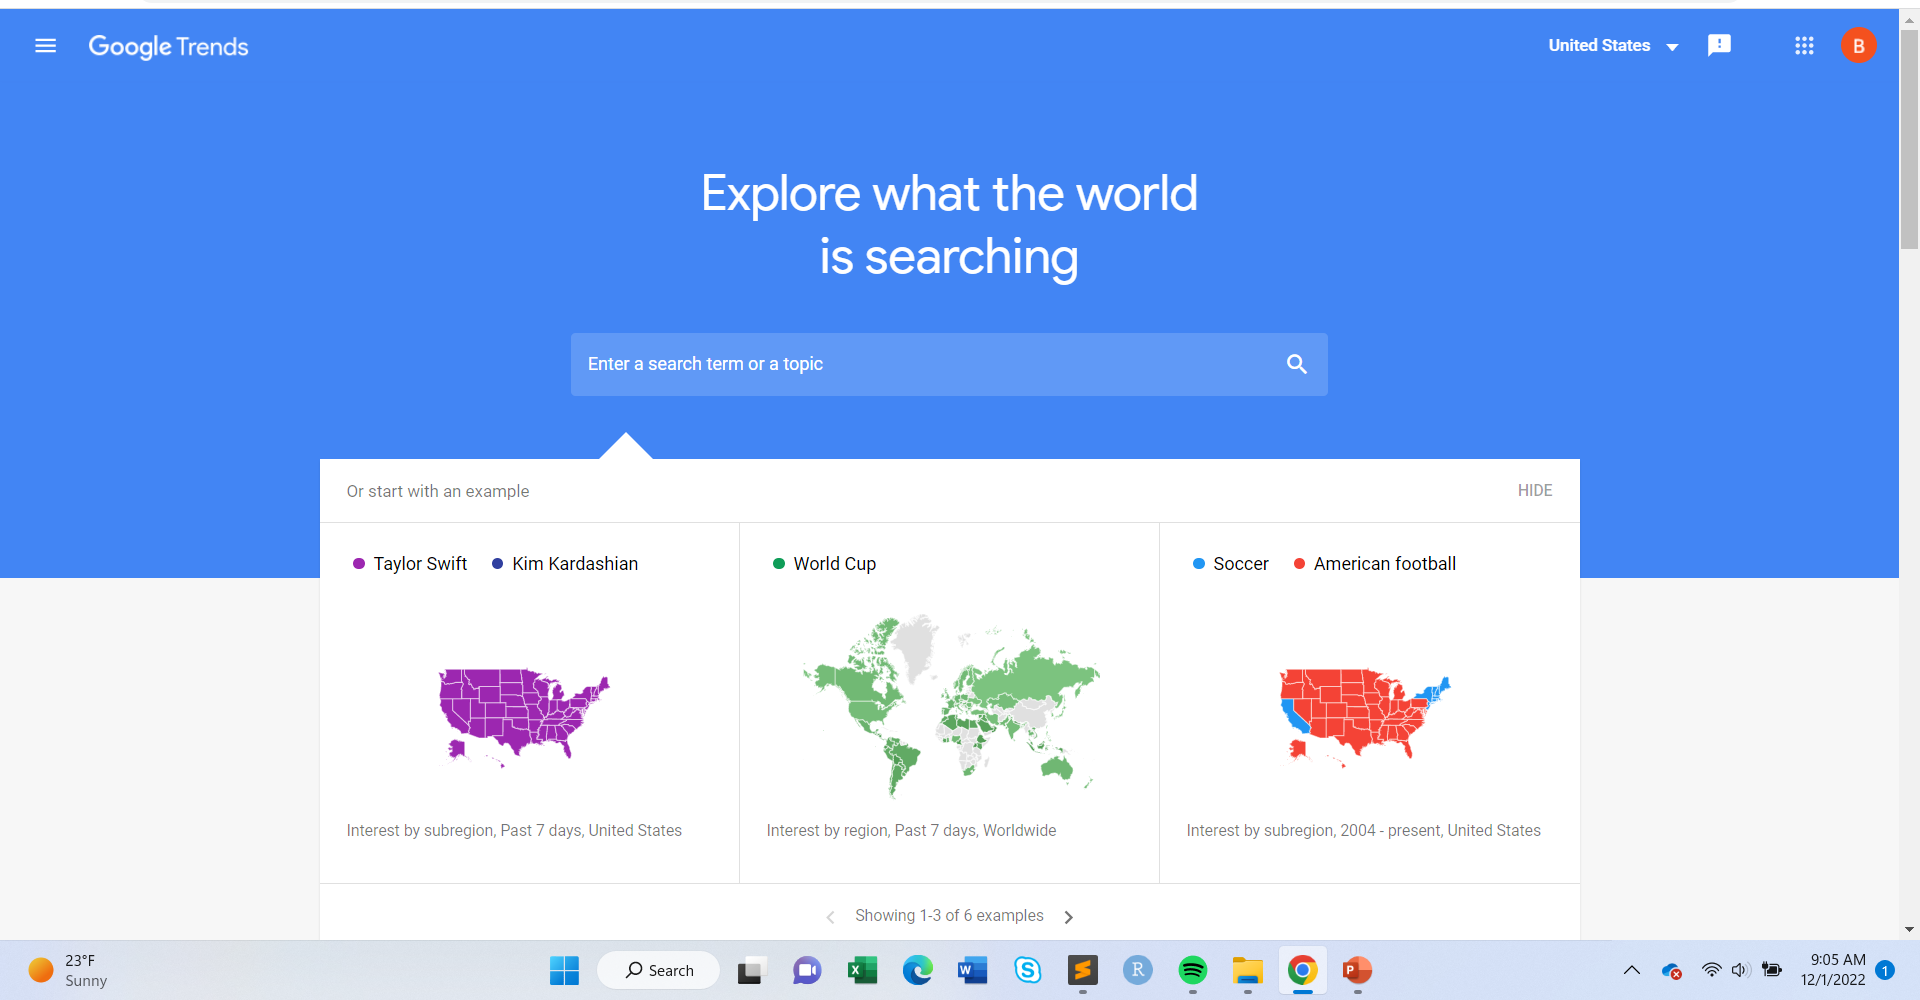
\includegraphics[height=5.6cm, trim=0.0cm 0.0cm 0.0cm 0.0cm width=5.6cm]{Images/Google_Trends_1_120122.png}
  \caption{Figure {\color{franklinblue} 1}: Google Trends Landing Page on 12/1/22}
\end{figure}
\end{frame}

\begin{frame}[t]{GT 12/1/22 Time Series Plot for ``World Cup''}
\begin{figure}[htbp]
  \captionsetup{justification=centering}
  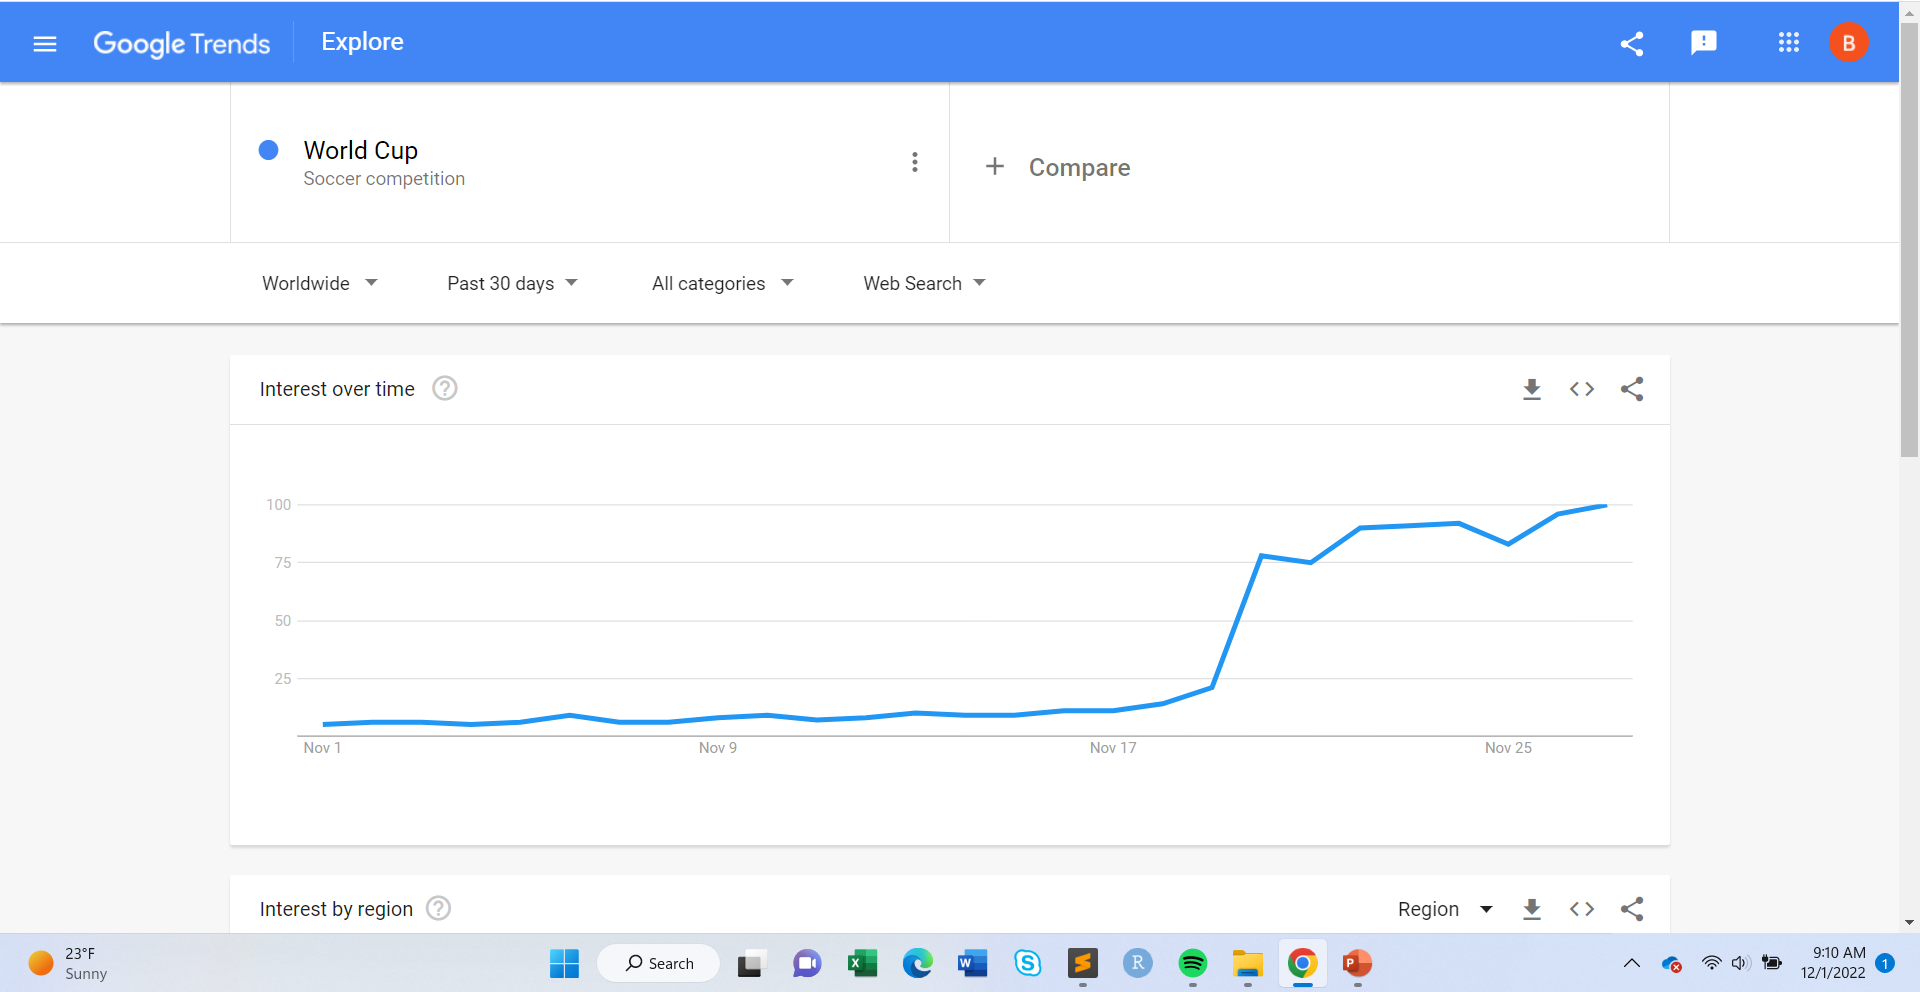
\includegraphics[height=5.6cm, trim=0.0cm 0.0cm 0.0cm 0.0cm width=5.6cm]{Images/Google_Trends_2_120122.png}
  \caption{Figure {\color{franklinblue} 2}: Google Trends 12/1/22 Time Series Plot \\ for Keyword ``World Cup''}
\end{figure}
\end{frame}

\begin{frame}[t]{GT 12/1/22 Country Map for ``World Cup''}
\begin{figure}[htbp]
  \captionsetup{justification=centering}
  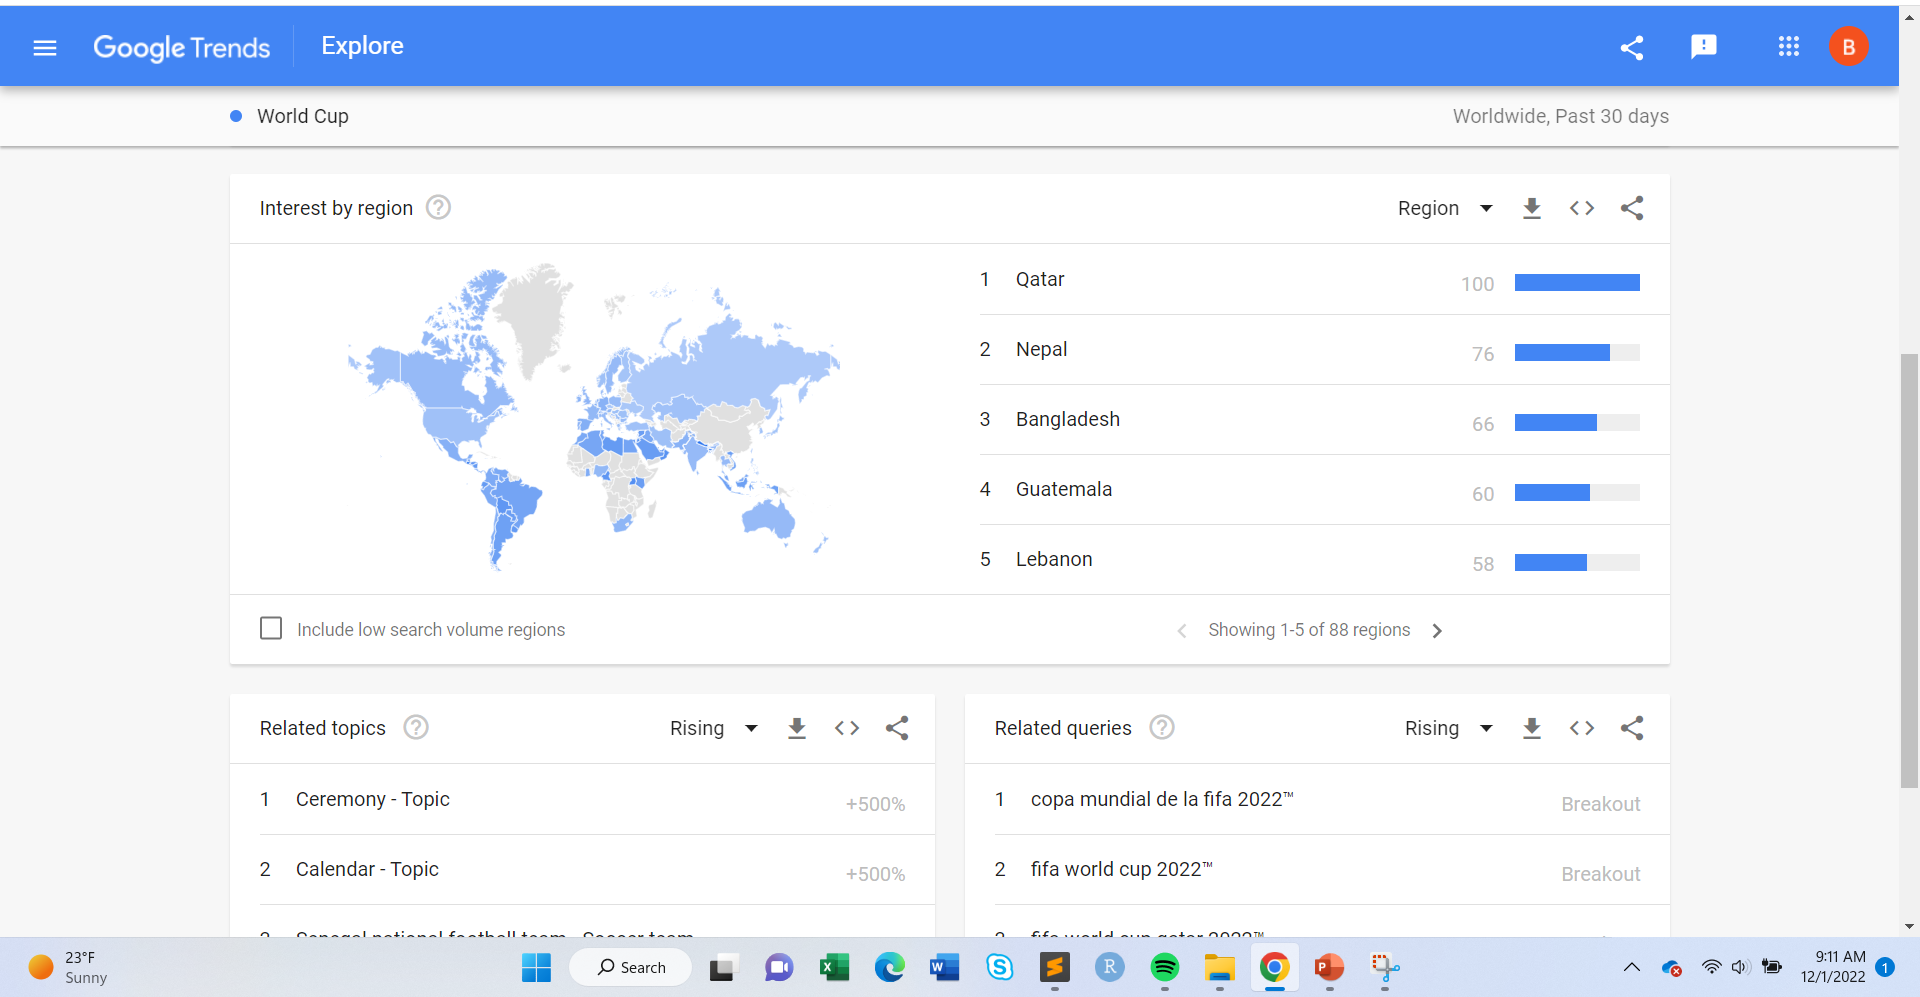
\includegraphics[height=5.6cm, trim=0.0cm 0.0cm 0.0cm 0.0cm width=5.6cm]{Images/Google_Trends_3_120122.png}
  \caption{Figure {\color{franklinblue} 3}: Google Trends 12/1/22 Country Map \\ for Keyword ``World Cup''}
\end{figure}
\end{frame}

\begin{frame}[t]{Is GT a Quality Data Source?}
The main quality dimensions of data at the record level are accuracy, completeness, consistency and validity (\cite{karr2006}). \\
\vspace{1.5ex}
\small
\begin{enumerate}
  \item \empr{Accuracy} pertains to a variable measuring what it is expected to measure. Coverage biases, sampling defects, or non responses may characterize how accurate a source is.
  \item A record is \empr{complete} when it includes values for all attributes.
  \item \empr{Consistency} refers to the situation in which the relationships among the attribute values in the same record are valid. A lack of consistency is, for instance, a starting date after the end date. 
  \item An attribute value is \empr{valid} when it is within a pre-established domain of acceptable values. For example, a person's age can only be a positive number. Ensuring attribute value validity is not enough for ensuring accuracy, although it is a necessary condition.
\end{enumerate}
\end{frame}

\begin{frame}[t]{Caution is Advised When Using GT}
\small
\begin{itemize}
\item GT presents an issue in terms of accuracy, derived from the fact that the reports are generated from a sample of searches made by users (\cite{choi2012}). The sampling methods are not disclosed by Google, so it is not possible to quantify the sampling error.\footnote{For an empirical analysis of the accuracy of GT data, see \cite{cebrian2022}.} 
\item GT includes data for all the observations, although it does not mean that a value is provided for each time period, say, due to small search popularity. Since `0' values precisely represent low popularity, the lack of completeness is not a major issue.  
\item Consistency is not an issue with GT since date and SVI are always returned.
\item Though there are instances where SVI is reported as a negative value, in general the GT data is valid.
\end{itemize}
\end{frame}

\begin{frame}[t]{Online Content Count Tool}
An \empr{online content count tool} calculates frequencies of word or phrases embedded within a media provider's website.
\begin{figure}[htbp]
  \captionsetup{justification=centering}
  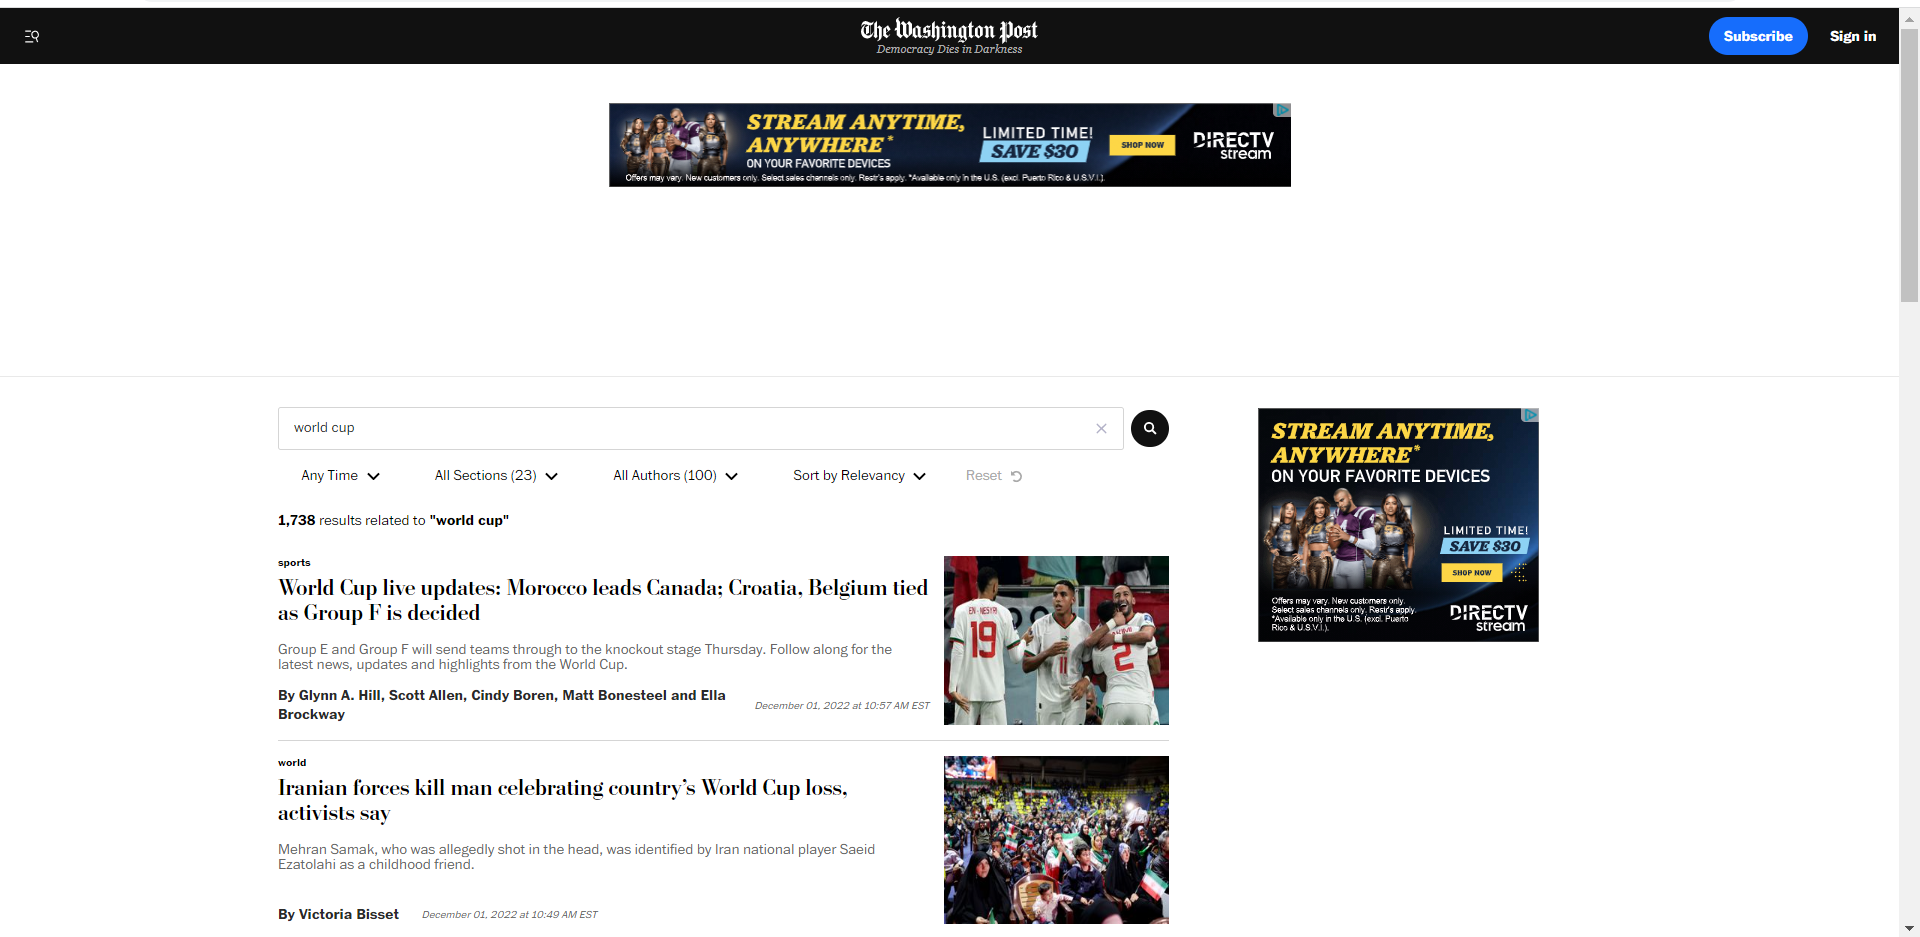
\includegraphics[height=5.0cm, trim=0.0cm 0.0cm 0.0cm 0.0cm width=5.0cm]{Images/Wash_Post_Content_Tool_120122.png}
  \caption{Figure {\color{franklinblue} 4}: Returned page of Washington Post's Online Content  \\ Count Tool for 12/1/22 and Keyword ``world cup''}
\end{figure}
\end{frame}

\begin{frame}[t]{Commercial Data}
Recall from Module 2 that \empr{third party data}, also called syndicated data, are data includes data purchased from a provider such as, \href{https://www.iriworldwide.com/en-us}{IRI}, \href{https://www.nielsen.com/}{Nielsen}, \href{https://nielseniq.com/global/en/}{NielsenIQ}, \href{https://www.npd.com/}{NPD}, or \href{https://www.spins.com/}{Spins}. \\
\vspace{1.5ex}
The \href{https://cloud.google.com/}{Google Cloud} also has many \href{https://cloud.google.com/datasets}{commercial databases} available for purchase. 
\end{frame}

\begin{frame}[t]{Public Data}
\empr{Public data} are data available without purchase.\footnote{There may limitations on who may have access to the data and how the data may be used.} Sources include:\\
%https://www.chicagobooth.edu/research/kilts/datasets/nielsenIQ-nielsen
\vspace{-0.5ex}
\small
\begin{itemize}
  \item National and local governments.  For example, \href{https://fred.stlouisfed.org/}{FRED} data as maintained by the St. Louis Fed.
  \item Private firm public data, such as \href{https://docs.aws.amazon.com/forecast/latest/dg/weather.html}{Amazon Web Services weather data}.
  \item Google makes available various public datasets via the \href{https://console.cloud.google.com/marketplace/browse?filter=solution-type:dataset&_ga=2.201899609.935088507.1674489775-2008566173.1674489775}{Google Cloud}.
 \end{itemize}
 \normalsize
 \vspace{-0.5ex}
 Academic maintained data, such as Nielsen and NielsenIQ data maintained by the \href{https://www.chicagobooth.edu/research/kilts/research-data}{University of Chicago's Kilt's Center for Marketing}.  This data is for academic research only. \\
\vspace{1.5ex}
\href{https://www.statista.com/}{Statista}  is a good place to begin to identify data sources and availability. 
%\href{https://www.webfx.com/blog/marketing/data-sources/
\end{frame}

\section{Social Listening Tools}

\begin{frame}[t]{Social Listening Tools}
\empr{Social listening tools} are platforms that connect to various social media networks in order to extract consumer data.  \\
\vspace{1.5ex}
Social listening tools connect to Facebook, YouTube, WhatsApp, \ldots and extract data from them. \\
\vspace{1.5ex}
Some social listening tools can handle several platforms while others focus solely on one platform. \\
\vspace{1.5ex}
Social listening tools have become increasingly more important as firms are looking for more and more information to help them make better marketing decisions
%https://blog.hootsuite.com/simon-kemp-social-media/
\end{frame}

\begin{frame}[t]{Ranking of Social Media by Global Active Users}
\begin{figure}[htbp]
  \captionsetup{justification=centering}
  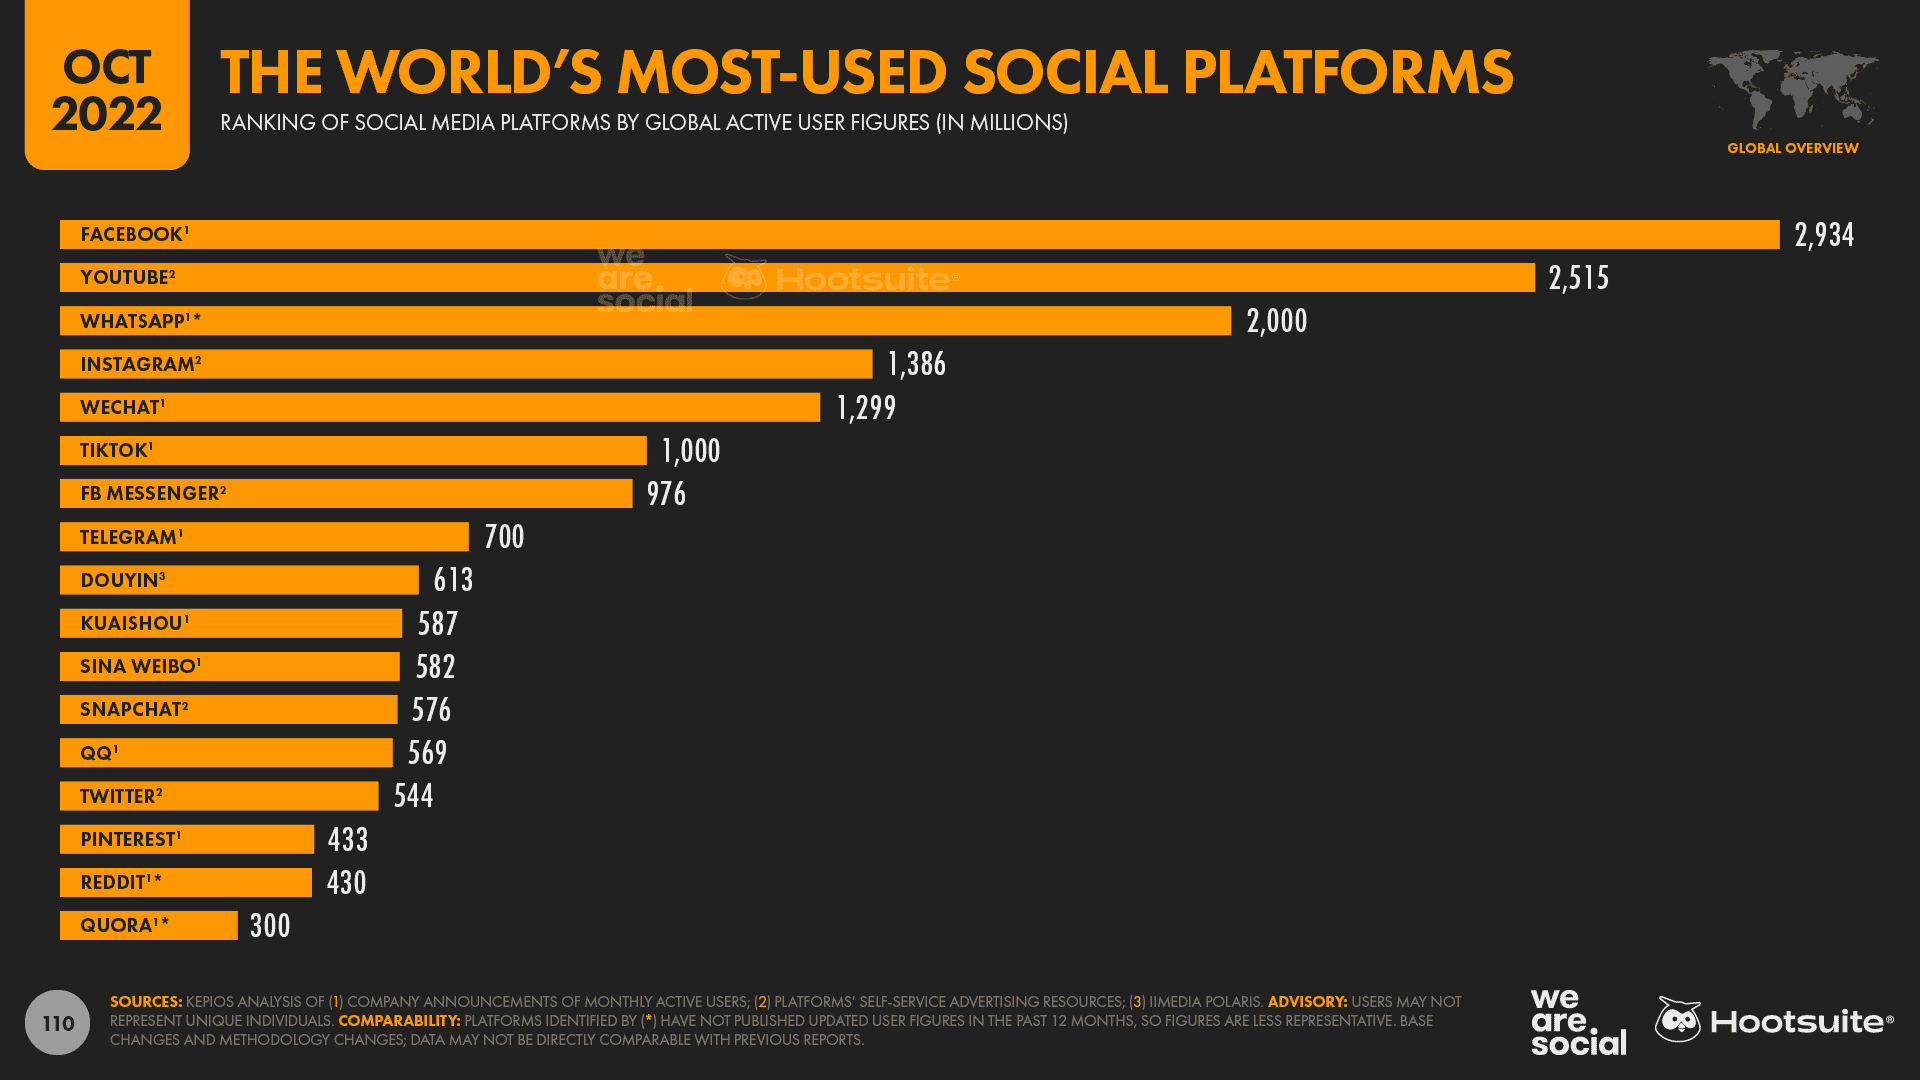
\includegraphics[height=5.9cm, trim=0.0cm 0.0cm 0.0cm 0.0cm width=5.9cm]{Images/Hootsuite_SocialMedia_1022_1.png}
  \caption{Figure {\color{franklinblue} 5}: Ranking of Social Media Platforms by  \\ Global Active Users in Millions}
\end{figure}
\end{frame}

\begin{frame}[t]{Average Time Per Month For Android App Users}
\begin{figure}[htbp]
  \captionsetup{justification=centering}
  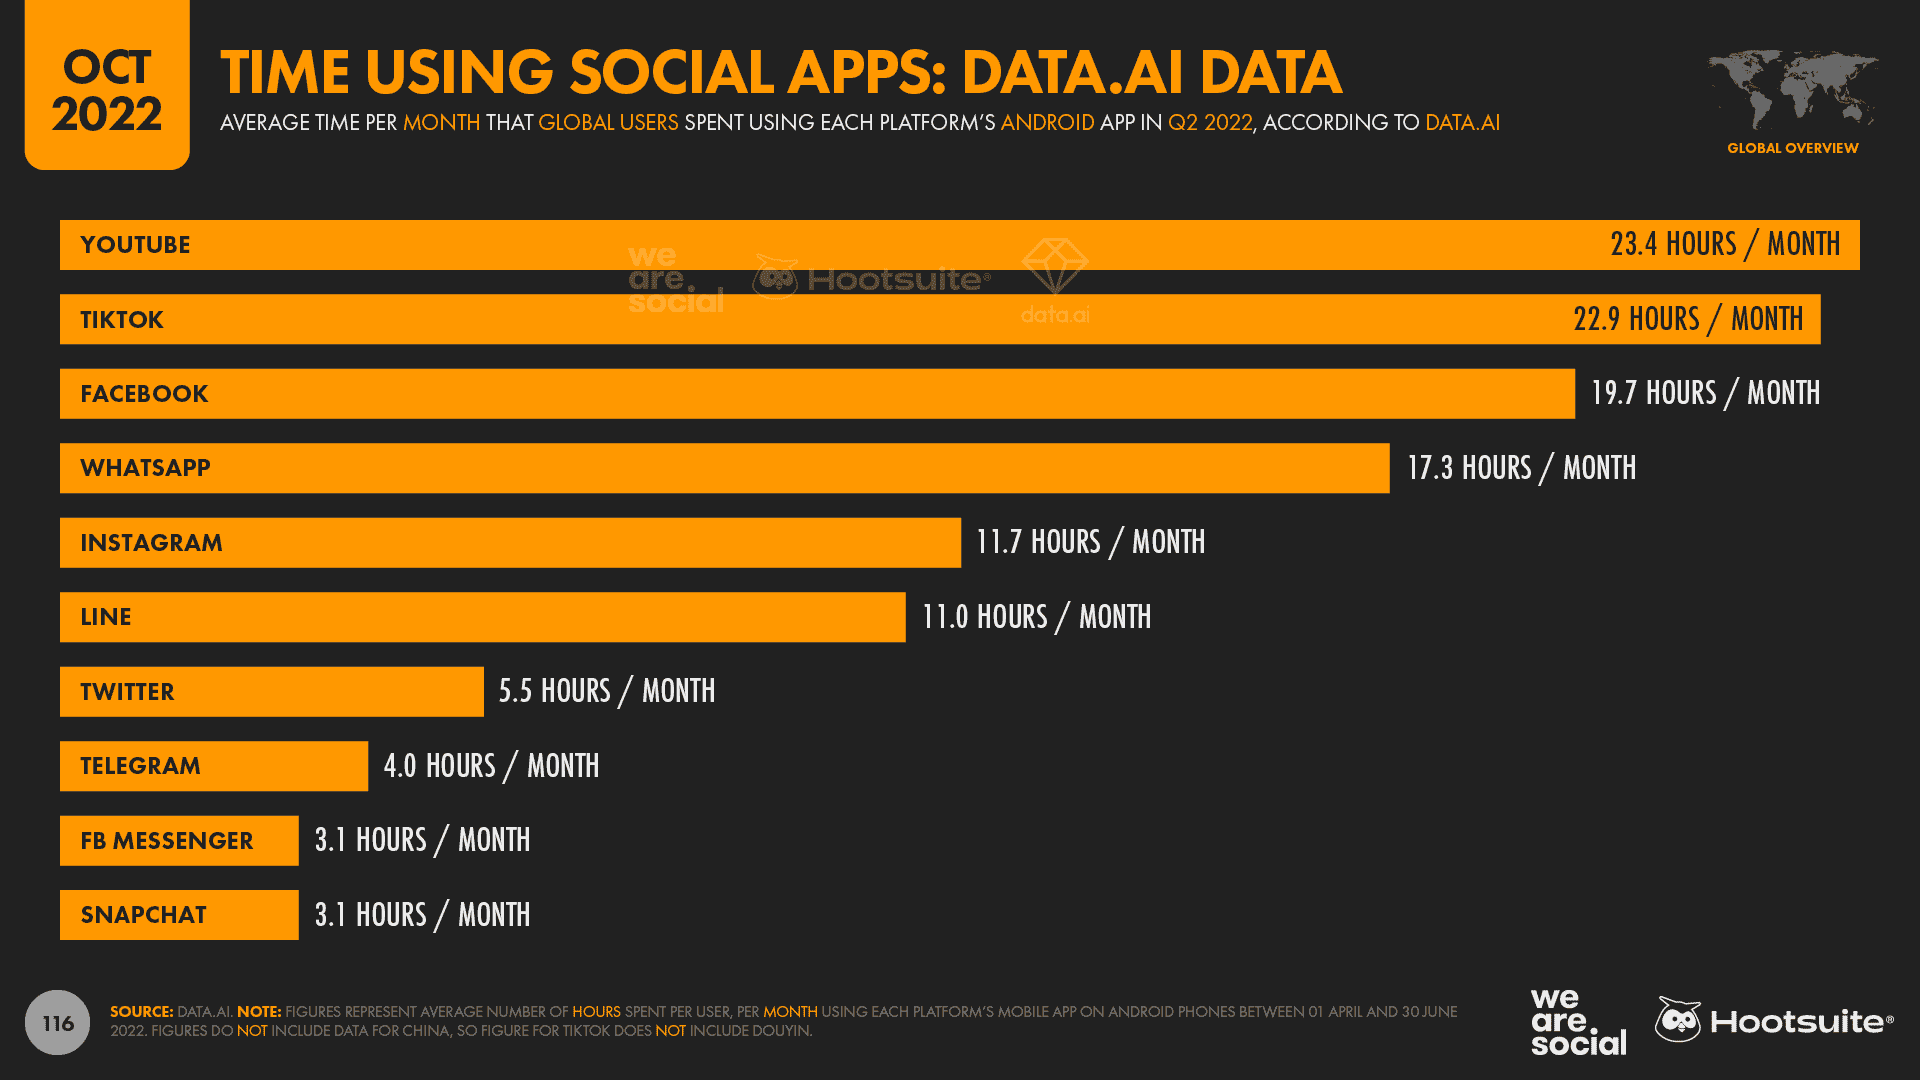
\includegraphics[height=5.9cm, trim=0.0cm 0.0cm 0.0cm 0.0cm width=5.9cm]{Images/Hootsuite_SocialMedia_1022_2.png}
  \caption{Figure {\color{franklinblue} 6}: Average Time Per Month That Global Users Spent \\ Using Each Platforms Android App in Q2 2022}
\end{figure}
\end{frame}

\begin{frame}[t]{\% of Social Media Platform Users on Other Platforms}
\begin{figure}[htbp]
  \captionsetup{justification=centering}
  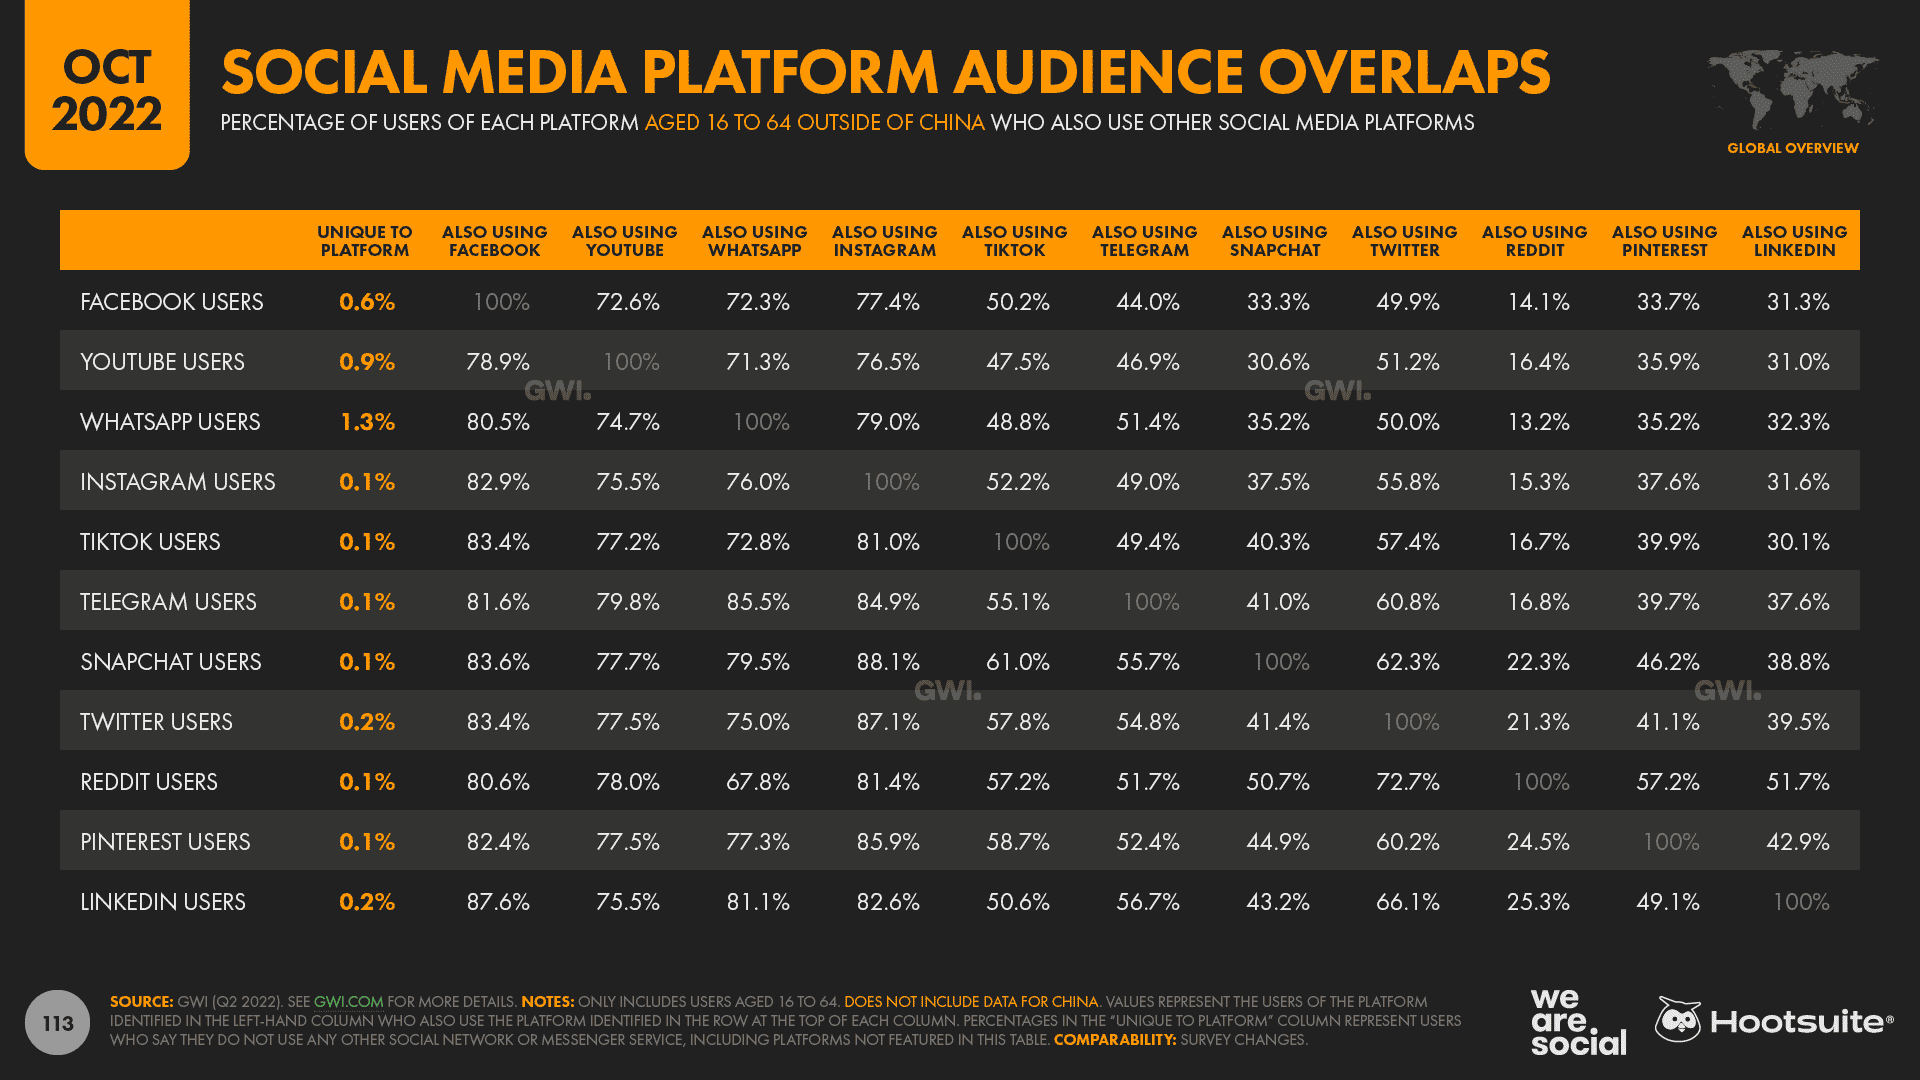
\includegraphics[height=5.9cm, trim=0.0cm 0.0cm 0.0cm 0.0cm width=5.9cm]{Images/Hootsuite_SocialMedia_1022_3.png}
  \caption{Figure {\color{franklinblue} 7}: Percentage of Users of Each Platform Aged 16 to 64 \\ Outside of China Who Also Use Other Social Media Platforms}
\end{figure}
\end{frame}

\begin{frame}[t]{Social Listening Tools Purpose}
A \empr{single-attribute social listening tool} focuses on one social media characteristic such as text or image content. For example, tools that focus only on reading blog posts would be single-attribute. \\
\vspace{1.5ex}
\empr{Multi-platform social listening tools} allow marketing analytics professionals to see data across many social media platforms, say across Snapchat, Pinterest, and Twitter. \\
\vspace{1.5ex}
A \empr{native social listening tool} is a social media platform specific application that provides detailed analytics about who is interacting with the organization's platform content. The textbook mentions that \href{https://www.hootsuite.com/}{Hootsuite}, \href{https://partners.twitter.com/en/partners/union-metrics}{Union Metrics (formerly TweetReach)}, and \href{https://tweeplesearch.com}{Tweeple Search} are good examples of social listening tools.\footnote{The textbook does not mention that Union Metrics was acquired by Trendkite, which was subsequently acquired by \href{https://www.cision.com/}{Cision}.}
\end{frame}

\begin{frame}[t]{Hootsuite Marketing Collateral and Information}
\begin{figure}[htbp]
  \captionsetup{justification=centering}
  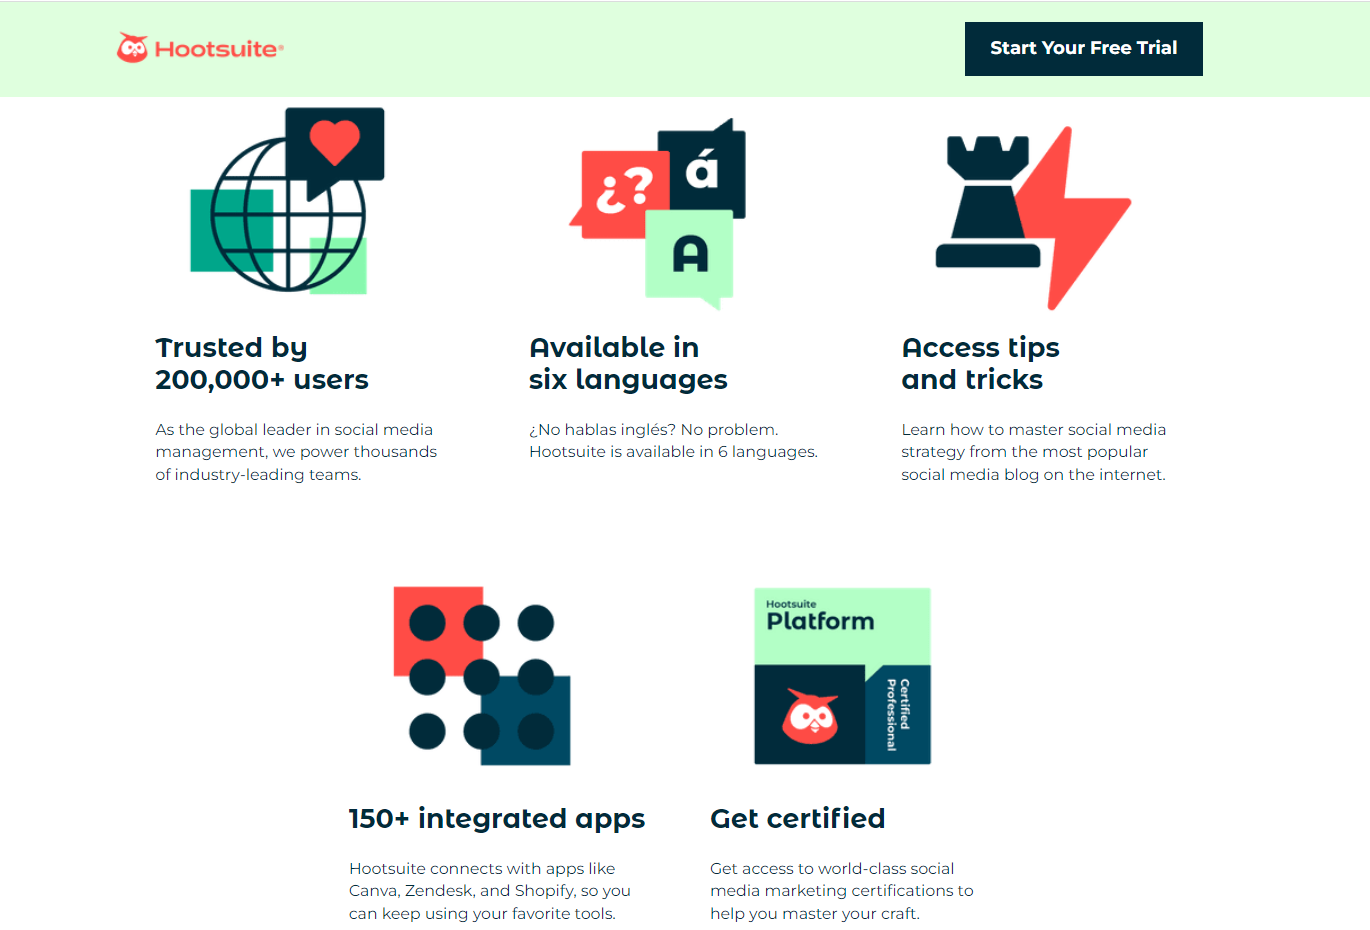
\includegraphics[height=6.6cm, trim=0.0cm 0.0cm 0.0cm 0.0cm width=6.6cm]{Images/Hootsuite_SocialMedia_1022_4.png}
  \caption{Figure {\color{franklinblue} 8}: Hootsuite Marketing Collateral and Information}
\end{figure}
\end{frame}

\begin{frame}[t]{Audience Insight Marketing Collateral and Information}
\begin{figure}[htbp]
  \captionsetup{justification=centering}
  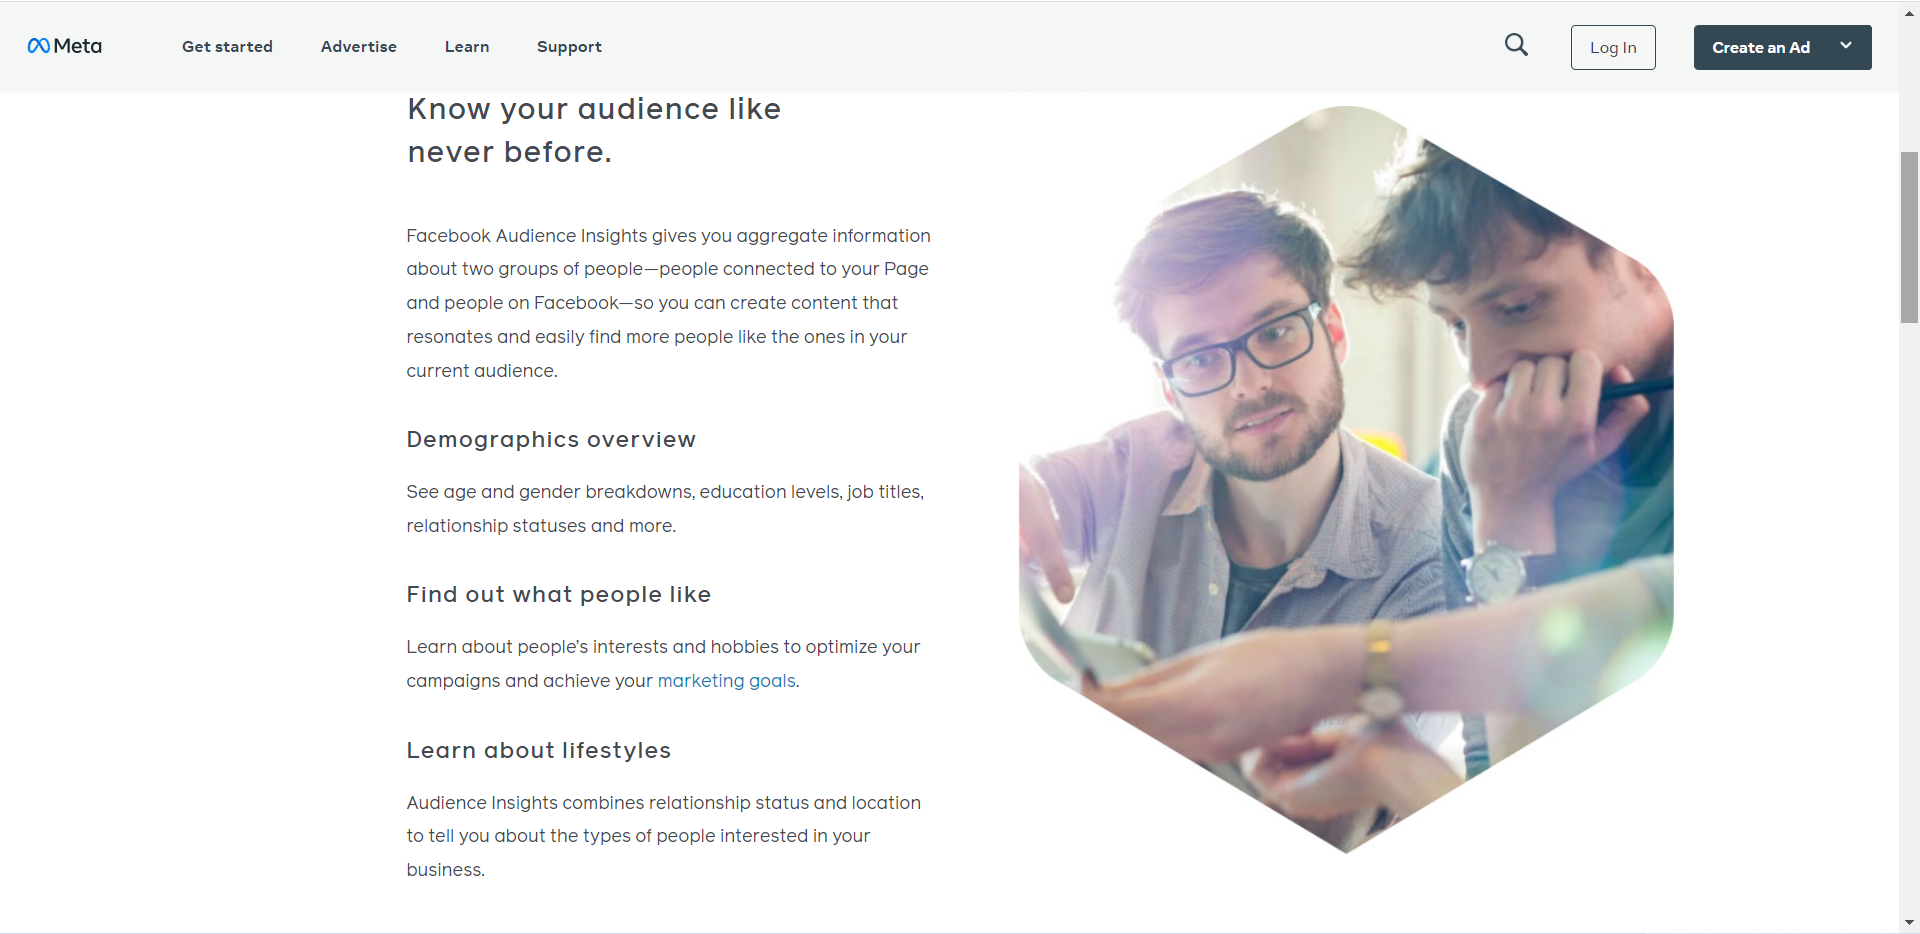
\includegraphics[height=5.2cm, trim=0.0cm 0.0cm 0.0cm 0.0cm width=5.2cm]{Images/Facebook_Audience_Insights_120122.png}
  \caption{Figure {\color{franklinblue} 9}: Facebook Audience Insight Marketing \\ Collateral and Information}
\end{figure}
\end{frame}

\section{Web Analytics}

\begin{frame}[t]{Defining Web Analytics}
\href{https://www.gartner.com/en/information-technology/glossary/web-analytics}{Gartner} defines \empr{web analytics} as specialized analytic applications used to understand and improve online channel user experience, visitor acquisition and actions, and to optimize digital marketing and advertising campaigns. \\
\vspace{1.5ex}
\begin{itemize}
\item Commercial products offer reporting, segmentation, analytical and performance management, historical storage and integration with other data sources and processes. 
\item The tools are used by marketing professionals, advertisers, content developers and the website's operations team, and increasingly provide input to automated tools that target improved customer experience. 
\end{itemize}
\end{frame}

\begin{frame}[t]{Distinguishing Google Analytics and Google Ads}
%https://www.leadfeeder.com/blog/google-analytics-alternatives/
While Google Analytics (GA) has a large share of the web analytics market, competitors include \href{https://www.leadfeeder.com/}{Leadfeeder}, \href{https://piwik.pro/}{Piwik Pro Analytics Suite}, \href{https://www.smartlook.com/}{Smartlook}, and \href{https://www.woopra.com/}{Woopra}.
\begin{itemize}
\item Challenges with GA include the non-negligible effort required to ensure the tool is GDPR compliant, and it is not the simplest tool to learn and use.  
\item To overcome these challenges, Google offers many \href{https://skillshop.exceedlms.com/student/catalog/browse}{courses} on how to set-up and use the service.
\end{itemize}
Google Analytics is \underline{not} Google Ads.  
\begin{enumerate}
  \item \href{https://marketingplatform.google.com/about/analytics/}{Google Analytics} is a web analytics service offered by Google that tracks and reports website traffic, currently as a tool inside the \href{https://support.google.com/marketingplatform/answer/9013946?hl=en}{Google Marketing Platform}. 
\end{enumerate}
\end{frame}

\begin{frame}[t]{Specifying Google Ads}
\begin{enumerate}
  \setcounter{enumi}{1}
    \item \href{https://ads.google.com/home/faq/}{Google Ads}, previously Google AdWords and Google AdWords Express, is an online advertising solution that businesses use to promote their products and services on Google Search, YouTube, and other sites across the web.
    \begin{itemize}
      \item Google Ads also allows advertisers to choose specific goals for their ads, like driving phone calls or website visits. 
      \item With a Google Ads account, advertisers can customize their budgets and targeting, and start or stop their ads at any time. Google ads typically appear on two networks. 
      \begin{itemize}
         \item \href{https://support.google.com/google-ads/answer/1722047}{Google Search Network}, which includes Google search result pages, other Google sites like Maps and Shopping, and partnering search sites. 
         \item \href{https://support.google.com/google-ads/answer/2404190?hl=en}{Google Display Network}, which includes Google sites like YouTube, Blogger, and thousands of partnering websites.
      \end{itemize}
    \end{itemize}
\end{enumerate}
\end{frame}

\begin{frame}[t]{Google Analytics 4 is the Next Version of GA}
% The remainder of the content below is mostly sourced from the GA4 tutorial as of 9/19/23 - https://skillshop.exceedlms.com/student/catalog/list?category_ids=6431-google-analytics-4 
On July 1, 2023, the pre-existing and standard GA default property \empr{Universal Analytics} would no longer process data.\footnote{Via a \href{https://support.google.com/analytics/answer/11583528?hl=en}{one-time processing extension}, one will be able to see Universal Analytics reports until July 1, 2024.  Some refer to Universal Analytics as ``Analytics Classic''.} \\
\vspace{1.5ex}
Data will only flow into \href{https://support.google.com/analytics/answer/10089681?hl=en}{\empr{Google Analytics 4}} (GA4), the next version of GA (i.e., replacement of Universal Analytics). \\
\vspace{1.5ex}
This \href{https://support.google.com/analytics/answer/9304153?hl=en}{page} lists the steps required to use GA4 for an organization's website or app, where one step is pasting a Google tag (i.e., a JavaScript snippet for a website) immediately after the {\color{treegreen} \texttt{<head>}} on each page of the organization's website or using a \href{https://opensource.google/projects/firebasesdk}{Firebase software development kit (SDK)} for an app. \\
\end{frame}

\begin{frame}[t]{You Are in the Midst of GA4 Tutorials}
\begin{figure}[htbp]
  \captionsetup{justification=centering}
  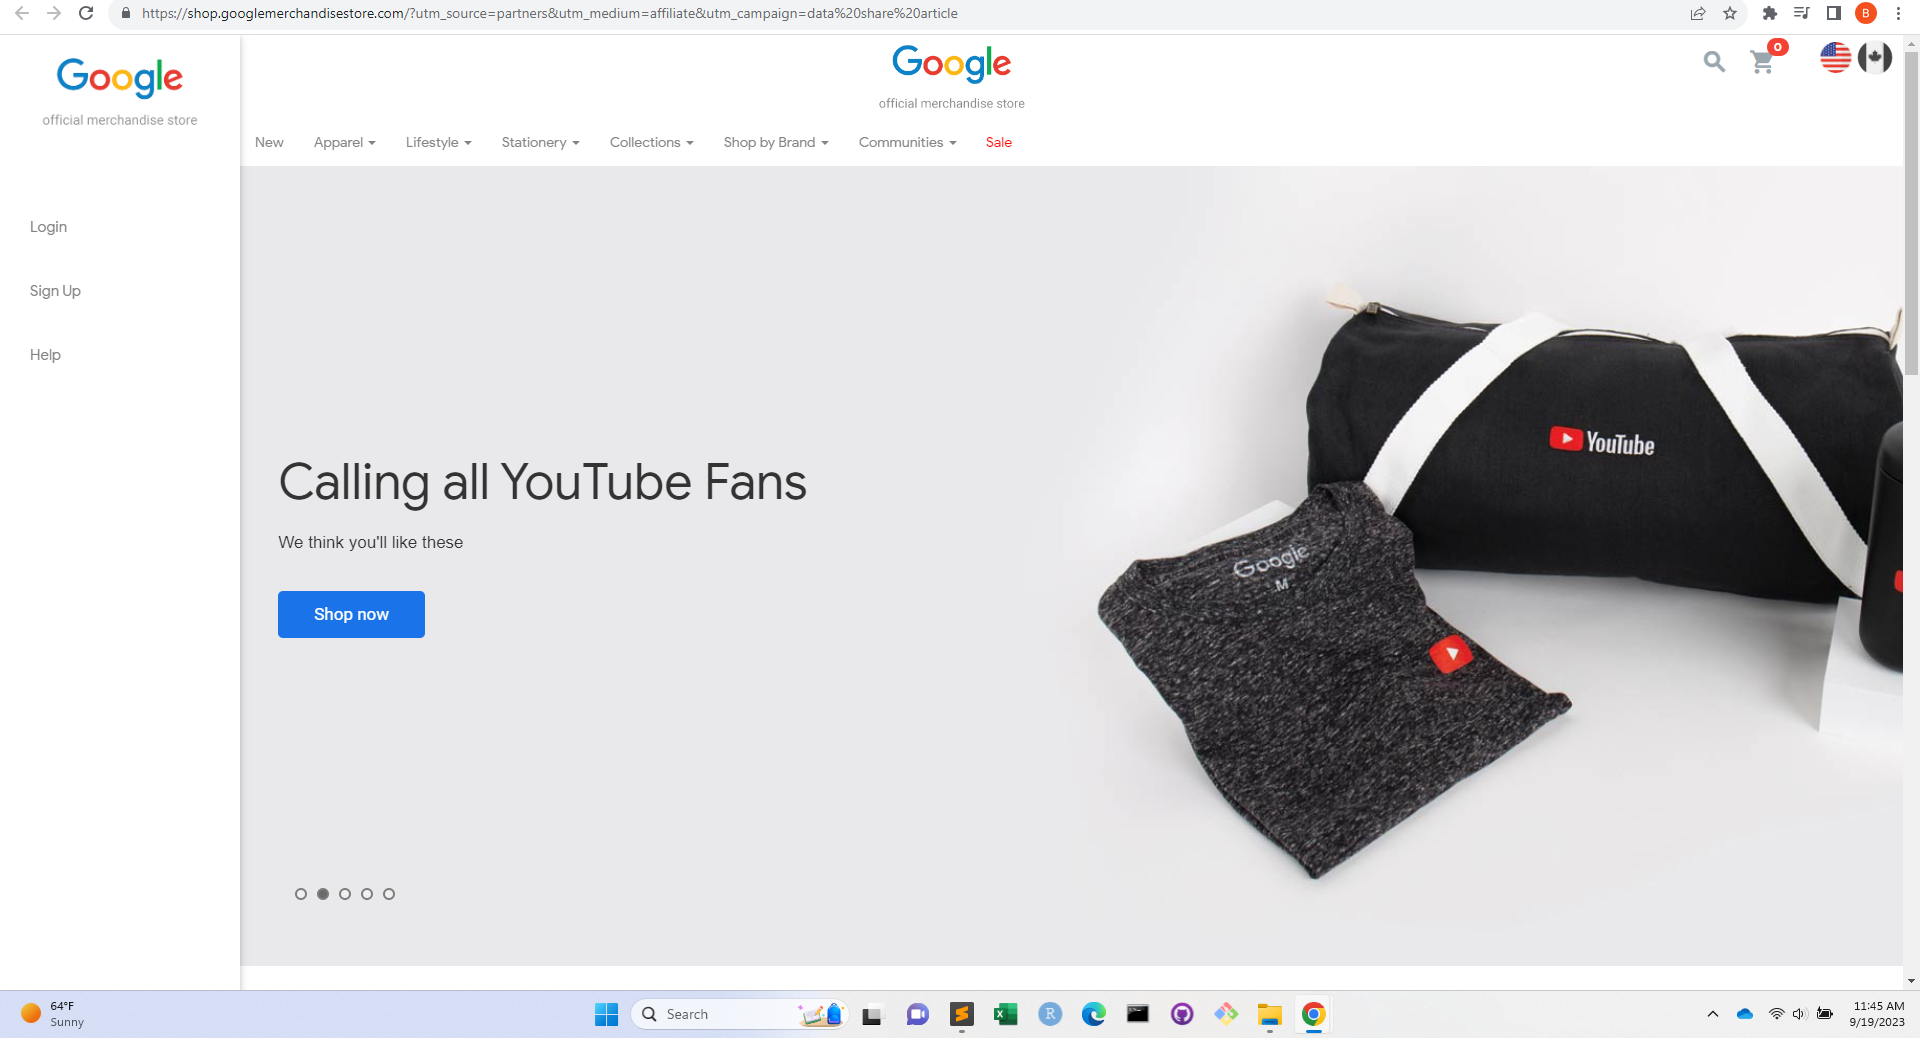
\includegraphics[height=5.6cm, trim=1.5cm 0.0cm 2.0cm 0.0cm width=5.6cm]{Images/GA4_1_091923.png}
  \caption{Figure {\color{franklinblue} 10}: Google Merchandise Store}
\end{figure}
\vspace{-2.0ex}
The Google-provided GA4 demo uses data from either the \href{https://shop.googlemerchandisestore.com/}{Google Merchandise Store} or the app game \href{https://flood-it.app/}{Flood-It!}
\end{frame}

\begin{frame}[t]{Flood-It!}
\begin{figure}[htbp]
  \captionsetup{justification=centering}
  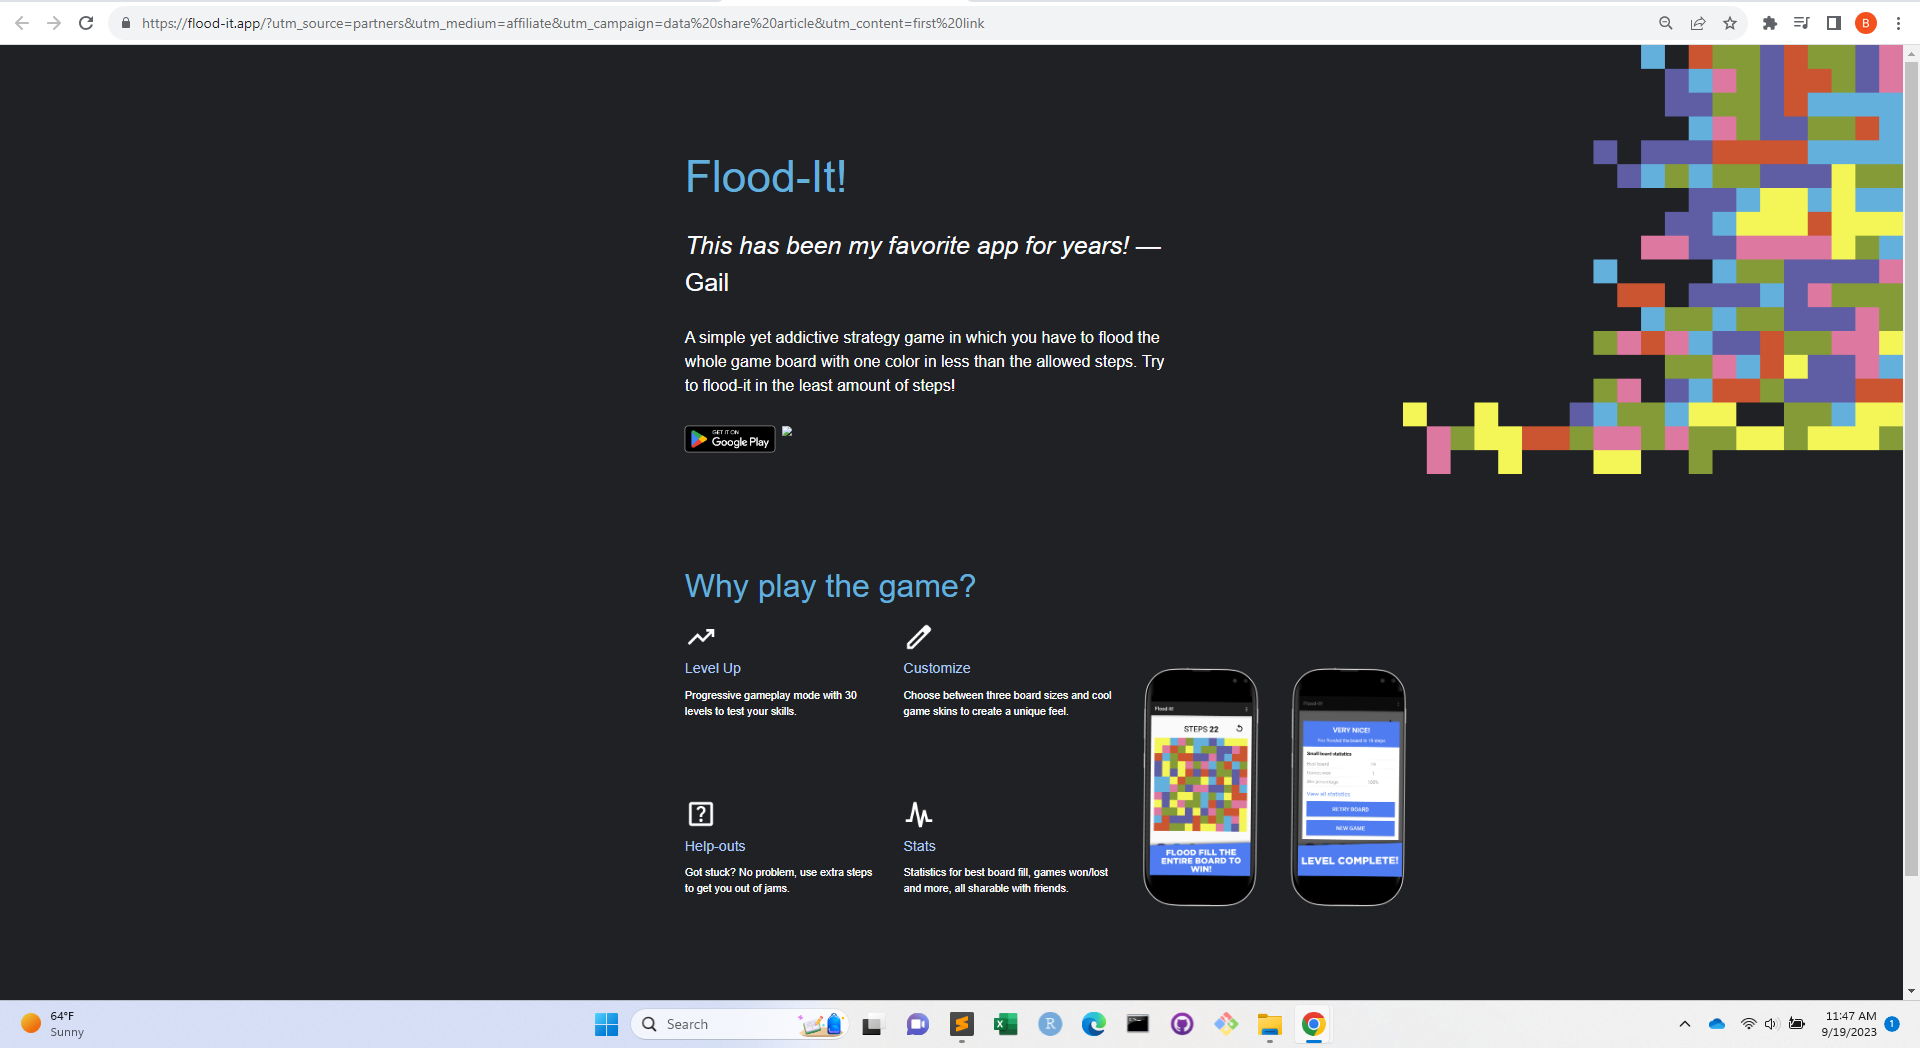
\includegraphics[height=5.6cm, trim=1.5cm 0.0cm 2.0cm 0.0cm width=5.6cm]{Images/GA4_2_091923.png}
  \caption{Figure {\color{franklinblue} 11}: Flood-It!}
\end{figure}
\end{frame}

\begin{frame}[t]{Defining Account, Property and Data Stream}
%https://support.google.com/analytics/answer/1102154?hl=en  
The GA4 \texttt{Admin} pages allows one configure account, properties and data streams.\\
\vspace{1.5ex}
\begin{itemize}
\item An \textit{account} is the access point for GA4. 
\item A \textit{property} is a website, mobile application, or device (e.g., a kiosk or point-of-sale device).  A property lives within an account.\footnote{An account can include multiple properties and property types, but a property can belong to only one GA4 account.} Properties are the containers for GA4 end-user reports based on the data collected from apps and sites. It is the level at which GA4 processes data and where GA4 can connect with other Google products, like Google Ads.
\item A \textit{data stream} lives within a property and is the source of data from the app or website. A property can have one or many data streams.
\end{itemize}
\end{frame}

\begin{frame}[t]{GA4 \texttt{Admin}}
The remainder of the screenshots in this section are for the Google-provided properties ``GA4 - Google Merch Shop'' or ``GA4 - Flood-It!''. 
\begin{figure}[htbp]
  \captionsetup{justification=centering}
  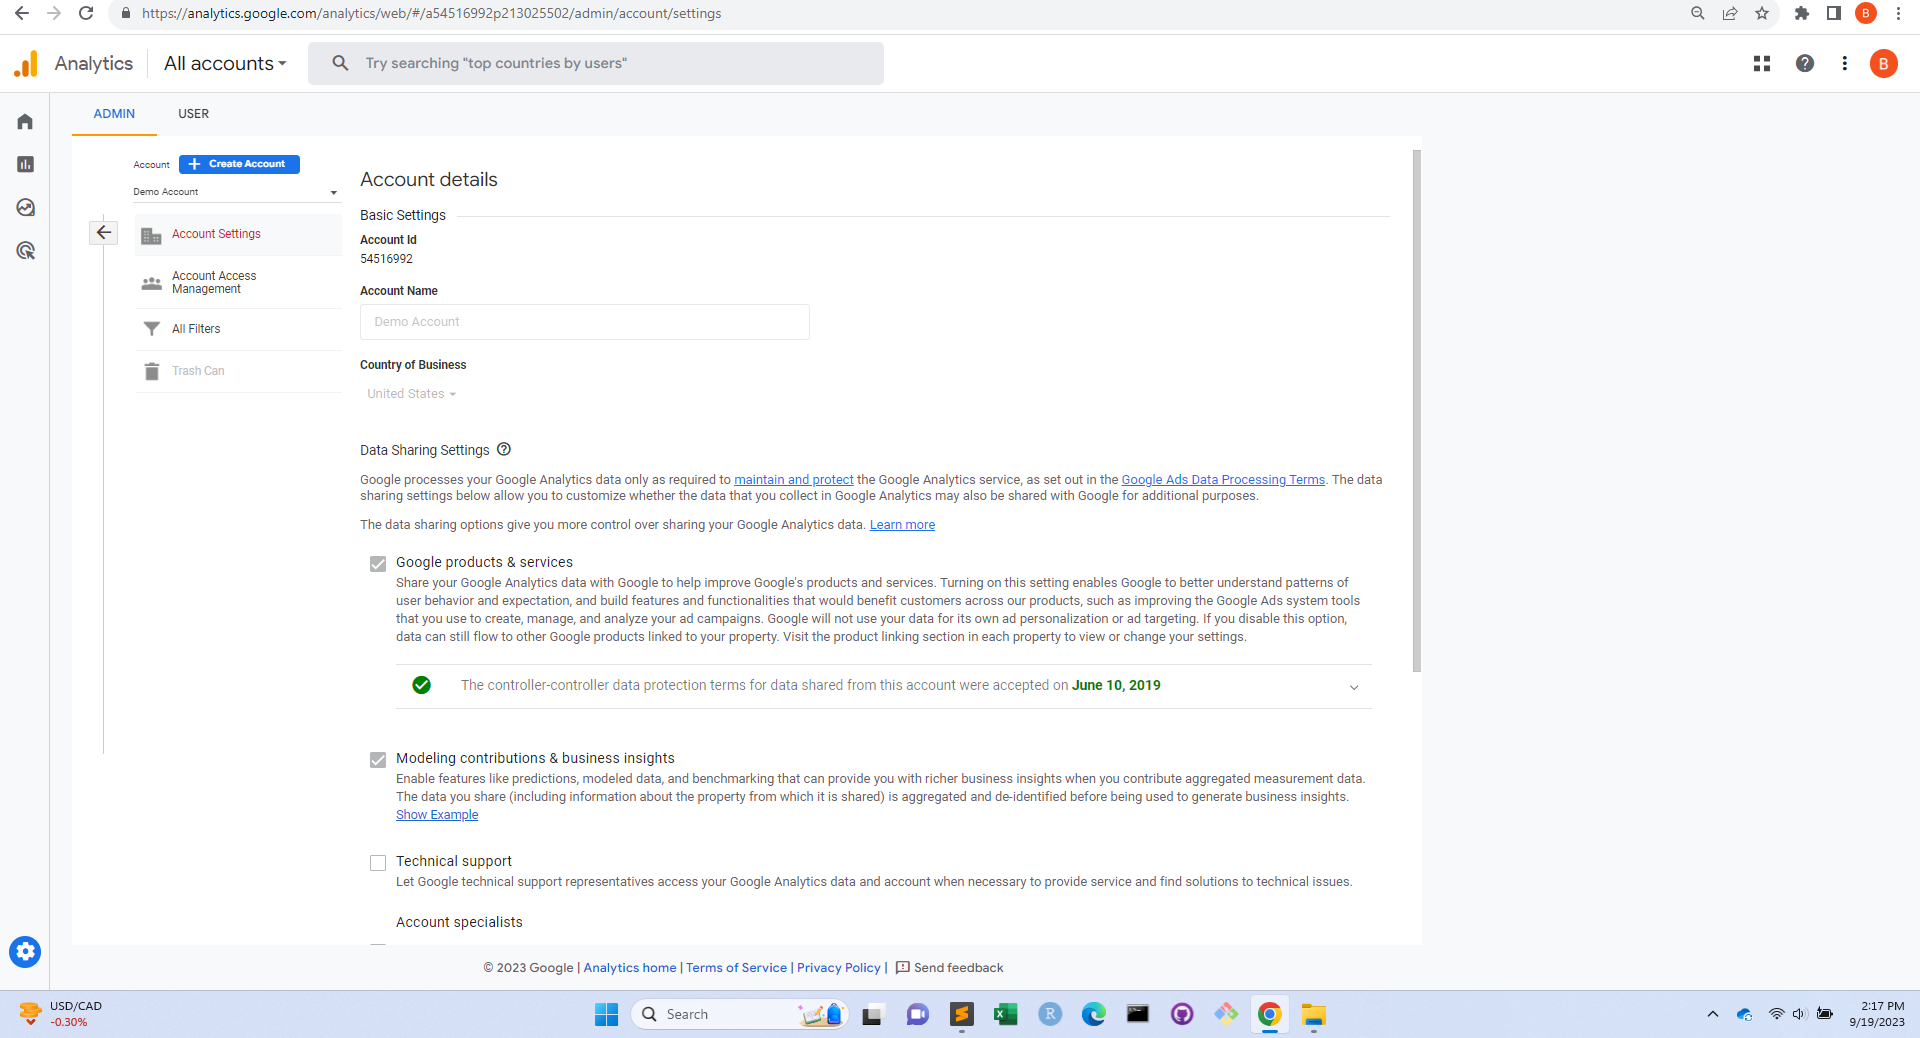
\includegraphics[height=5.3cm, trim=1.5cm 0.0cm 2.0cm 0.0cm width=5.6cm]{Images/GA4_5_091923_Admin.png}
  \caption{Figure {\color{franklinblue} 12}: GA4 \texttt{Admin}}
\end{figure}
\end{frame}

\begin{frame}[t]{GA4 \texttt{Admin} Configuration Options}
\begin{figure}[htbp]
  \captionsetup{justification=centering}
  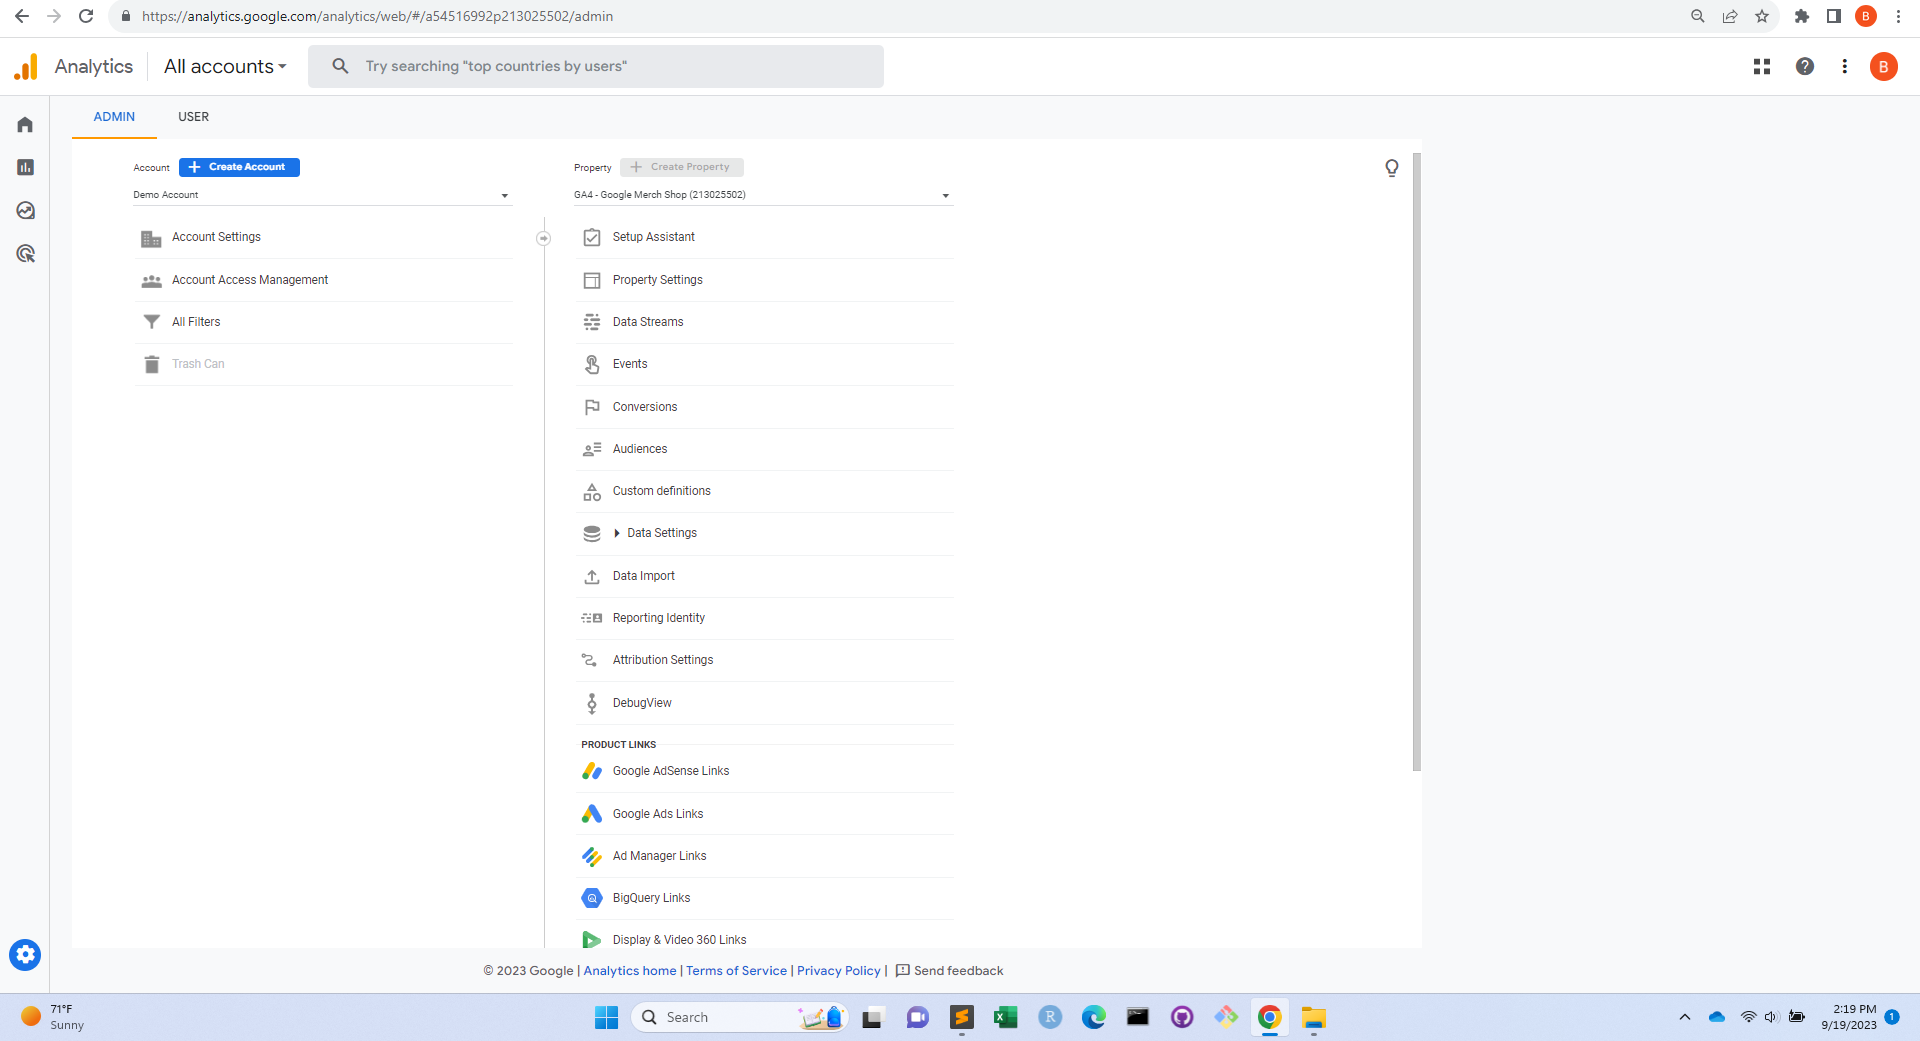
\includegraphics[height=5.6cm, trim=1.5cm 0.0cm 2.0cm 0.0cm width=5.6cm]{Images/GA4_4_091923_Admin.png}
  \caption{Figure {\color{franklinblue} 13}: GA4 \texttt{Admin} Configuration Options}
\end{figure}
\vspace{-2.0ex}
\texttt{Admin} has many configurable options, where the \texttt{Setup Assistant} may be used.  
\end{frame}

\begin{frame}[t]{Events, Parameters, User Properties and  Conversions}
\textit{Events} are user interactions with a website or app that can be measured, like a video view. \\
\vspace{1.5ex}
\textit{Event parameters} are additional pieces of information sent with events that can further specify an action the user took or add further context to the event, like the name of the video or how long the user watched it. \\
\vspace{1.5ex}
\textit{User properties} are attributes about who is using the organization's app or website that can help end-users better understand segments of the organization's user base, like geographic location or device used. \\
\vspace{1.5ex}
A \textit{conversion} is an event that one considers important to the organization, such as a purchase or a download. One may want to share conversions with marketing platforms, like Google Ads.
\end{frame}

\begin{frame}[t]{Dimensions, Metric and Their Values}
\textit{Dimensions} answer the question, ``Who, what, or where?'' While \textit{metrics} answer the question, ``How many?'' For example, dimensions answer the question, ``What device is most commonly used?'' While metrics answer questions like, ``How many users visited the site yesterday?'' \\
\small
\begin{itemize}
\item A \textit{dimension} is a text-based label that represents the data.
\item \textit {Dimension values} are the text values for the dimensions that have been selected. 
\item A \textit{metric} is a numeric value that represents the data.
\item \textit{Metric values} are the the numeric values that are being calculated for the dimension values selected.
\end{itemize}
\end{frame}

\begin{frame}[t]{Managing Events}
Recall GA4 collects and stores user interactions with the website or app as events. Events provide insight into what is happening on the website or app, such as: \\
\small
\begin{itemize}
  \item Clicks and page views on the website.
  \item Installs and opens on the app.
  \item User engagement and conversions on either platform.
\end{itemize}
\normalsize 
Also recall event parameters give additional information with each event.  For example, for a collected page view event, GA4 includes the page's URL as an event parameter value. \\
\vspace{1.5ex}
\underline{Automatically collected} events are triggered by basic interactions with the app and/or site (as indicated under the event name in a GA4 table). As long as one uses the GA4 Firebase SDK or gtag.js additional code to collect these events is unneeded.
\end{frame}

\begin{frame}[t]{GA4 \texttt{Admin} Event Definitions}
\begin{figure}[htbp]
  \captionsetup{justification=centering}
  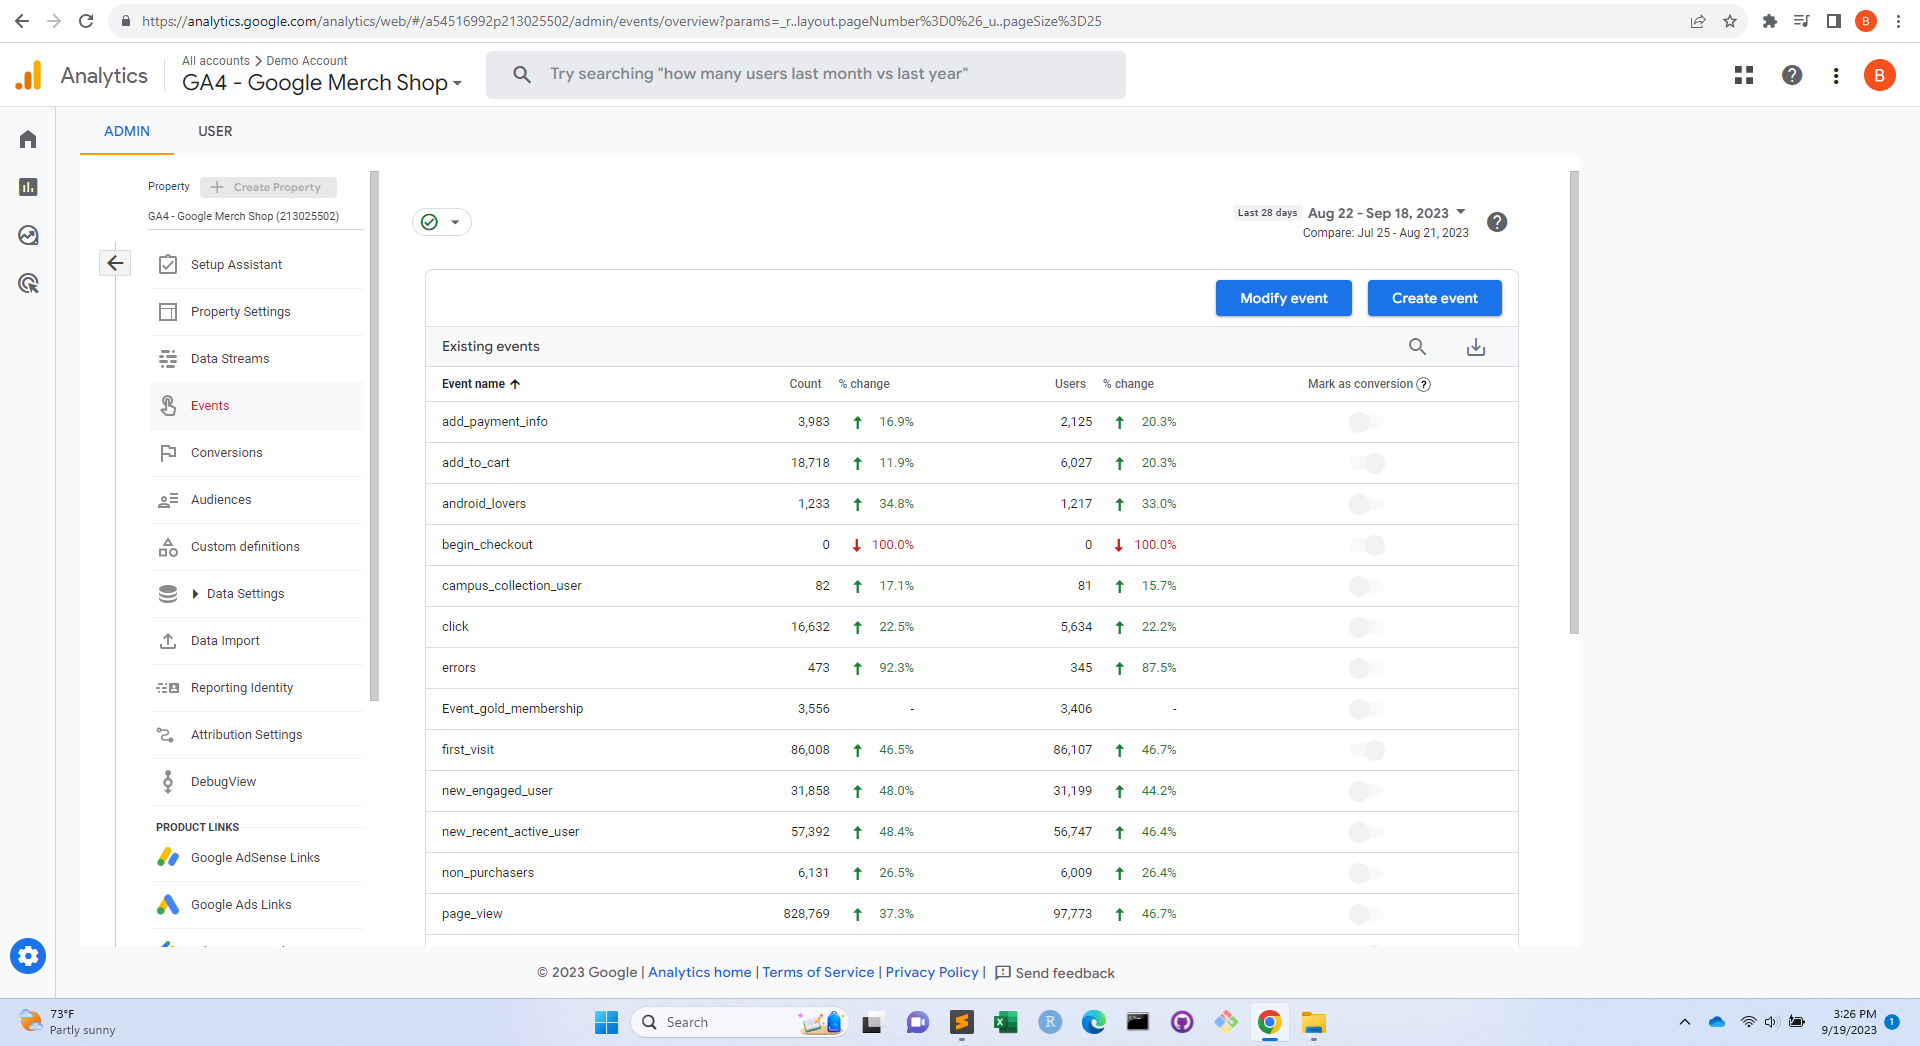
\includegraphics[height=5.6cm, trim=1.5cm 0.0cm 2.0cm 0.0cm width=5.6cm]{Images/G4A_7a_091923_Admin_Events.png}
  \caption{Figure {\color{franklinblue} 14}: GA4 \texttt{Admin} Events}
\end{figure}
\end{frame}

\begin{frame}[t]{Enhanced Measurement}
\small
\textit{Enhanced measurement} lets one measure interactions with a website or app by enabling new events in GA4. No code changes are required.  When enabled for a web data stream the GA4 tag automatically starts sending event information right away. \\
\vspace{1.5ex}
\begin{itemize}
  \item \textit{Recommended events} are those the organization implements, but which have predefined names and parameters already recognized by GA4. Adding these events to the website or mobile app helps one measure additional behavior, as well as generate more useful reports.
  \item  A \textit{custom event} is one whose name and parameters select GA4 end-users define. A custom event lets one collect \underline{specific} business data that GA4 does not otherwise automatically collect.  
\end{itemize}
When one implements new and custom events and their associated parameters on the website or app, one starts sending this new data to GA4. In these cases, one \underline{must} create custom dimensions and metrics that correspond to the data so they will be available in the reports.
\end{frame}

\begin{frame}[t]{GA4 \texttt{Admin} Custom Dimensions}
\begin{figure}[htbp]
  \captionsetup{justification=centering}
  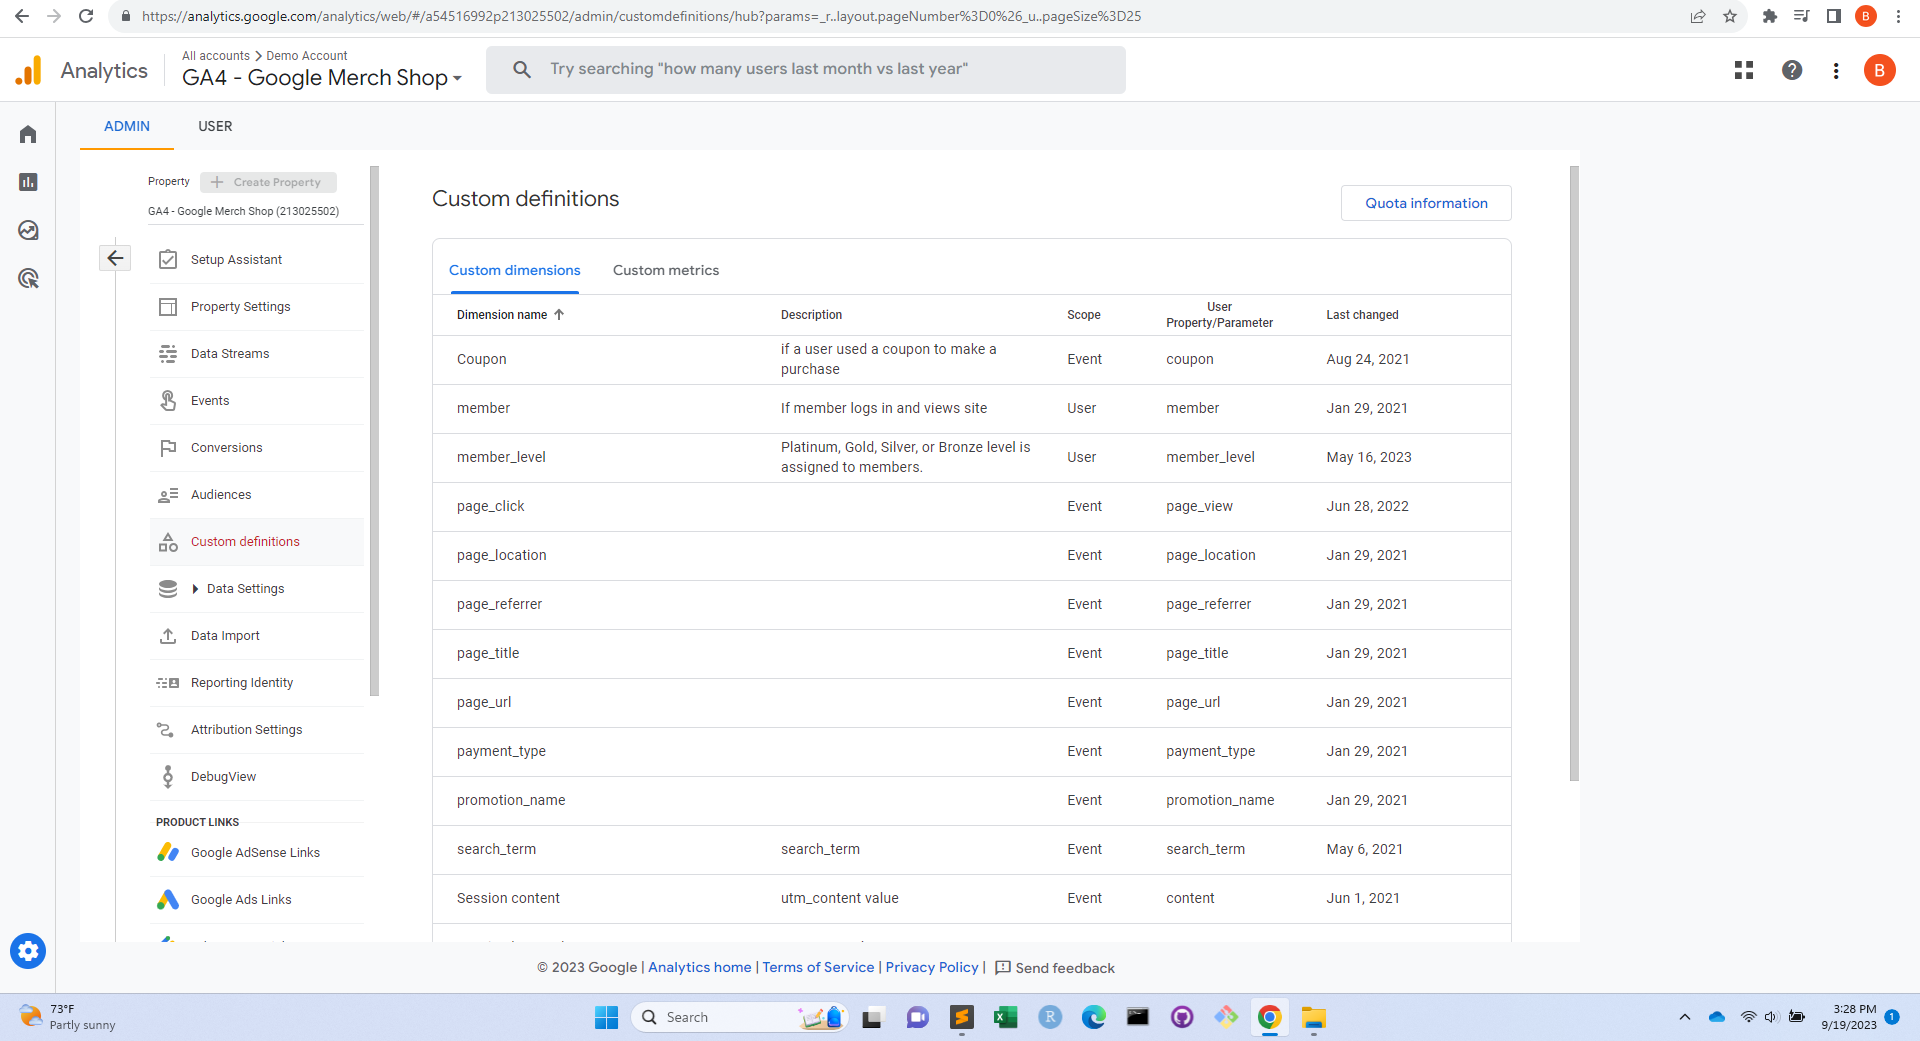
\includegraphics[height=5.6cm, trim=1.5cm 0.0cm 2.0cm 0.0cm width=5.6cm]{Images/G4A_7b_091923_Admin_Customdefinitions_Customdimensions.png}
  \caption{Figure {\color{franklinblue} 15}: GA4 \texttt{Admin} Custom Dimensions}
\end{figure}
\vspace{-2.0ex}
\small
Note a {\color{blue} create custom dimension} button is \underline{not} illustrated in the screenshot since we are \underline{not} one of the ``select GA4 end-users'' of the ``GA4 - Google Merch Shop'' property. 
\end{frame}

\begin{frame}[t]{GA4 \texttt{Admin} Custom Metrics}
\begin{figure}[htbp]
  \captionsetup{justification=centering}
  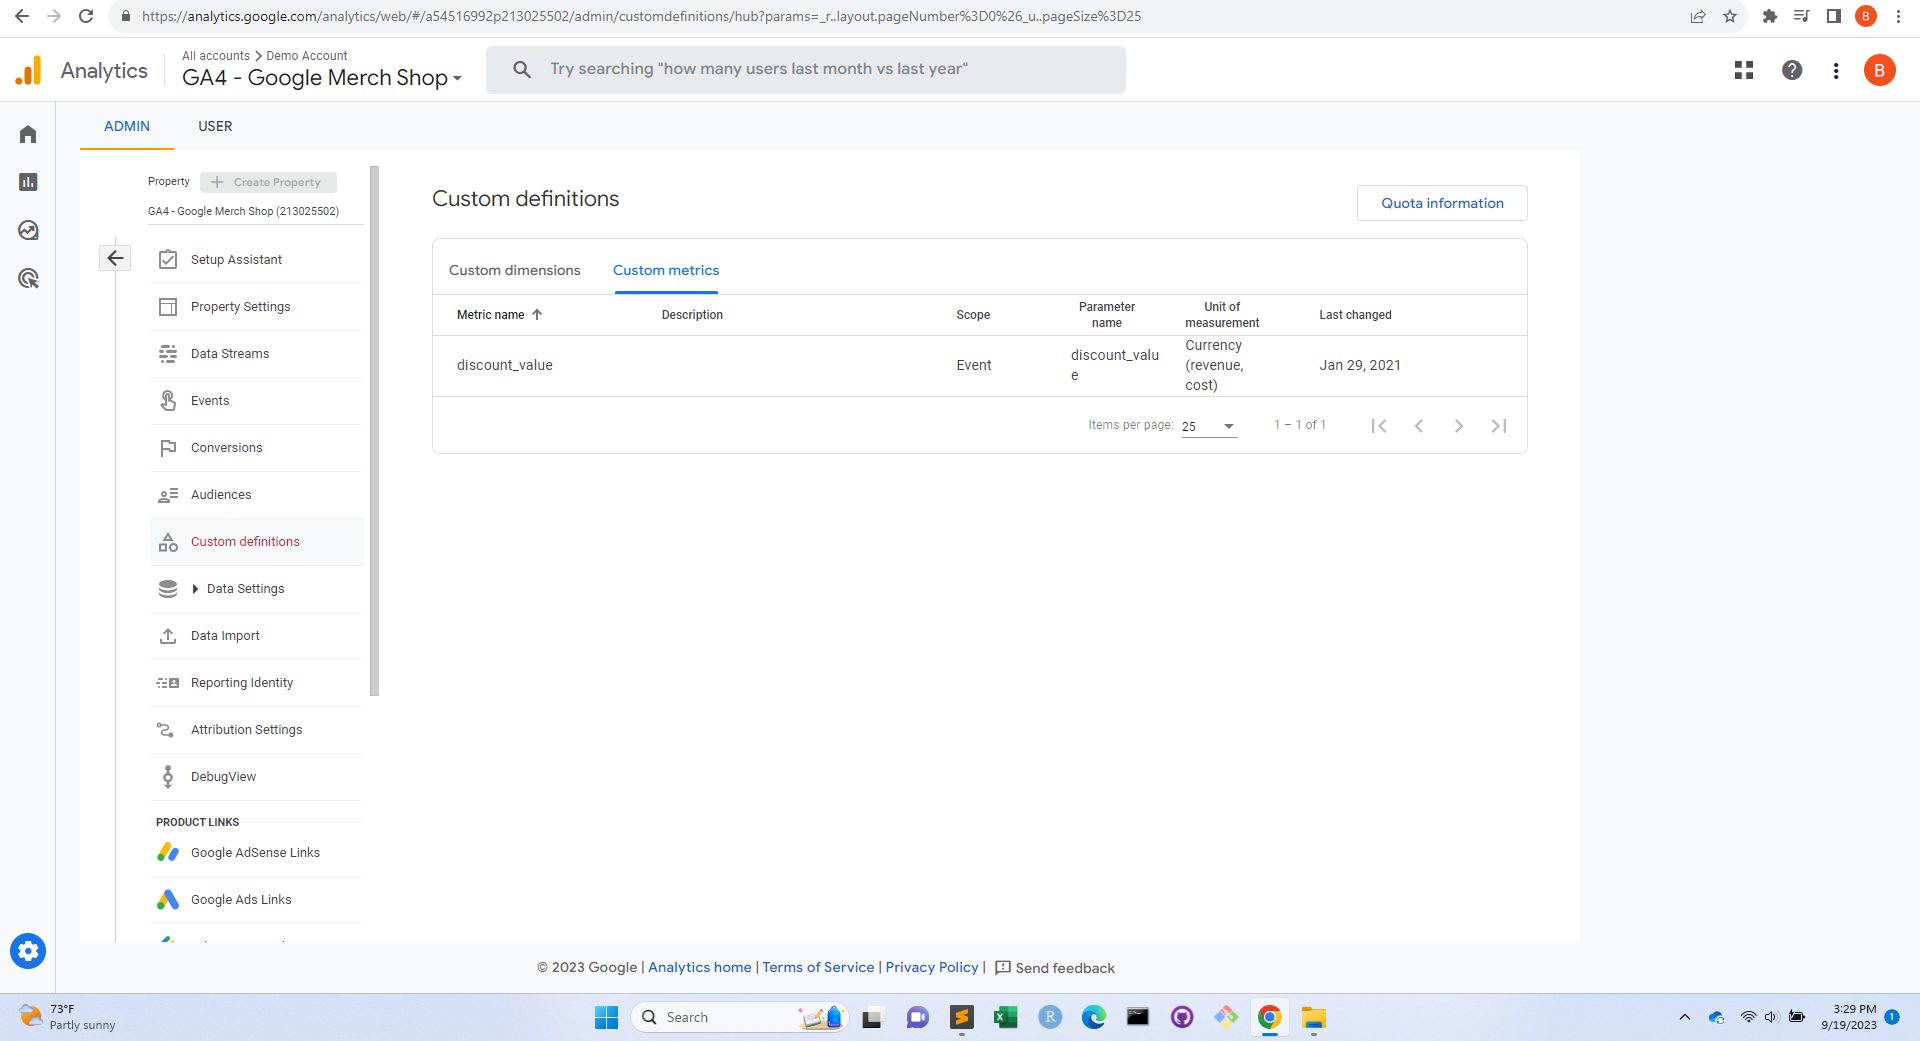
\includegraphics[height=5.6cm, trim=1.5cm 0.0cm 2.0cm 0.0cm width=5.6cm]{Images/G4A_7c_091923_Admin_Customdefinitions_Custommetrics.png}
  \caption{Figure {\color{franklinblue} 16}: GA4 \texttt{Admin} Custom Metrics}
\end{figure}
\vspace{-2.0ex}
\small
Note a  {\color{blue} create custom metric} button is \underline{not} illustrated in the screenshot since we are \underline{not} one of the ``select GA4 end-users'' of the property. 
\end{frame}

\begin{frame}[t]{Managing Account Access and Settings}
\small 
\begin{itemize}
  \item \textit{Administrators} have full control of the GA4 account. They can manage users (add or delete users, assign any role or data restriction) and grant full permissions to any user.
  \item \textit{Editors} have full control of the settings of the account and its properties. Editors cannot manage users.
  \item \textit{Marketers}  can create, edit, and delete \textit{audiences}, conversions, \textit{attribution models}, events, and \textit{lookback windows}.\footnote{(1) A GA4 audience is a group of site and/or app users who have generated similar behavioral data or who share demographic or other descriptive data (e.g., same age group, were acquired by the same campaign). (2) Attribution is the act of assigning credit for conversions to different ads, clicks, and factors along a user's conversion path. A GA4 attribution model can be a rule, a set of rules, or a data-driven algorithm that determines how conversion credit is assigned to conversion path touchpoints. (3) Google Ad Manager only records conversions for users who have previously seen or clicked on a Google Ad Manager ad within a period of time that one specifies, called a lookback window (lbw). There are two lbws, one for clicks and one for impressions. The lbws are set for each activity group, and can be from 1 to 30 days.}
\end{itemize}
\end{frame}

\begin{frame}[t]{Managing Account Access and Settings Continued}
\small
\begin{itemize}
  \item \textit{Analysts} can create, edit, and delete certain property assets, like \textit{explorations}. They can also collaborate on shared assets.\footnote{Explorations are private by default. The creator of an exploration can share it with others.} 
  \item  \textit{Viewers} can see settings and data, and they can change the data they see in reports, like adding comparisons or adding a secondary dimension. Viewers can see new reports and collections in the left navigation, but they can't make changes to the navigation.
  \item Those who are classified as \textit{None} are people who have no role for the account or property, but may have a role for a \underline{related} account or property.
\end{itemize}
For the remainder of this section we will review a few GA4 reports that are frequently used.  As you will discover during the tutorials, these reports are just a small subset of those provided by GA4.
\end{frame}

\begin{frame}[t]{GA4 \texttt{Home Page} Insights}
%https://support.google.com/analytics/answer/11197963?hl=en
The \texttt{Home Page} surfaces information that is relevant to an organization. \\
\vspace{1.5ex}
One can use the page to monitor traffic, navigate around GA4, and get insights about the organization's websites and mobile apps. \\
\vspace{1.5ex}
The \texttt{Overview} \textit{card} shows metrics that are relevant with a trendline for each metric. \\
\small
\begin{itemize}
\item Cards focus on a specific objective. 
\item These cards are typically previews of a detail report, which lets one dig deeper into the data set. 
\end{itemize} 
\end{frame}

\begin{frame}[t]{GA4 \texttt{Home Page}}
\begin{figure}[htbp]
  \captionsetup{justification=centering}
  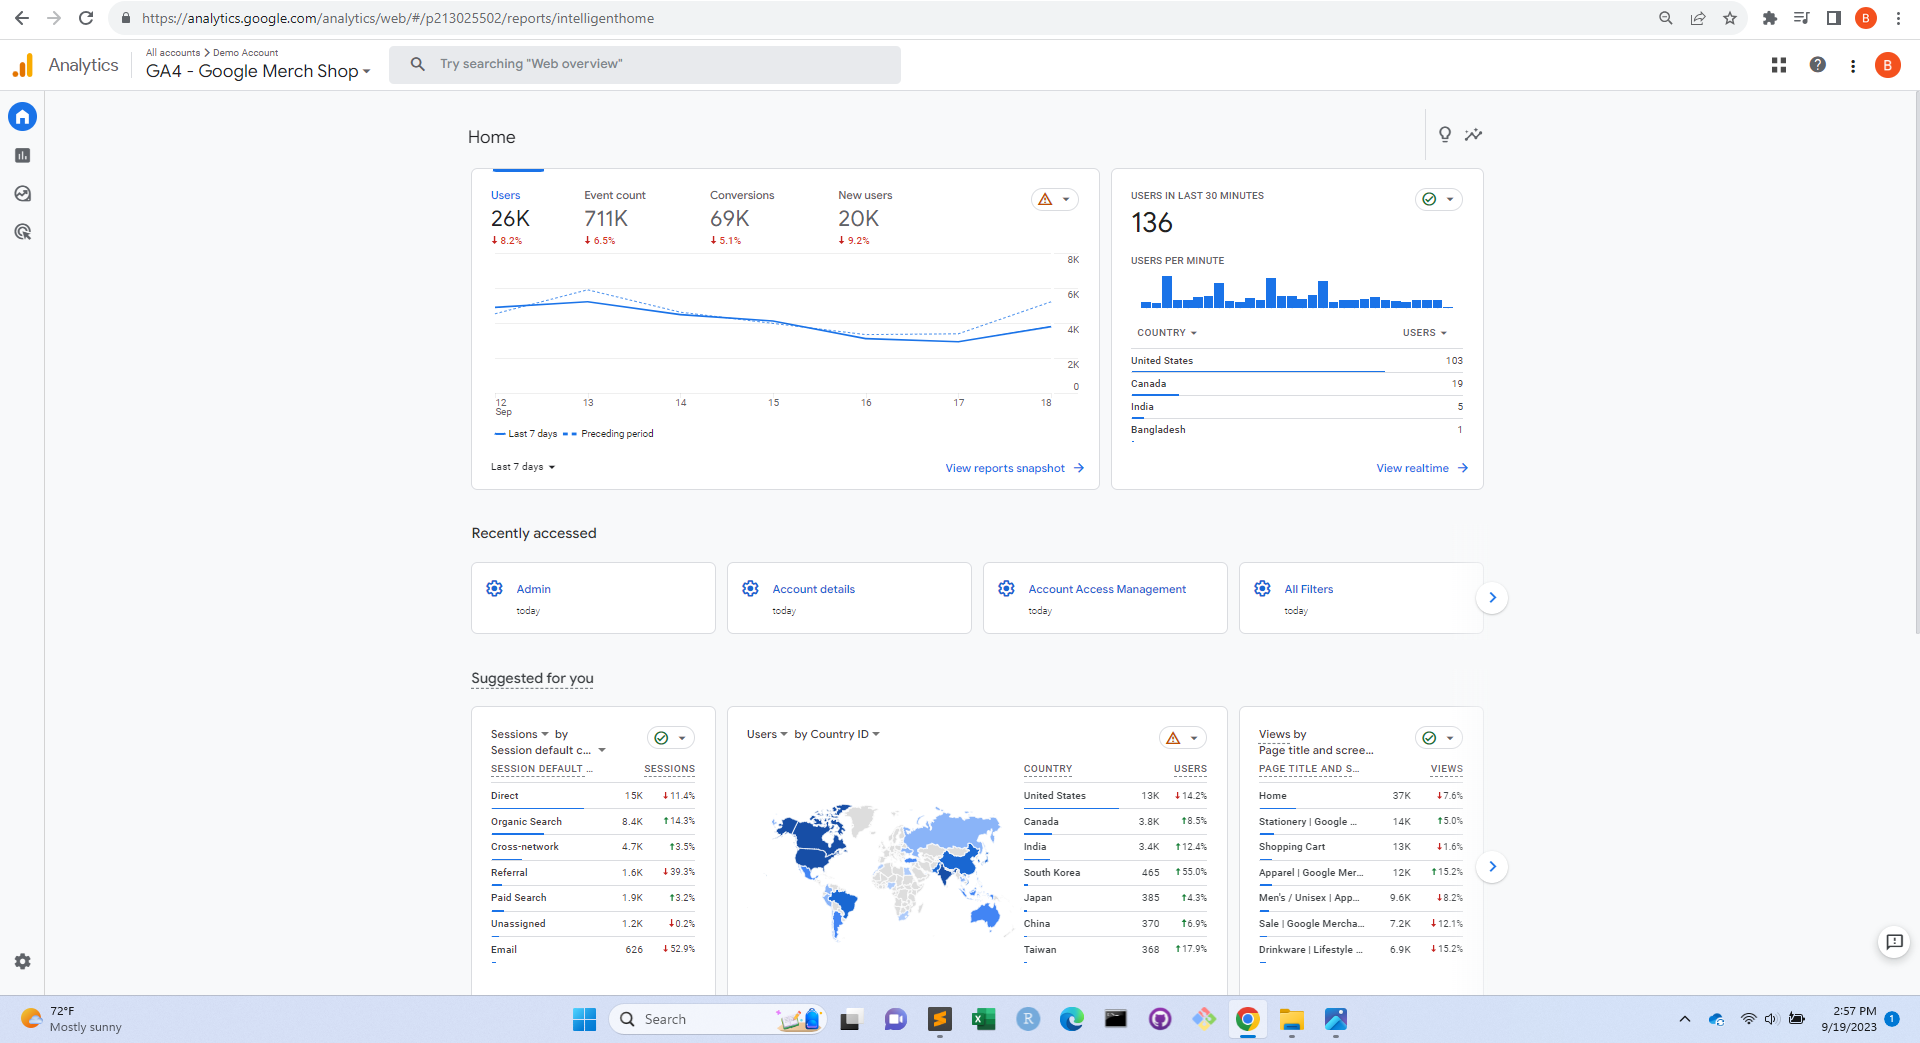
\includegraphics[height=5.6cm, trim=1.5cm 0.0cm 2.0cm 0.0cm width=5.6cm]{Images/G4A_6a_091923_Homepage_and_Search_Bar.png}
  \caption{Figure {\color{franklinblue} 17}: GA4 \texttt{Home Page}}
\end{figure}
\end{frame}

\begin{frame}[t]{Card Controls and Search Box}
Card controls include: \\
\vspace{0.5ex}
\small
\begin{itemize}
\item Dimension/metric picker: If a card has dimension or metric pickers across the top, one can use them to change which data is displayed in the card. 
\item Date range selector: One can use the date range selector in the upper right to select the time frame for reporting. 
\item Link to associated report: To open the associated report, select the link at the bottom right of the card. This will open a more in-depth report on the card topic.
\end{itemize}
\normalsize
To find a specific report or insight use the \textit{search box} at the top of the GA4 account to ask a question, such as,  ``How many people came to the website last month?'' When one selects the search box, they will see recent searches and reports opened, as well as suggested queries.
\end{frame}

\begin{frame}[t]{GA4 \texttt{Realtime} Report}
% https://support.google.com/analytics/answer/9271392?sjid=2669540208995570408-NA
\texttt{Realtime} lets one monitor activity on the website or app as it happens. %The arrangement of cards lets one see how users enter the conversion funnel, and how they behave once they are in the funnel.
\begin{figure}[htbp]
  \captionsetup{justification=centering}
  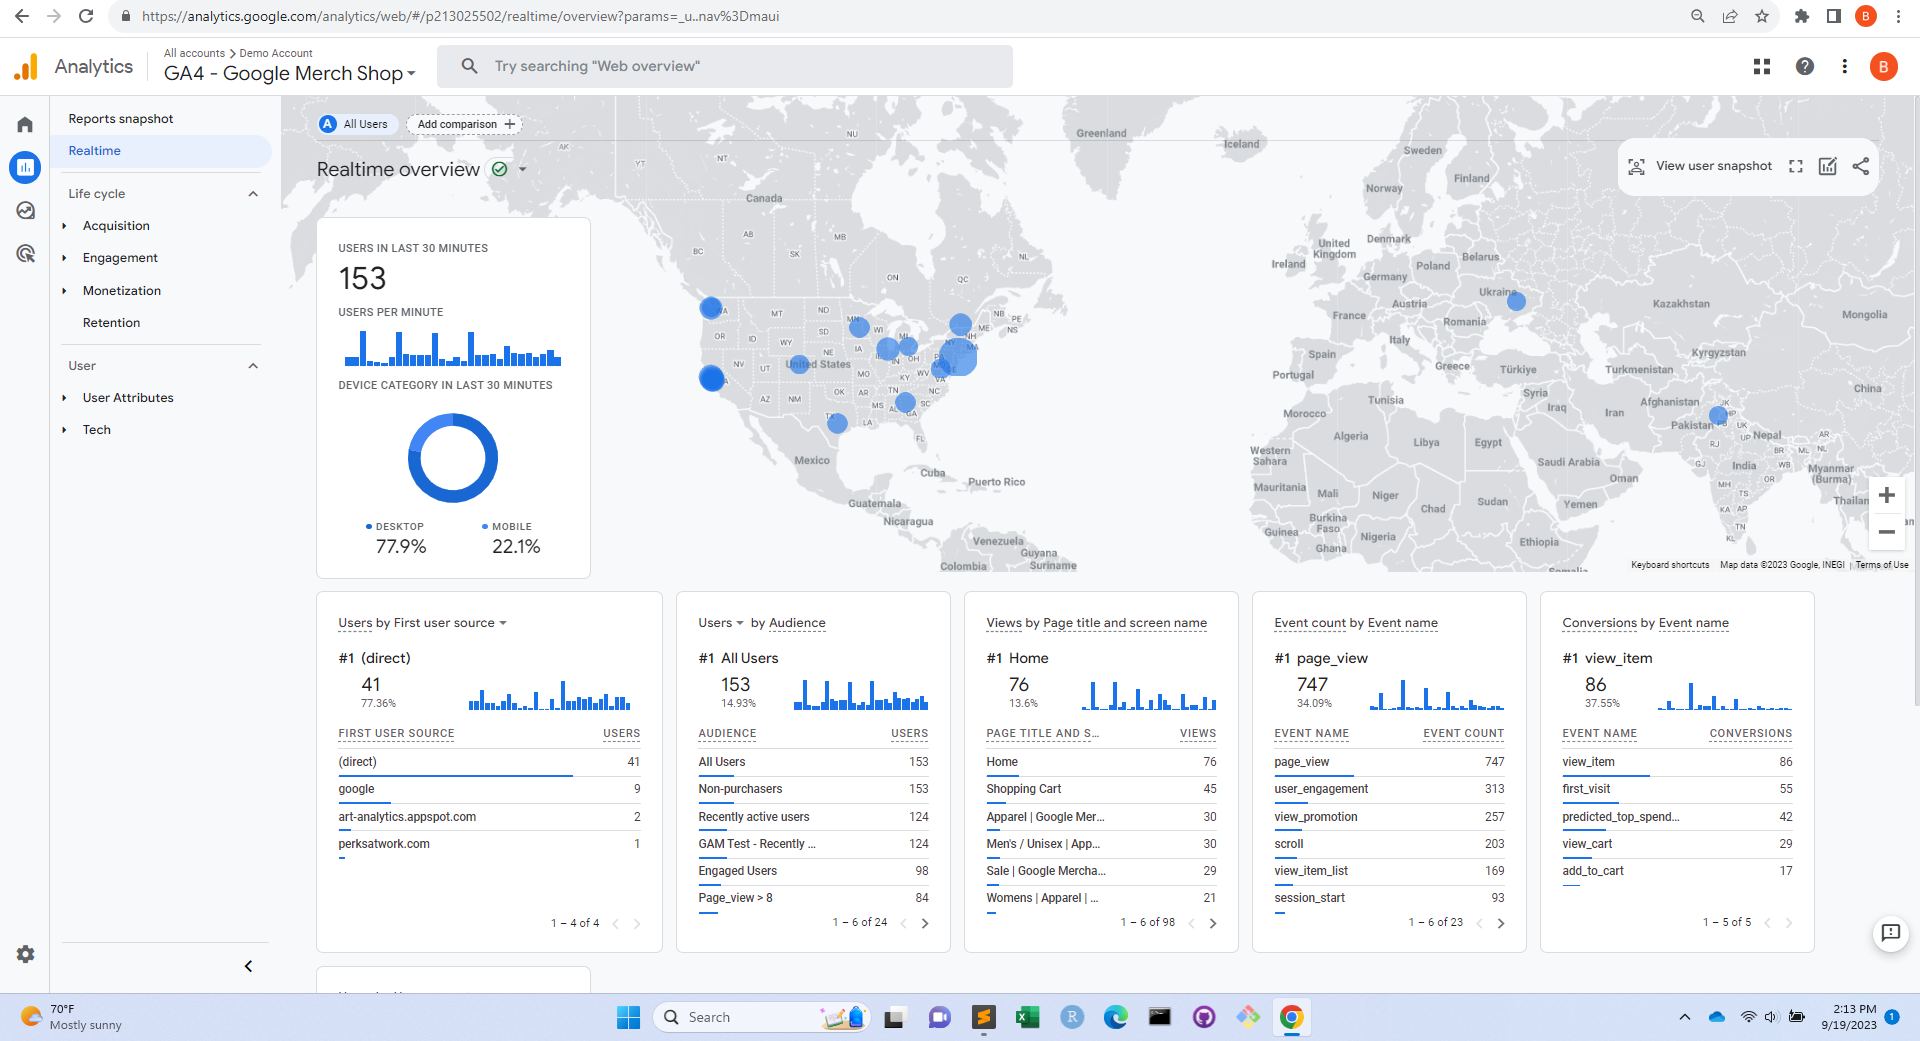
\includegraphics[height=5.6cm, trim=1.5cm 0.0cm 2.0cm 0.0cm width=5.6cm]{Images/GA4_3_091923_Realtime_Reports.png}
  \caption{Figure {\color{franklinblue} 18}: GA4 \texttt{Realtime} Report}
\end{figure}
\end{frame}

\begin{frame}[t]{GA4 \texttt{Realtime} Report Insights}
\small
\texttt{Realtime} lets one see: \\
\begin{itemize}
\item 'Users in Last 30 Minutes', which shows all users on the organization's site or app.
\item 'New users', which shows users on the organization's site or app for the first time.
\item 'Users', which shows returning users.
\end{itemize}
With \texttt{Realtime}, one can immediately and continuously monitor the effects that new campaigns and site changes have on traffic. \\
\begin{itemize}
\item See whether a one-day promotion is driving traffic to the site or app.
\item Monitor the immediate effects on traffic from a blog/social network post or tweet.
\item Monitor whether new and changed content on the site is affecting traffic.  In addition, verify that the measurement code is working on the site or app.
\end{itemize}
\end{frame}

\begin{frame}[t]{GA4 \texttt{Reports snapshot}}
\begin{figure}[htbp]
  \captionsetup{justification=centering}
  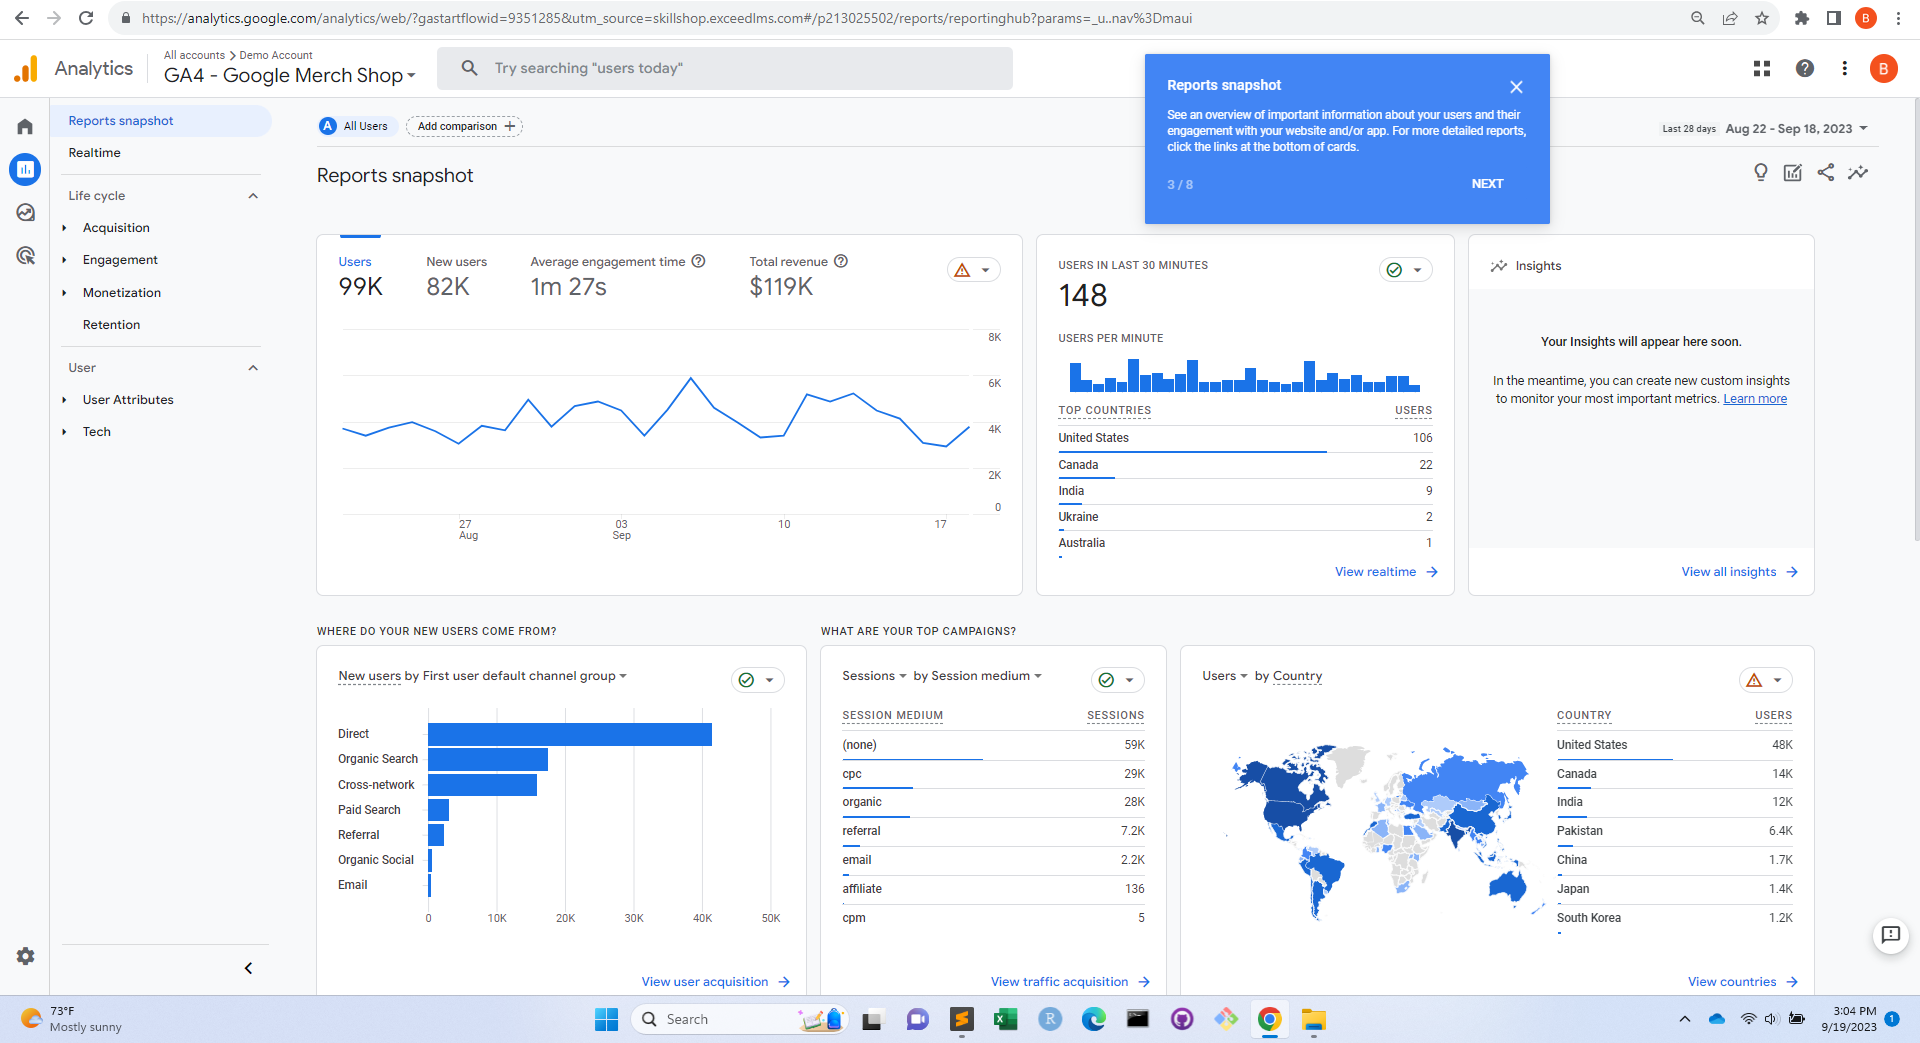
\includegraphics[height=5.6cm, trim=1.5cm 0.0cm 2.0cm 0.0cm width=5.6cm]{Images/G4A_6b_091923_Reports_Snapshot.png}
  \caption{Figure {\color{franklinblue} 19}: GA4 \texttt{Reports snapshot}}
\end{figure}
\vspace{-2.0ex}
\small 
The \texttt{Reports snapshot} is the overview report displayed when one clicks \texttt{Reports} in the left navigation. Any overview report can be set as the \texttt{Reports} snapshot.
\end{frame}

\begin{frame}[t]{GA4 \texttt{Reports} Sections}
\begin{figure}[htbp]
  \captionsetup{justification=centering}
  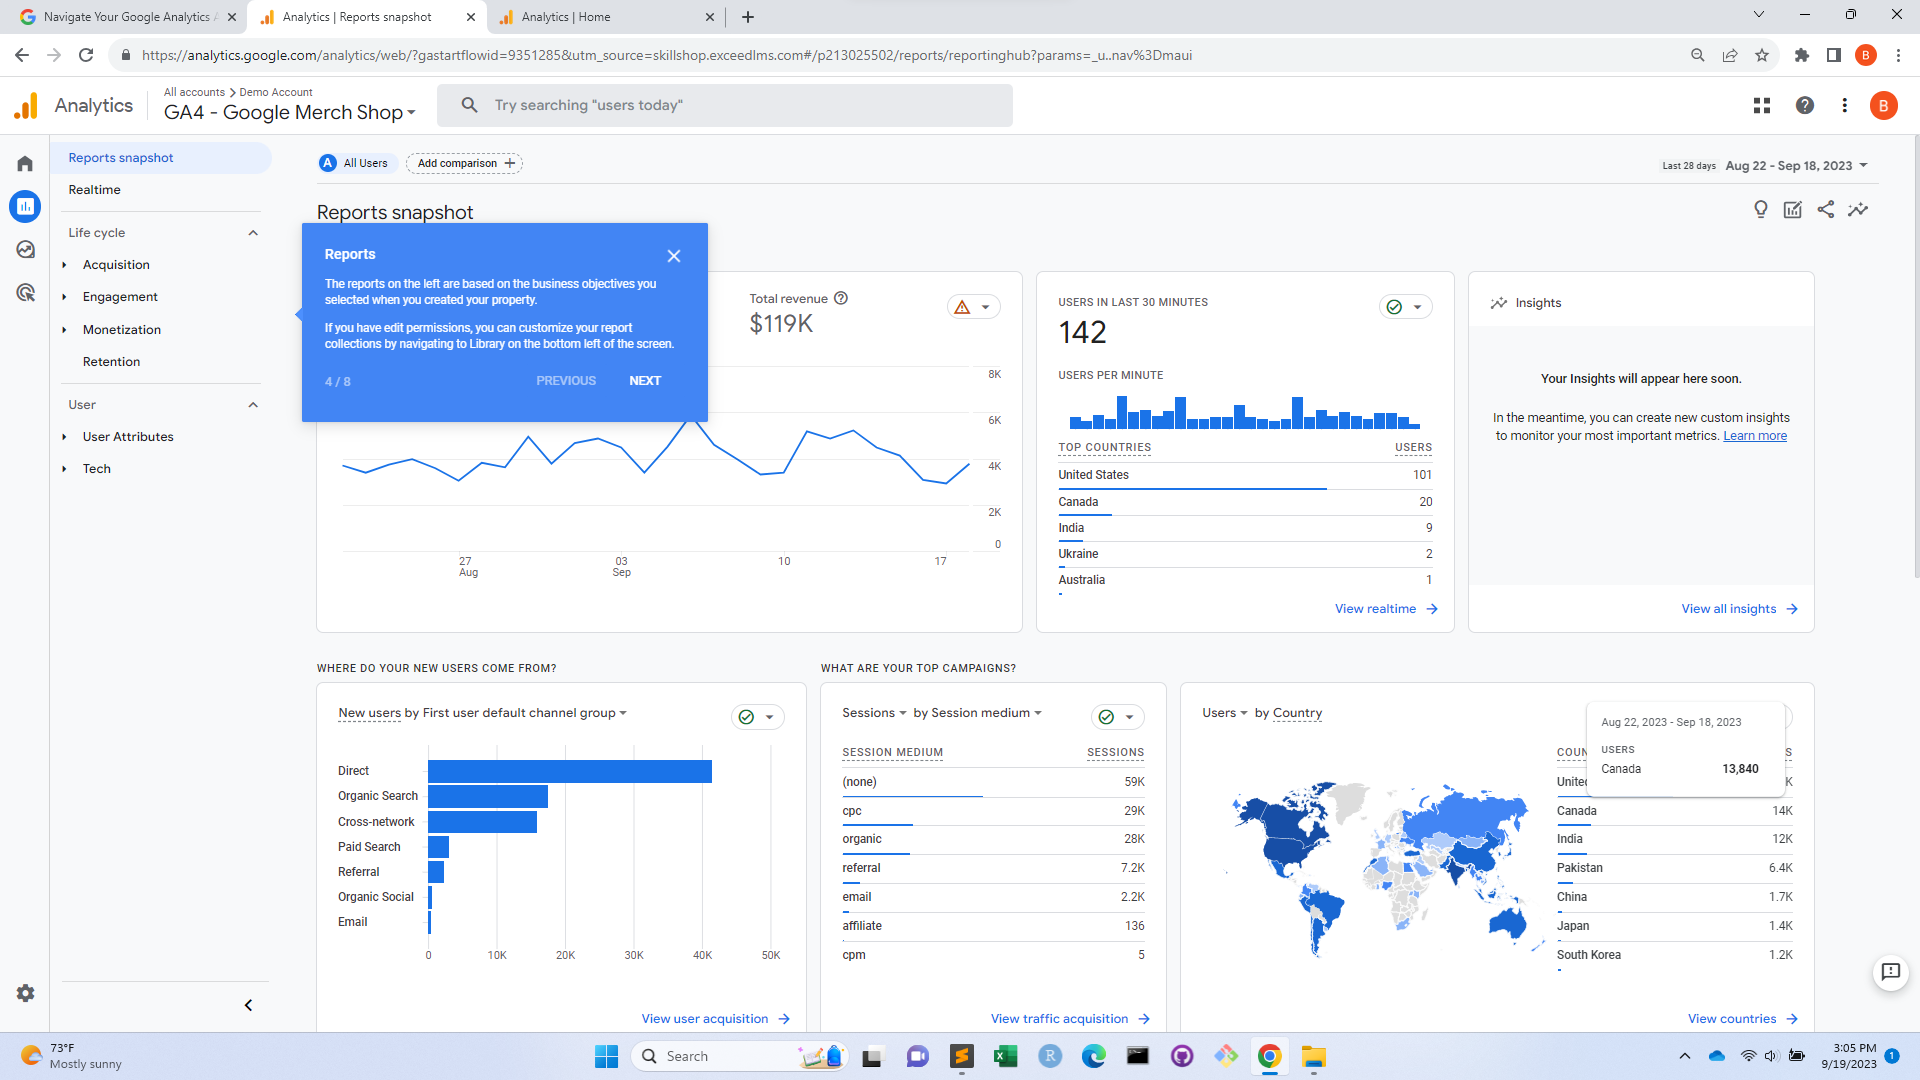
\includegraphics[height=5.6cm, trim=1.5cm 0.0cm 2.0cm 0.0cm width=5.6cm]{Images/G4A_6c_091923_Reports.png}
  \caption{Figure {\color{franklinblue} 20}: GA4 \texttt{Reports} Sections}
\end{figure}
\vspace{-2.0ex}
\small 
 The \textit{Reports} section allows one to view ready-made reports that answer common questions about how users are interacting with the app or website.
\end{frame}

\begin{frame}[t]{GA4 \texttt{Acquisition Overview} Report}
\begin{figure}[htbp]
  \captionsetup{justification=centering}
  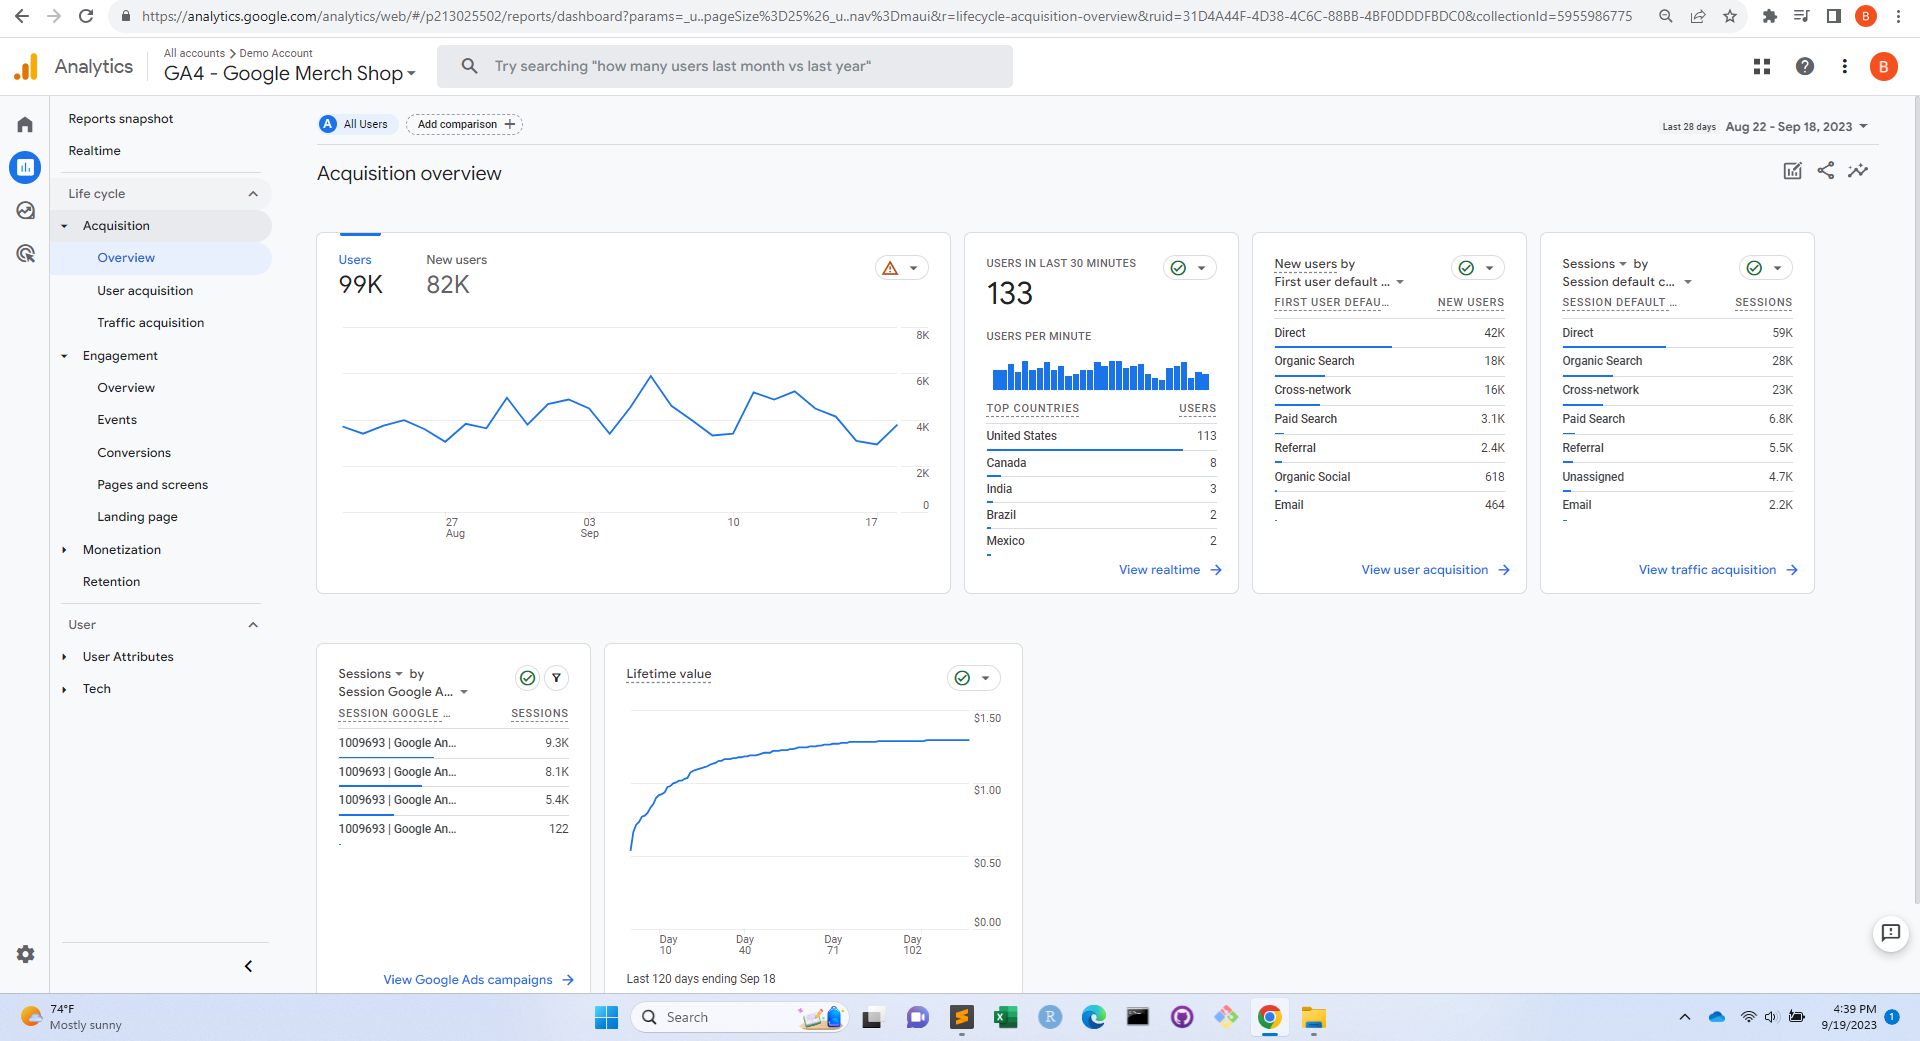
\includegraphics[height=5.6cm, trim=1.5cm 0.0cm 2.0cm 0.0cm width=5.6cm]{Images/G4A_8a_091923_Acquisition_Overview.png}
  \caption{Figure {\color{franklinblue} 21}: GA4 \texttt{Acquisition Overview} Report}
\end{figure}
\vspace{-2.0ex}
\small 
%https://support.google.com/analytics/answer/13410671?hl=en&ref_topic=13818299&sjid=544685887880557031-NA
% This pre-made overview report summarizes the acquisition data. 
This pre-made report can help determine if marketing is attracting new website or app users, if re-engagement campaigns are bringing users back, and if marketing strategies should continue or be adjusted.
\end{frame}

\begin{frame}[t]{GA4 \texttt{Engagement Overview} Report}
\begin{figure}[htbp]
  \captionsetup{justification=centering}
  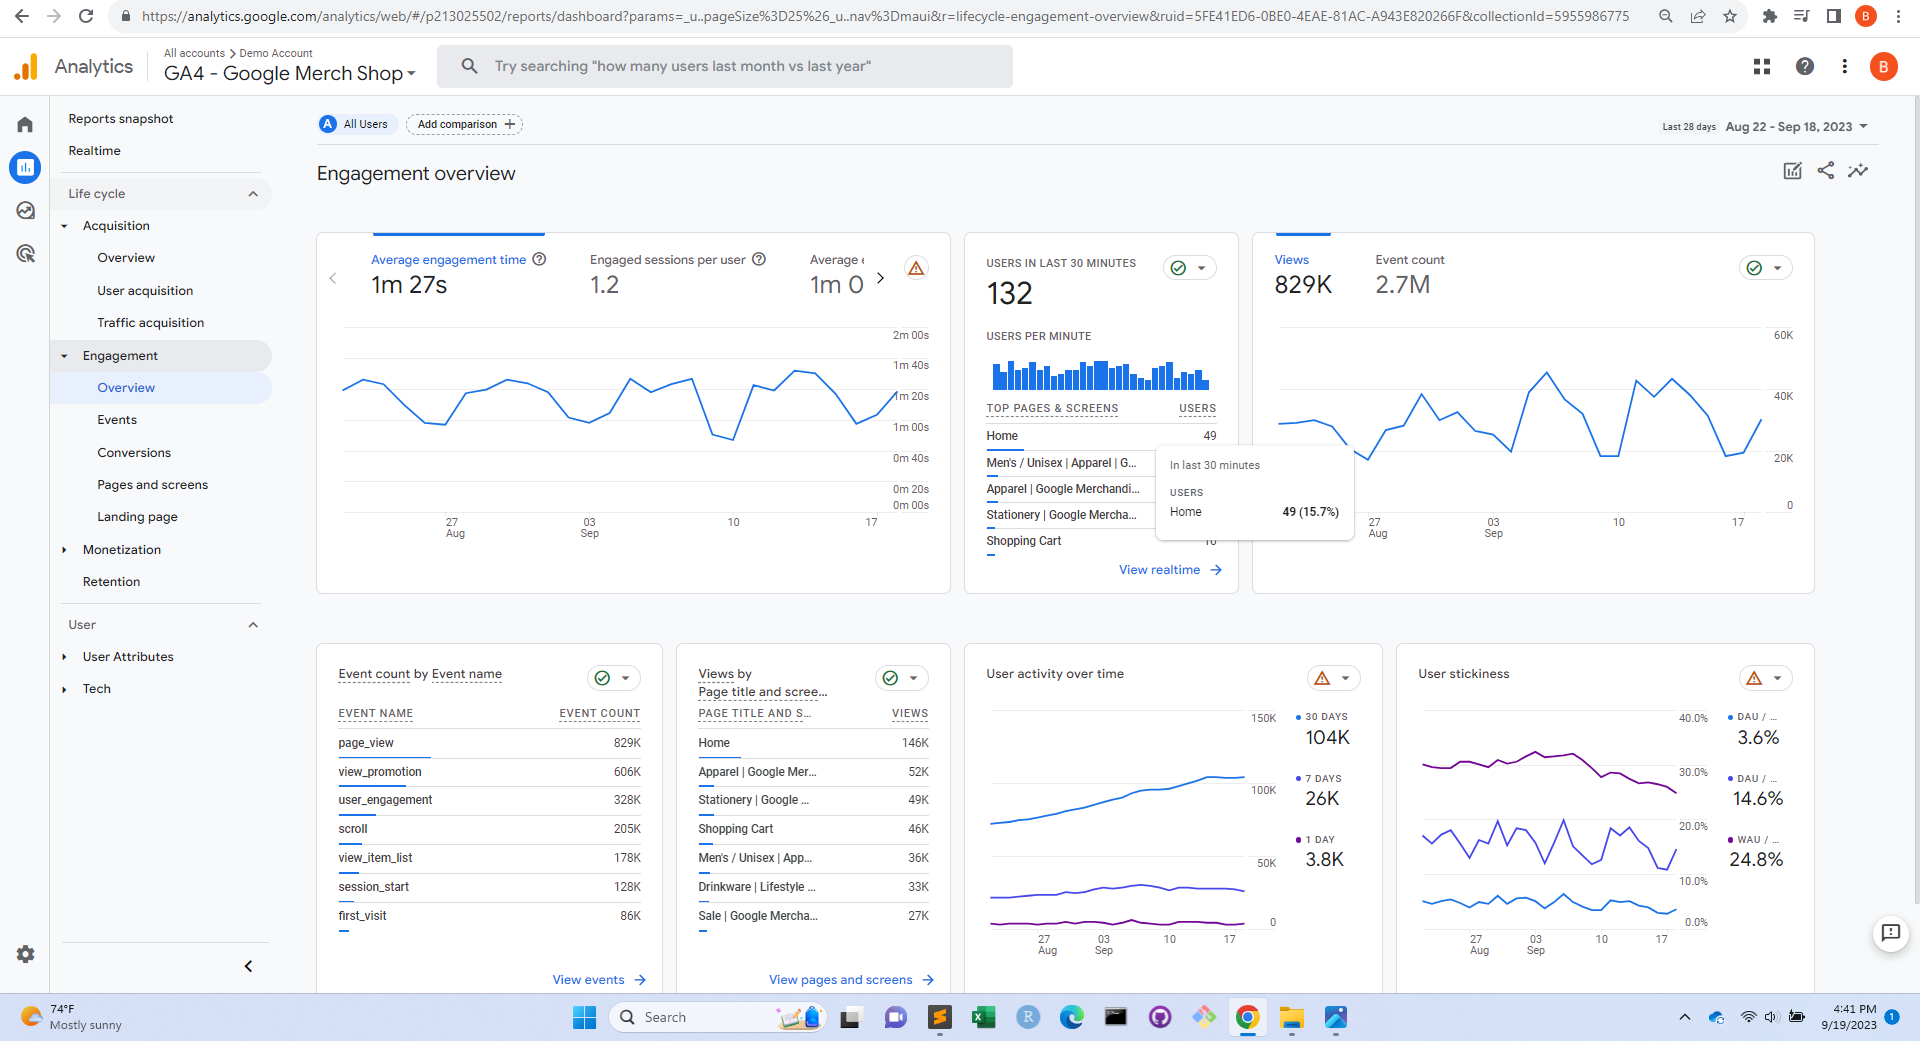
\includegraphics[height=5.6cm, trim=1.5cm 0.0cm 2.0cm 0.0cm width=5.6cm]{Images/G4A_8b_091923_Engagement_Overview.png}
  \caption{Figure {\color{franklinblue} 22}: GA4 \texttt{Engagement Overview} Report}
\end{figure}
\vspace{-2.0ex}
\small 
% https://support.google.com/analytics/answer/13391283?hl=en&ref_topic=13818299&sjid=544685887880557031-NA
% This pre-made report summarizes the engagement data. 
This pre-made report can be used to compare key engagement metrics over time, understand which pages and screens users are visiting, and identify the features with which they are interacting.
\end{frame}

\begin{frame}[t]{GA4 \texttt{Monetization Overview} Report}
\begin{figure}[htbp]
  \captionsetup{justification=centering}
  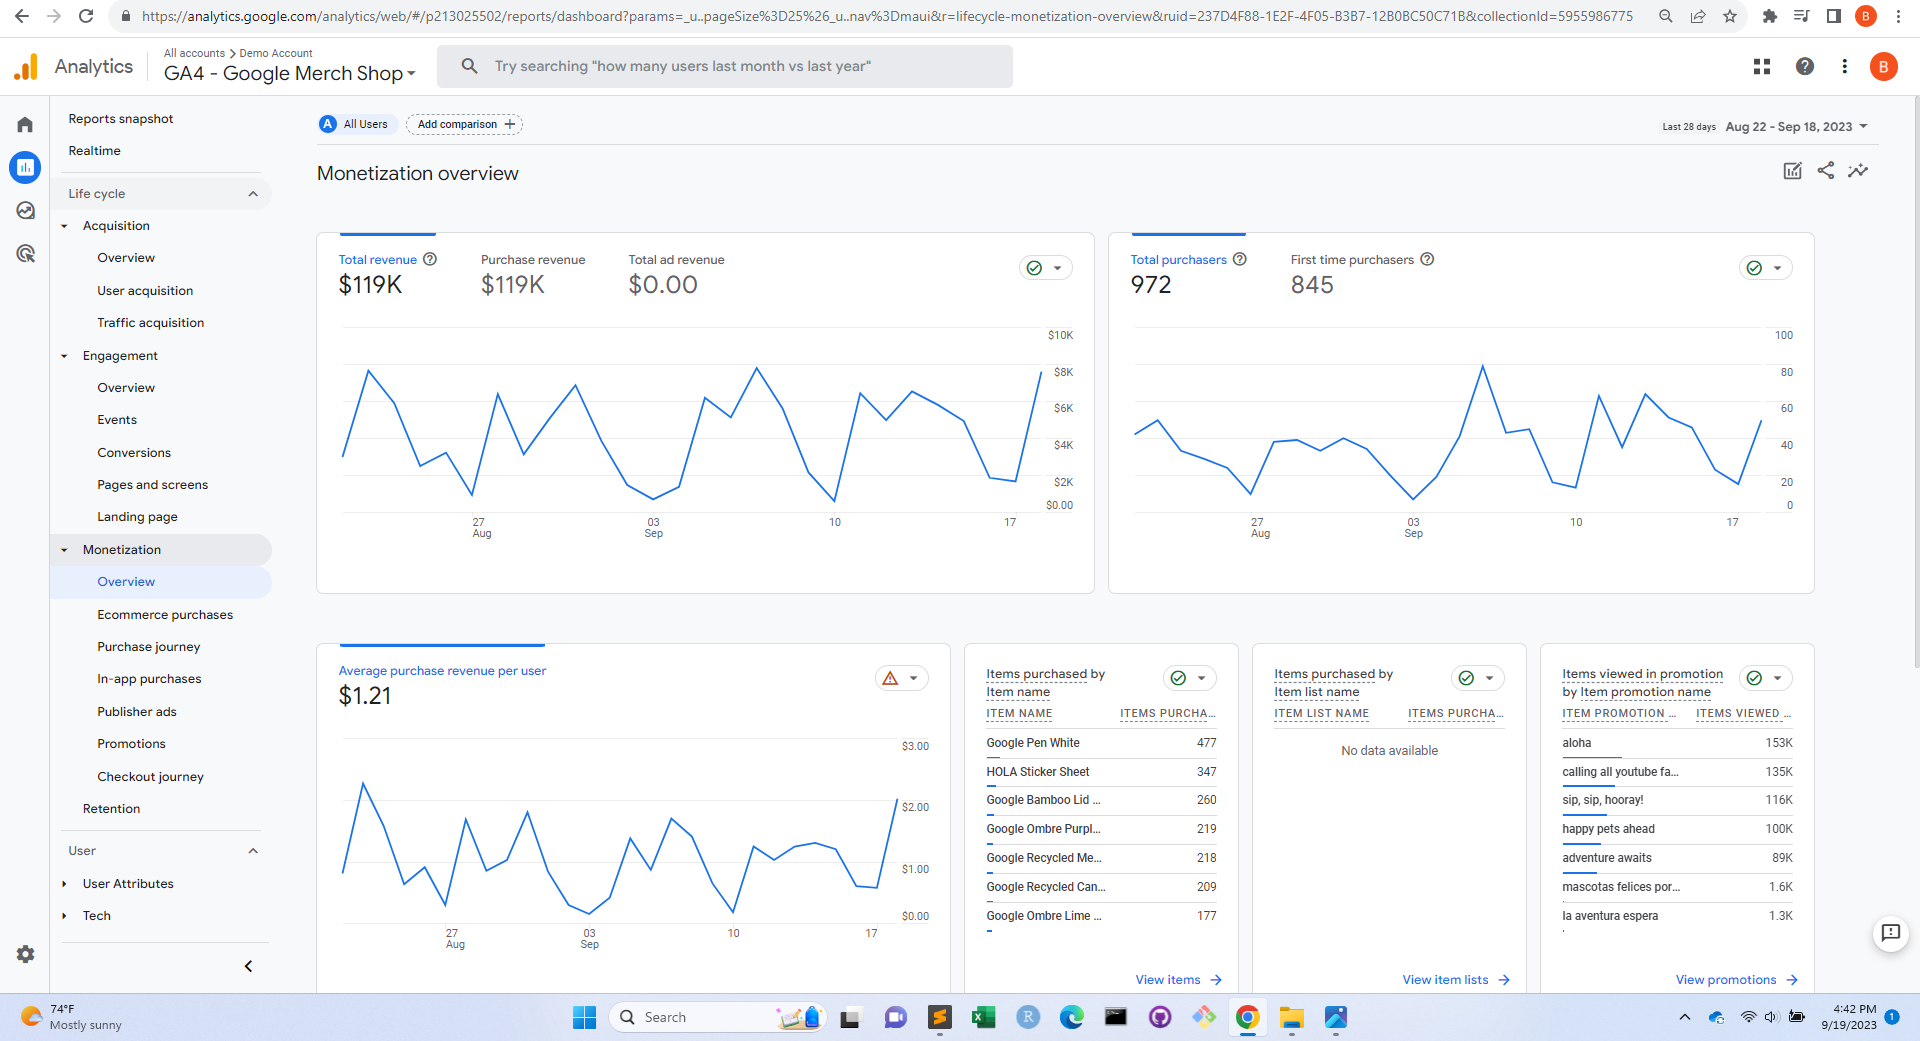
\includegraphics[height=5.6cm, trim=1.5cm 0.0cm 2.0cm 0.0cm width=5.6cm]{Images/G4A_8c_091923_Monetization_Overview.png}
  \caption{Figure {\color{franklinblue} 23}: GA4 \texttt{Monetization Overview} Report}
\end{figure}
\vspace{-2.0ex}
\small 
%This pre-made report summarizes revenue data. 
This pre-made report can help determine which products are selling, if promotions and coupons are successfully bringing in new users, and if ads displayed on the mobile app yield revenue.
\end{frame}

\begin{frame}[t]{GA4 \texttt{Explorations} Section}
\begin{figure}[htbp]
  \captionsetup{justification=centering}
  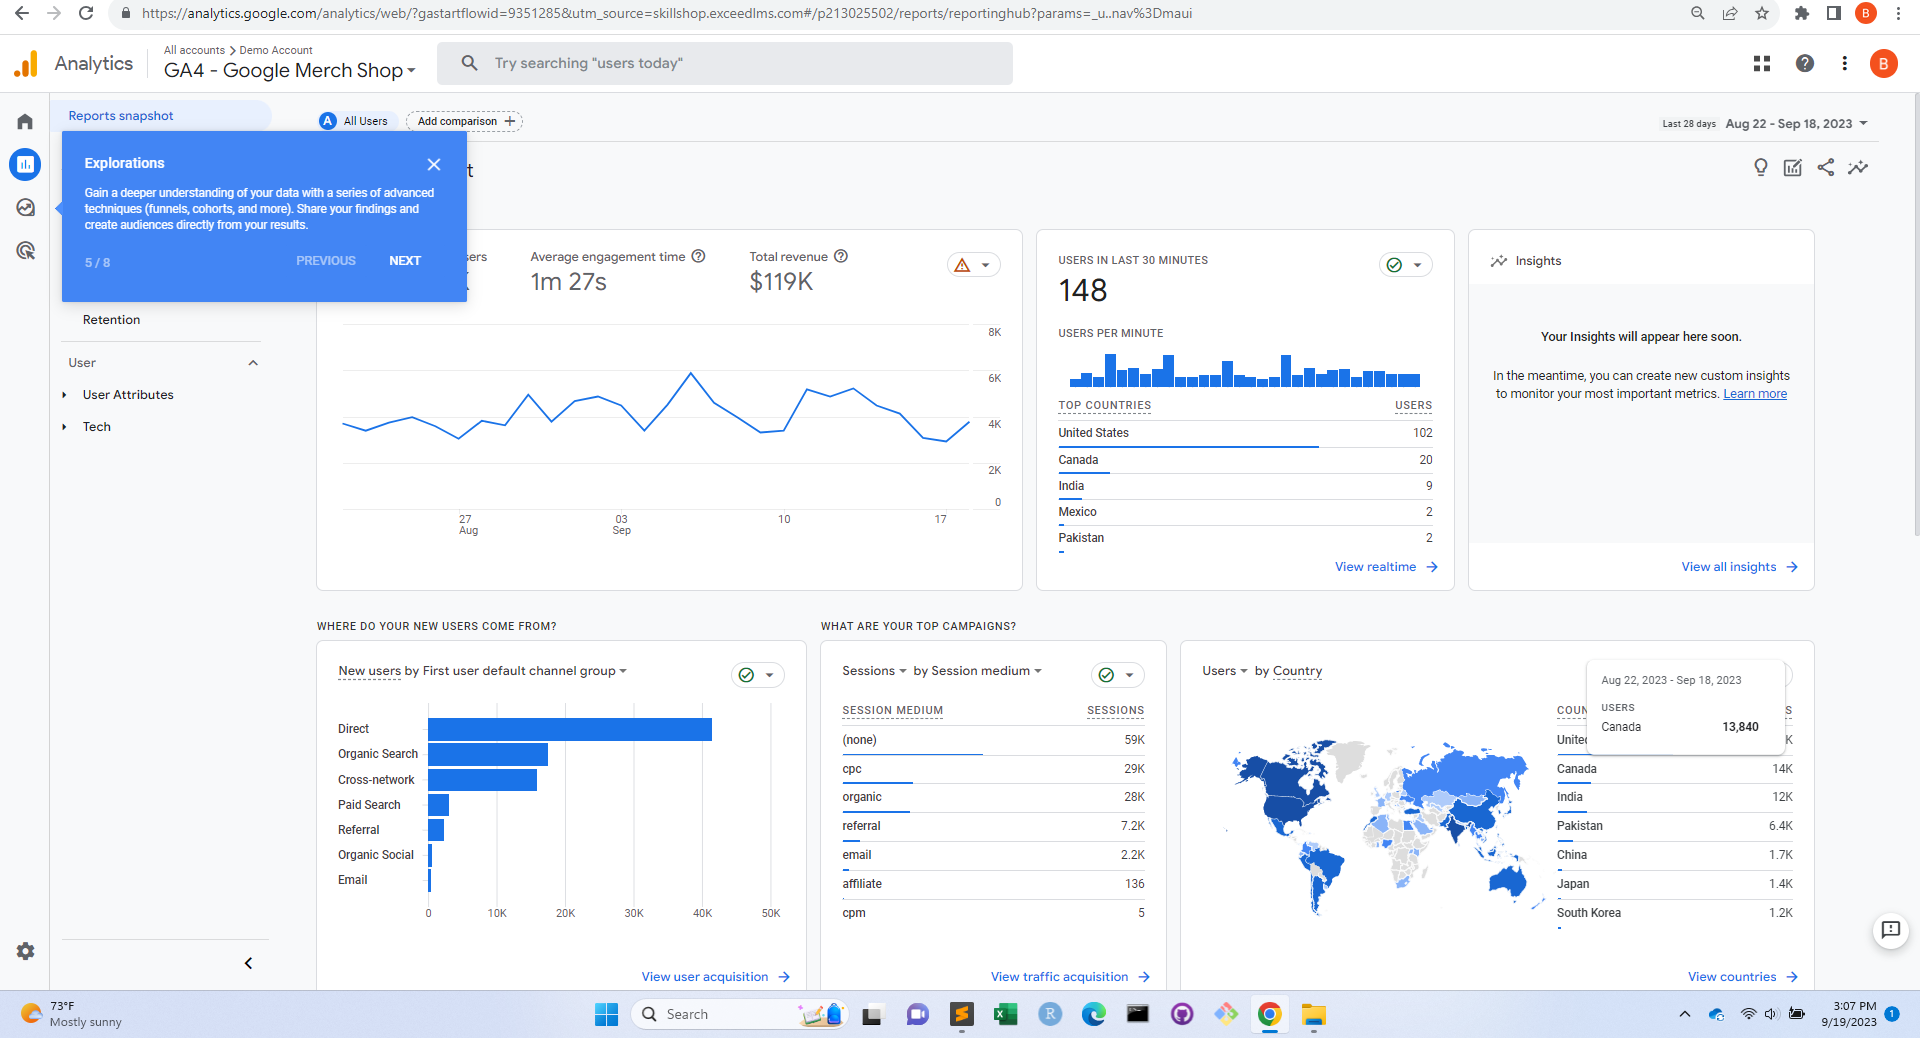
\includegraphics[height=5.6cm, trim=1.5cm 0.0cm 2.0cm 0.0cm width=5.6cm]{Images/G4A_6d_091923_Explorations.png}
  \caption{Figure {\color{franklinblue} 24}: GA4 \texttt{Explorations} Section}
\end{figure}
\vspace{-2.0ex}
\small 
% https://support.google.com/analytics/answer/7579450?hl=en#zippy=%2Cin-this-article
\texttt{Explorations} is a collection of advanced techniques that go beyond standard reports to help an organization uncover deeper insights about user behavior.
\end{frame}

\begin{frame}[t]{GA4 \texttt{Advertising} Section}
\begin{figure}[htbp]
  \captionsetup{justification=centering}
  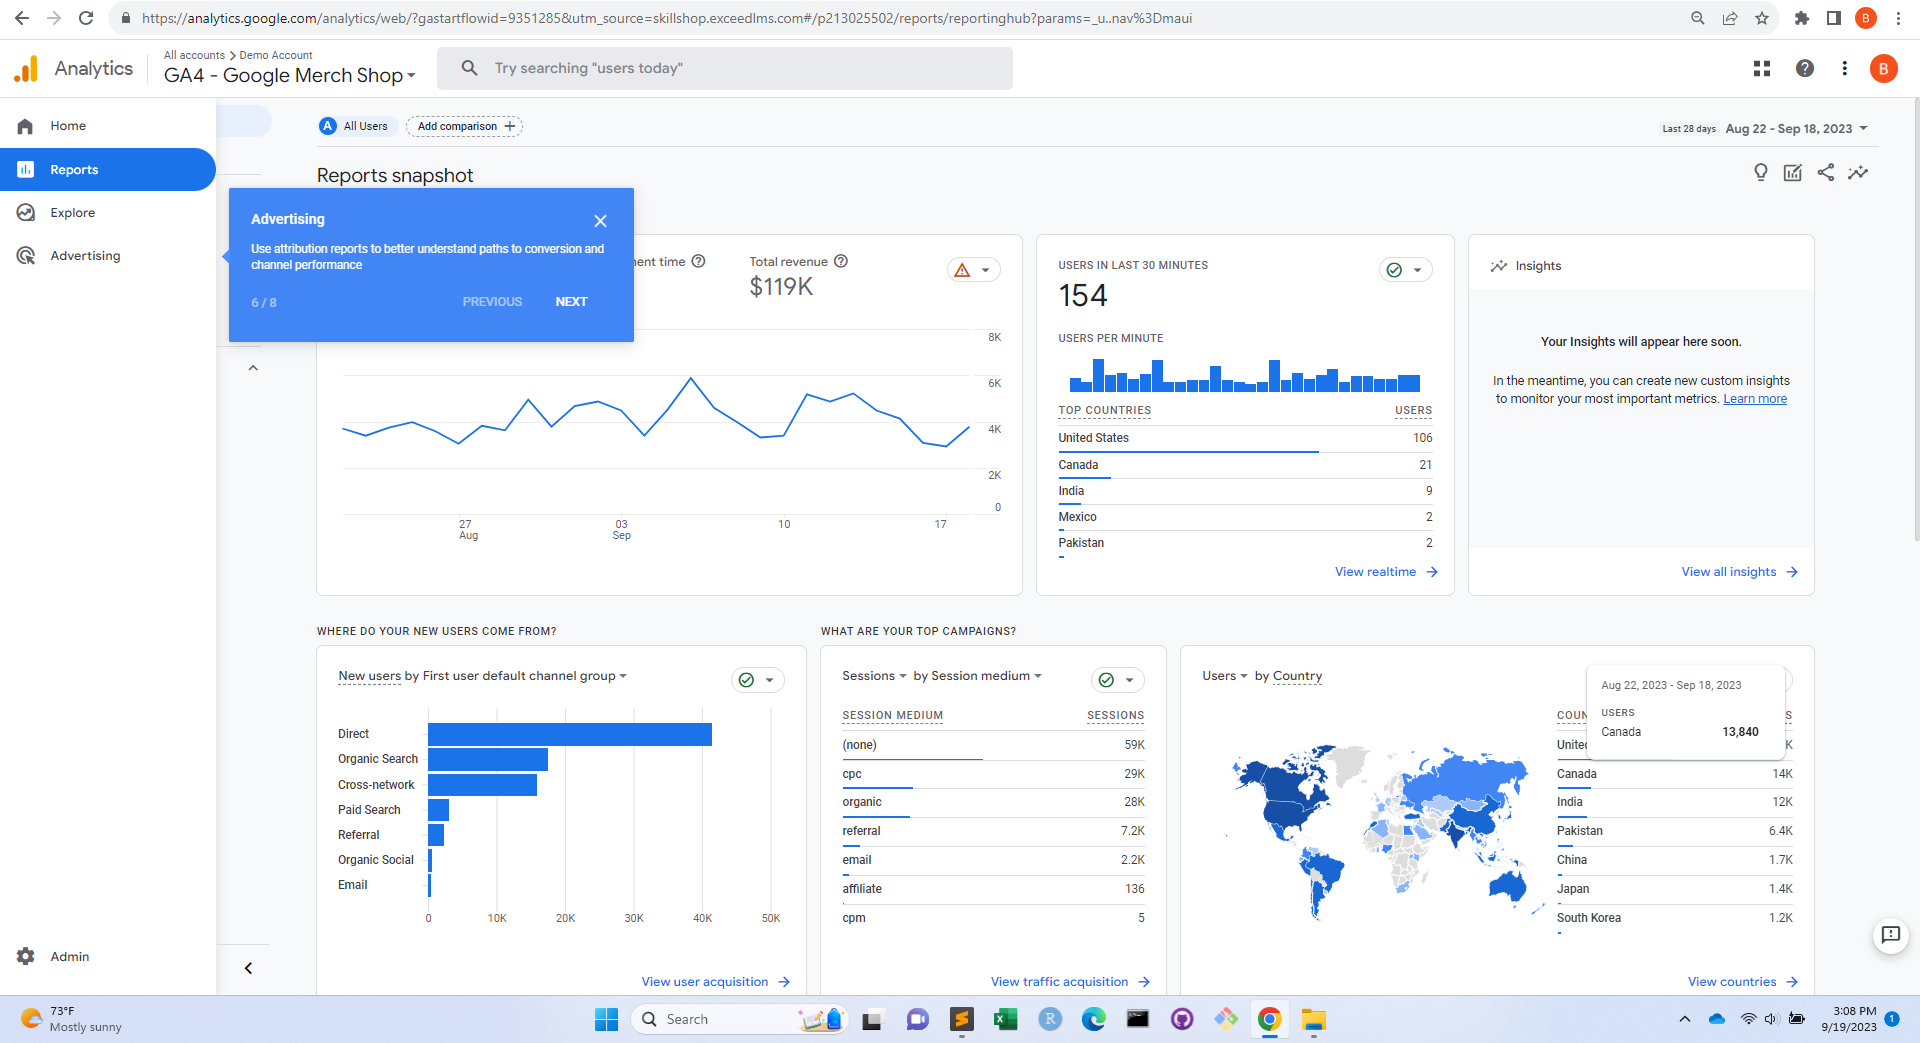
\includegraphics[height=5.6cm, trim=1.5cm 0.0cm 2.0cm 0.0cm width=5.6cm]{Images/G4A_6f_091923_Advertising.png}
  \caption{Figure {\color{franklinblue} 25}: GA4 \texttt{Advertising} Section}
\end{figure}
\vspace{-2.0ex}
\small 
% Use the GA4 \texttt{Advertising} section of the property to get more insight into the most important user journeys. 
The reports in this section help one better understand the media ROI across all channels, make informed decisions about budget allocation, and evaluate attribution models.
\end{frame}

\section{Content Analysis Tools}

\begin{frame}[t]{Comparing Content Analysis \& Social Listening Tools}
Content analysis tools allow marketing analytics professionals to analyze digital text, photos, audio, or visual formats of communication in greater detail than social listening tools. \\
\vspace{1.5ex}
\begin{itemize}
\item Social listening tools generally provide broad analyses to monitor conversations on Instagram, Twitter, and Facebook in real time. 
\item Firms use content analysis tools to provide deep analyses on words or phrases that are associated with specific images posted on social media. Content analysis tools typically include both (1) \empr{sentiment analysis}, which focuses on translating words into customers' attitudes, and (2) \empr{text analysis}, which focuses more on general themes.
\end{itemize}
\end{frame}

\begin{frame}[t]{Commercial Content Analysis Tools}
\href{https://www.liwc.app/}{Linguistic Inquiry and Word Count} (LIWC), %pronounced “Luke”) 
is one of several content analysis commercial tools. \\
\vspace{1.5ex}
It interprets text to reveal the thoughts, attitudes, feelings, personality, and motivations of the author. 
\begin{itemize}
%How does it work? 
\item It has decades-worth of built-in dictionaries that translate words and phrases into psychological states (e.g., irony, sarcasm, metaphor, \ldots).  More specifically, LIWC uses statistical supervised learners to attribute words to psychological states.
\item It also allows the user to define dictionary entries, relating words to a particular attitude. 
\item Essentially, LIWC allows language to be translated into useful insights about the likely sentiment behind a writer's words.
\end{itemize}
\end{frame}

\begin{frame}[t]{Data Scraping}
\empr{Data scraping} is a computer-programmed extraction of information from individual computer screens, websites, or reports. The legal and legitimate uses focus primarily on scraping from \underline{public} websites. \\
\vspace{1.5ex}
A \empr{web crawler}, also known as a \empr{web bot} or a \empr{web spider}, uses web scraping to read HTML files.  Search firms, like Google and Microsoft, use web crawlers to index the state of the web periodically in an effort to make searching quicker.\footnote{Google's web crawler is \href{https://developers.google.com/search/docs/crawling-indexing/googlebot}{Googlebot}. Microsoft Bing's standard web crawler is \href{https://www.bing.com/webmasters/help/which-crawlers-does-bing-use-8c184ec0}{Bingbot}.} \\
\vspace{1.5ex}
The text mentions the following commercial data scrapers: \href{https://datastreamer.io/}{Datastreamer} (previously Spinn3r), \href{https://www.dexi.io//}{Dexi.io}, and \href{https://www.octoparse.com/}{Octoparse}.
\end{frame}

\section{An Introduction to Segmentation, Targeting and Positioning }

\begin{frame}[t]{The Big Picture}
\begin{figure}[htbp]
  \captionsetup{justification=centering}
  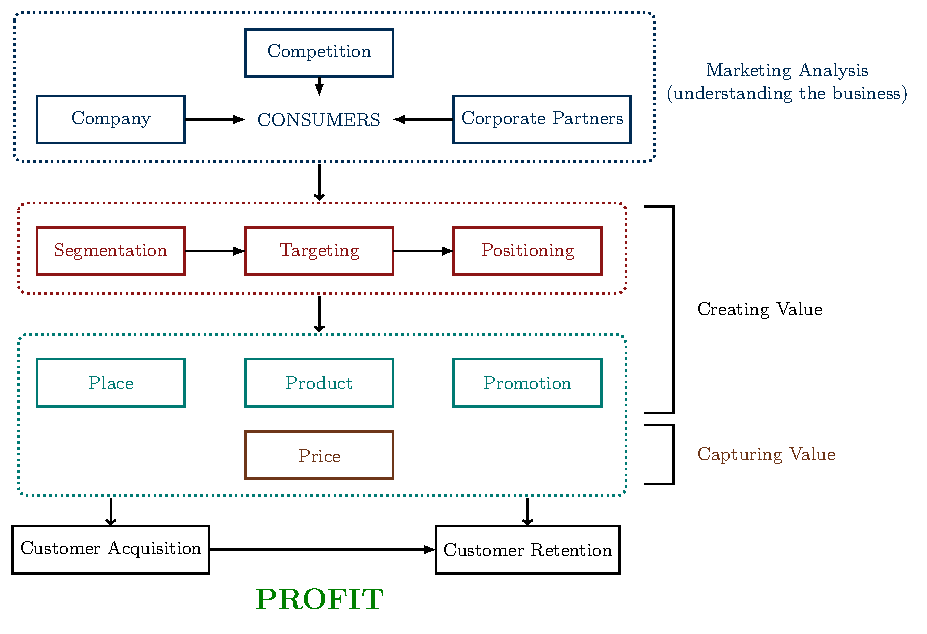
\includegraphics[height=7cm, trim=0.0cm 0.0cm 0.0cm 0.0cm width=7cm]{Big_Picture.pdf}
  \caption{Figure {\color{franklinblue} 26}: The Big Picture}
\end{figure}

\end{frame}

\begin{frame}[t]{Defining Segmentation}
Segmentation, targeting, and positioning, often shortened by marketing analytics professionals to ``STP'', is a core principle of marketing. \empr{Segmentation} means dividing the total market of customers into smaller groups that are alike or \empr{homogeneous}. \\
\vspace{1.5ex}
There are three classifications of marketing segmentation data: demographic, psychographic and behavioral.\\
\vspace{1.5ex}
\begin{enumerate}
\item Demographic Segmentation
\small
\begin{itemize}
 \item Demographic data include customer characteristics like gender, age, income, ethnicity, residence, political affiliation, education level, and customer languages spoken.
 \item The textbook lists 10 external sources of demographic data (e.g., U.S. Census Bureau, Canada Open Data, European Open Data \ldots).
\end{itemize}
\end{enumerate}
\end{frame}

\begin{frame}[t]{Psychographic Segmentation}
\begin{enumerate}
 \setcounter{enumi}{1}
 \item Psychographic Segmentation
 \begin{itemize}
  \item Psychographic data are the psychological characteristics, values, life-stages, and lifestyles of customers.
  \item While more difficult to find, depending on the marketing objective, psychographics are more powerful than demographics because they frequently improve identifying people in their core beliefs. 
  \item \href{https://claritas.com/prizm-premier/}{Claritas} and \href{https://www.esri.com/en-us/home}{Ersi} are vendors of zip code level psychographic data.
  \item \href{https://www.equifax.com/business/product/economic-cohorts/}{Equifax} and \href{https://www.experian.com/marketing-services/mosaic}{Experian} are vendors of household/person level psychographic data.\
  \item  A University of North Carolina \href{https://guides.lib.unc.edu/market-research-tutorial/psychographics}{page} lists several other sources of psychographic data. 
\end{itemize}
\end{enumerate}
\end{frame}

\begin{frame}[t]{Demographic and Psychographic Segmentation View}
Consumers organized on the basis of lifestyle and values. \\
\vspace{1.5ex}
\begin{figure}[htbp]
  \captionsetup{justification=centering}
  \includegraphics[height=5.6cm, trim=0.0cm 0.0cm 0.0cm 0.0cm width=5.6cm]{Images/Psychographic.png}
  \caption{Figure {\color{franklinblue} 27}: Demographic and Psychographic Segmentation Views}
\end{figure}
\end{frame}

\begin{frame}[t]{Behavioral Segmentation}
\begin{enumerate}
 \setcounter{enumi}{2}
 \item Behavioral Segmentation
  \begin{itemize}
    \item Behavioral data is data generated by, or in response to, a customer's engagement with a business. 
    \begin{itemize}
      \item This can include things like page views, email sign-ups, or other important user actions. 
      \item Common sources of behavioral data include websites, mobile apps, CRM systems, marketing automation systems, call centers, help desks, and billing systems.
    \end{itemize}
    \item Similar to demographic data, first-party data is often the best source of behavioral data.
    \item The text book lists 5 external sources of behavioral data (e.g., Nielsen, IRI, \ldots)
  \end{itemize}
\end{enumerate}
\end{frame}

\begin{frame}[t]{Behavioral Segmentation Option Examples}
\begin{figure}[htbp]
  \captionsetup{justification=centering}
  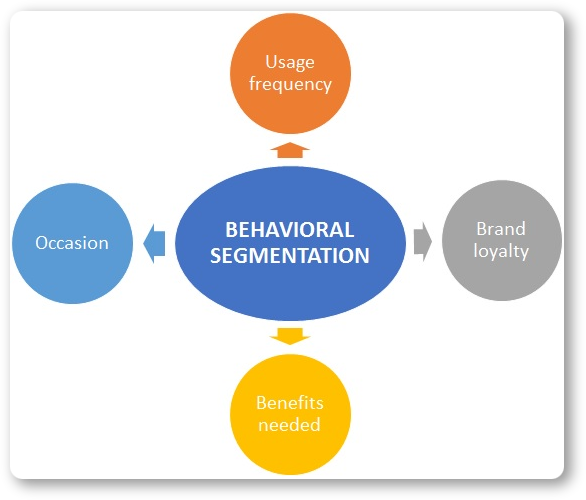
\includegraphics[height=5.6cm, trim=0.0cm 0.0cm 0.0cm 0.0cm width=5.6cm]{Images/Behavioral_Segmentation.png}
  \caption{Figure {\color{franklinblue} 28}: Behavioral Segmentation Options}
\end{figure}
\end{frame}

\begin{frame}[t]{There are Several Other Segmentation Methods}
\small
\begin{table}[htbp]
  \centering
  \captionsetup{justification=centering}
    \begin{tabular}{|cl|}
    \toprule
   % \rowcolor[rgb]{ .851,  .882,  .949} \textbf{Sample} & \textbf{Sample Mean} & \textbf{Sample} & \textbf{Sample Mean} & \textbf{Sample} & \textbf{Sample Mean}  \\
   \textbf{{\color{franklinblue} Segmentation }} & \textbf{{\color{franklinblue} Sample Segments}} \\
   \midrule
  \multirow{4}*{Geographic} & Continent: North America, Asia, Europe\\
   & South America, Africa \\
   & Within the United States: Pacific, Mountain,  \\
   & Central, South, Mid-Atlantic, Northeast. \\
  \midrule
  Demographic & Age, gender, income \\
  \midrule
  Psychographic & Lifestyle, life-stage, self-concept, self-values \\
  \midrule
  Benefits & Convenience, economy, prestige \\ 
  \midrule
  Behavioral & Occasion, loyalty, usage, benefits \\
  \bottomrule
     \end{tabular}%
  \caption{Segmentation Methods}
  \label{tab:seg1}%
\end{table}%
\end{frame}

\begin{frame}[t]{Targeting }
\empr{Targeting} means appealing to particular segments of customers.  There are three main strategies for targeting: differentiated, concentrated, and undifferentiated targeting. \\
\vspace{1.5ex}
\small
\begin{itemize}
  \item \empr{Differentiated targeting} is when a firm targets each of the potential segments it discovers, each with a different marketing mix. For example, \href{https://www.petsmart.com/}{Petsmart's} organic dog food category manager is looking to target a specific type of person - a health conscious, animal loving and eco-friendly individual;  thus this segment will receive different (say) emails than those of other segments. 
 \item \empr{Concentrated targeting} is when a firm focuses on a single market segment. For example, \href{https://www.gmc.com/electric/hummer-ev}{GMC Hummer} focus is on those who favor rugged country and off-roading. 
 \item \empr{Undifferentiated targeting}, which is not recommended, means firms ignore the data on segmentation and offer the same marketing effort to everyone in the population. 
\end{itemize}
\end{frame}

\begin{frame}[t]{Positioning}
\empr{Positioning} is a marketing strategy that establishes the way a customer perceives a product or firm relative to the rest of the marketplace. \\
\vspace{1.5ex} 
This is accomplished by changing the marketing mix -- what the product is like, what its price is, where customers purchase it, and how it is promoted. \\
\vspace{1.5ex}
 Positioning is distinct from targeting. Targeting is identifying which segment(s) to pursue, and positioning is the way a business tries to affect the way people in the targeted segments perceive it by changing its marketing mix.
\end{frame}

\section{Segmentation, Targeting and Positioning Implementation}

\begin{frame}[t]{The 6 Steps for STP Implementation}
There are six steps to implementing STP using data. \\
\vspace{1.5ex}
The steps can be accomplished using a number of data analytics techniques.\\
 \vspace{0.0ex}
\begin{figure}[htbp]
  \captionsetup{justification=centering}
  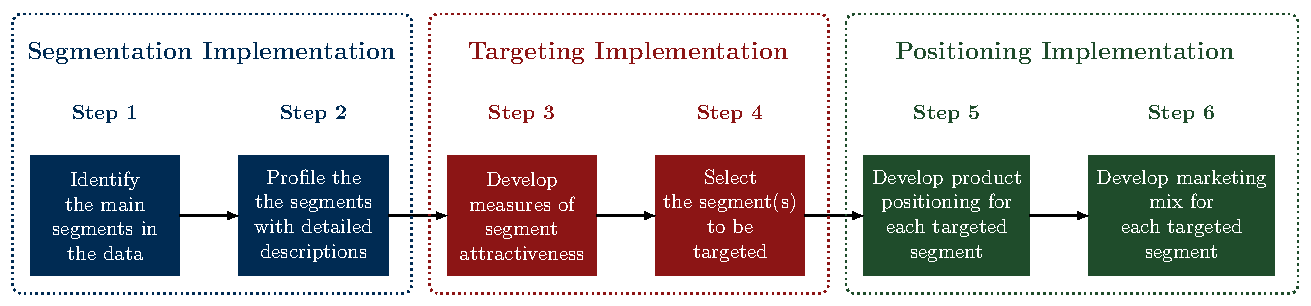
\includegraphics[height=2.8cm, trim=1.0cm 0.0cm 0.0cm 0.0cm width=2.8cm]{STP_Process.pdf}
  \caption{Figure {\color{franklinblue} 29}: STP Implementation Steps}
\end{figure}
\end{frame}

\begin{frame}[t]{Identifying Segments by Statistical Learning}
\textbf{\color{franklinblue} Step 1} \\
\vspace{1.5ex}
\empr{Statistical learning} refers to a large set of supervised and unsupervised tools for understanding data. 
\begin{enumerate}
\item \empr{Supervised statistical learning} involves building a statistical model for predicting, or estimating, an output based on one or more inputs. 
\begin{itemize}
\item Problems of this nature occur in fields as diverse as astrophysics, business, economics, medicine, and psychology. 
\item Examples of methods include:
\begin{enumerate}
  \item Linear regression
  \item Logistic regression
  \item Naive Bayes classifiers 
  \item Kernel regression
\end{enumerate}
\end{itemize}
\end{enumerate}
\end{frame}

\begin{frame}[t]{Supervised Learning Methods Continued}
\begin{enumerate}
\item []
\begin{itemize}
\item []
\begin{enumerate}
\item [1.5] Local polynomial regression
\item [1.6] Regression splines
\item [1.7]  Smoothing splines 
\item [1.8] Generalized additive models\footnote{Kernel regression, local polynomial regression, regression splines, smoothing splines and generalized additive models are \empr{semiparametric regression} approaches.  For additional information about semiparametric regression, see \cite{rupert2009}.} 
\item [1.8] Penalized regression\footnote{Examples include ridge regression, lasso regression, and elastic net regression.  For a discussion of these methods see \cite{zou2005}.}
\item [1.10] Decision tress
\item [1.11] Random forests and other ensemble model approaches
\end{enumerate}
\end{itemize}
\end{enumerate}
\end{frame}

\begin{frame}[t]{SVM and Neural Networks}
\begin{enumerate}
\item []
\begin{itemize}
\item []
\begin{enumerate}
\item [1.12] Support vector machines (SVM)
\item [1.13] Neural networks, also known as artificial neural networks or simulated neural networks\footnote{The four basic neural network specifications are multilayer perceptrons, convolutional neural networks, radial basis functional neural networks, and recurrent neural networks.  A neural network with multiple hidden layers and multiple nodes in each hidden layer is known as a \empr{deep learning system} or a \empr{deep neural network}.  The word ``deep'' in Deep Learning refers to the number of hidden layers -- depth of the neural network.  For an introduction to the most basic network structures, see \cite{james2021}. For a review of deep learning concepts,  architectures, challenges, applications, and future directions see \cite{alzubaidi2021beamerissue}.}. 
\end{enumerate}
\end{itemize}
\end{enumerate}
\end{frame}

\begin{frame}[t]{Unsupervised Learning}
\begin{enumerate}
  \setcounter{enumi}{1}
\item With \empr{unsupervised statistical learning}, there are inputs but no supervising output; nevertheless we can learn relationships and structure  from such data.
\begin{itemize}
\item Unsupervised learning is a set of statistical tools intended for the setting in which we have only a set of \empr{features} $X_1,X_2,\ldots, X_p$ measured on $n$ observations.\footnote{A feature may also be referred to as an attribute, characteristic or variable.} 
\item We are not interested in prediction, because we do not have an associated \empr{response variable} $Y$. Rather, the goal is to discover interesting things about the measurements on $X_1, X_2,\ldots,X_p$.  Two unsupervised learning types are:  
\begin{enumerate}
\item \empr{Principal components analysis} (PCA) is a tool used for data visualization or data pre-processing before supervised techniques are applied.
\item \empr{Clustering} is  a broad class of methods for discovering unknown subgroups in data, such as in STP.
\end{enumerate}
\end{itemize}
\end{enumerate}
\end{frame}

\begin{frame}[t]{Fundamentals of Clustering}
When we cluster the observations of a data set, we seek to partition them into distinct groups so that the observations within each group are quite similar to each other, while observations in different groups are quite different from each other. \\
\vspace{1.5ex}
To make this concrete, we must define what it means for two or more observations to be similar or different. The method chosen to conduct clustering yields specificity on similarity. \\
\vspace{1.5ex}
There are many cluster analysis algorithms. The two best-known clustering approaches are \empr{$K$-means clustering}, where we choose the number of clusters, and \empr{hierarchical clustering}. \\
\vspace{1.5ex}
In hierarchical clustering, we do not know in advance how many clusters we want. Thus a tree-like visual representation of the combining of observations into clusters is produced. This visualization is called a \empr{dendrogram}. 
\end{frame}

\begin{frame}[t]{A Dendrogram}
\begin{figure}[htbp]
  \captionsetup{justification=centering}
  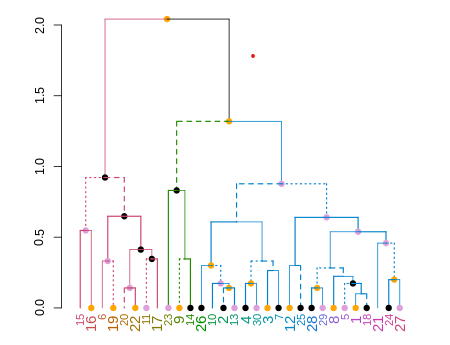
\includegraphics[height=5.8cm, trim=0.0cm 0.0cm 0.0cm 0.0cm width=5.8cm]{Images/Dendrogram_Example.png}
  \caption{Figure {\color{franklinblue} 30}: A Dendrogram}
\end{figure}
\vspace{-2.0ex}
The distance between clusters is on the ordinate and the observations on the abscissa.
\end{frame}

\begin{frame}[t]{$K$-Means Clustering}
$K$-means clustering is a simple and elegant approach for partitioning a
data set into $K$ distinct, non-overlapping clusters.\footnote{The source for much of the information that follows on clustering was sourced from \cite{hastie2009}.  Another excellent introduction to clustering is \cite{everitt2011}.} To perform $K$-means clustering, we must first specify the desired number of clusters $K$; then the $K$-means algorithm will assign each observation to exactly one of the $K$ clusters. \\
\vspace{1.5ex}
Let $C_1, C_2 \ldots, C_K$ denote sets containing the indices of the observations in each cluster. These sets satisfy 2 properties: \\
\vspace{0.0ex}
\small
\begin{enumerate}
\item $C_1 \cup C_2 \ldots \cup C_K = {1,2,\ldots,n}$.  That is, each observation
belongs to at least one of the K clusters.
\item $C_i \cap C_j = \emptyset, \; \forall i \neq j$. Thus the clusters are non-overlapping (i.e., no observation belongs to more than one cluster).
\end{enumerate}
\end{frame}

\begin{frame}[t]{Determining ``Good'' Clustering}
 The idea behind $K$-means clustering is that a ``good ''clustering is one for which the \empr{within-cluster variation} is as small as possible.\footnote{As a secondary objective, we would like to have large \empr{between-cluster variation}.} \\ 
\vspace{1.5ex}
The within-cluster variation for cluster $C_k$ is a measure $W(C_k)$ of the amount by which the observations within a cluster differ from each other.  \\
\vspace{1.5ex}
Therefore we want to solve the problem, \\
\vspace{0.0ex}
\begin{equation}\label{eq1}
\underset{C_1, C_2 \ldots, C_K}{\text{minimize}} \bigg\{ \sum_{k=1}^{K} W(C_k) \bigg\}.
\end{equation}
Let $x_{ij}$ be the $j$th feature of observation (e.g., person) $i$.  The features are used to determine the clusters. 
\end{frame}

\begin{frame}[t]{Specifying the Clustering Objective}
To make Equation (\ref{eq1}) operational, we need to choose a specification for $W$.  While there are many possible specifications, the most common choice uses \empr{squared Euclidean distance}.  \\
\vspace{-0.5ex}
\begin{equation}\label{eq2}
W(C_k) = \frac{1}{\abs{C_k}} \sum_{i,i' \in C_k} \sum_{j=1}^{p}(x_{ij} - x_{i'j})^2,
\end{equation}
where $\abs{C_k}$ is the number of observations in the $k^{th}$ cluster.  Combining Equations (\ref{eq1}) and (\ref{eq2}), we have, \\
\vspace{-0.5ex}
\begin{equation}\label{eq3}
\underset{C_1, C_2 \ldots, C_K}{\text{minimize}} \bigg\{ \sum_{k=1}^{K} \frac{1}{\abs{C_k}} \sum_{i,i' \in C_k} \sum_{j=1}^{p}(x_{ij} - x_{i'j})^2 \bigg\}.
\end{equation}
Finding a solution for Equation (\ref{eq3}) is a very difficult problem to solve
precisely since there are almost $K^n$ ways to partition $n$ observations into $K$
clusters.%  This is a huge number unless $K$ and $n$ are tiny!
\end{frame}

\begin{frame}[t]{Solving the Clustering Objective}
The following algorithm is guaranteed to decrease the value of the objective
at each step. \\
\vspace{1.5ex}
\begin{enumerate}
\item Randomly assign a number, from 1 to $K$, to each of the $n$ observations. These serve as initial cluster assignments for the observations.
\item Iterate until the cluster assignments stop changing:
\begin{enumerate} 
  \item For each of the $K$ clusters, compute the cluster \empr{centroid}. The $k$th cluster centroid is the vector of the $p$ feature means for the observations in the $k$th cluster.\footnote{More generally, a centroid is the center of a geometric object's internal mass, assuming uniform density.}
  \item  Assign each observation to the cluster whose centroid is closest (where closest is defined using Euclidean distance).
\end{enumerate}
\end{enumerate} 
\end{frame}

\begin{frame}[t]{Choosing the Number of $K$-Means Clusters}
Determining the number of clusters is a hard and important problem.  There is no efficient and universal method for identifying the initial partitions and the number of clusters $K$.\footnote{For a survey of a few statistical methods used to determine the number of clusters, see \cite{chiang2010}.}\\
\vspace{1.5ex}
Managerial Approach to Choosing the Number of Clusters \\
\vspace{0.0ex}
\small
\begin{enumerate}
  \item  Determine the maximum number clusters that could be targeted.  This is a function of company resources. 
  \item  After conducting a $K$-means cluster analysis, consider the proportion or number of people per cluster.  If the proportion or number is too small to target, than reduce the number of clusters.  
  \item Ensure there is sufficient differentiation between segments.  Thus measures of between segment variation are important to review.   
\end{enumerate}
\end{frame}

\begin{frame}[t]{Sidebar About PCA and Clustering}
PCA plots are frequently used to find potential clusters by simplifying the complexity in high-dimensional data while retaining trends and patterns.  \\
\vspace{1.5ex} 
This reduction in  the dimensionality of a data set is accomplished by linearly transforming the data into a new coordinate system where (most of) the \underline{variation} in the data can be described with fewer dimensions than the initial data.  That is, PCA reduces data dimensionality by geometrically projecting it onto lower dimensions called \textit{principal components} (PCs). 
\small
\vspace{-1.0ex}
\begin{itemize}
\item All PCs, linear combinations of the original variables, beyond the first are required to be \underline{uncorrelated} with all previous PCs.
\item  PCs are very useful for clustering in the presence of the \empr{curse of dimensionality}.\footnote{For additional information on using PCA to detect the number of clusters see \cite{lever2017}.} 
\end{itemize}
\end{frame}

\begin{frame}[t]{The Curse of Dimensionality}
High dimensional data refers to data with a large number of features, variables or dimensions often represented by the columns in a data set, where each row is an instance or observation. Frequently, the number of variables (columns) can exceed the number of observations (rows).\\
\vspace{1.5ex}
The term ``curse of dimensionality'' refers to the difficulty of dynamic optimization with many variables.\footnote{The curse of dimensionality may be restated as, ``As the number of features or dimensions grows, the amount of data we need to generalize accurately grows exponentially.'' The term ``curse of dimensionality'' was coined in \cite{bellman1957}.} Broadly, the following issues are faced when working with high dimensional data.
\begin{enumerate}
  \item Working with large dimensional data is computational challenging. The processing and storing of high dimensional data require substantially more computational resources. 
\end{enumerate}
\end{frame}

\begin{frame}[t]{Accuracy Degradation \& the Curse of Dimensionality}
\begin{enumerate}
  \setcounter{enumi}{1}
  \item Working with large dimensional data is computational challenging. The processing and storing of high dimensional data require substantially more computational resources. 
  \item Large dimensional data is very hard to visualize and interpret.\footnote{PCA assists on overcoming this issue.}
  \item Generally as number of features increases redundancy also increases -- more noise is added to data than signal. This results in degradation of performance of all analytic methods. 
\end{enumerate}
\end{frame}

\begin{frame}[t]{A Curse of Dimensionality Example}
Suppose during the last 2 years a B-to-B construction equipment and material supplier serviced 1,024 customers. \\
\vspace{1.5ex}
The company's marketing department decides to partition customers based on purchase recency in days, say by creating a variable defined as 1 divided by the number of days since last purchase, $R$, and 2 year total monetary value, $M$, using quartiles.  Thus 25\% of customers will have a recency between $Q_{0,R}$ (i.e., the minimum of $R$) and $Q_{1,R}$, 25\% will have a recency between $Q_{1,R}$ and $Q_{2,R}$, \ldots, and 25\%  will have a a monetary value between $Q_{3,M}$ and $Q_{4,M}$.  There are $4^2 = 16$ $R$ and $M$ combinations.  \\
\vspace{1.5ex}
If the 1,024 customers are randomly distributed among each $R$ and $M$ combination, then on average there are 64 customers within each possible combination, which is a good enough sample to draw conclusions. If for example customer $i$, $R_i \in [Q_{0,R},Q_{1,R}]$ and $M_i \in [Q_{0,M},Q_{1,M}]$, we may infer the customer has attrited. \\
\end{frame}

\begin{frame}[t]{The Curse of Dimensionality Example Continued}
Now suppose the marketing department decides to expand the analysis to make it a Recency-Frequency-Monetary Value (RFM) analysis supplemented by the number of items purchased by the customer.  If frequency $F$ and number of items $I$ are partitioned into quartiles, then there are $4^4 = 256$ combinations. \\
\vspace{1.5ex} 
Assuming again customers are randomly distributed across the 4 combinations, the average number of customers per combination is 4. \\
\vspace{1.5ex}
If the analysis is expanded from 4 variables to 8 variables and quartiles are still used to define partitions, then there are $4^8 = 65,536$ combinations with an average number of customers per combination equal to 0.0156.  This means that almost all possible combinations are never observed, and the company has realized the curse of dimensionality.
\end{frame}

\begin{frame}[t]{Profiling Segments}
\textbf{\color{franklinblue} Step 2} \\
\vspace{1.5ex}
Once segments have been determined, we will want identify which people are in the segments by \empr{profiling} them.   \\
\vspace{1.5ex}
A simple profiling method is calculate average characteristics (e.g., age, income, \ldots)  and proportions (e.g., gender, lifestyle segments, life-stage segments, \ldots)  for all people assigned to a particular segment.  \\
\vspace{1.5ex}
Once this has been done, it is customary to name the segments.  Such as \textit{Fashionista}, \textit{Deal Shopper}, \textit{Premium Buyer}, \dots
\end{frame}

\begin{frame}[t]{Segment Attractiveness and Selecting Segments}
\textbf{\color{cardinalred} Step 3} \\
\vspace{1.5ex}
Next, we would like to know which segments are most attractive according to criteria such as past sales. We can also compare means on marketing outcome variables like customer satisfaction, loyalty, revenue or profits. \\
\vspace{1.5ex}
The process is similar to that of profiling the segments.\\
\vspace{1.5ex}
\textbf{\color{cardinalred} Step 4} \\
\vspace{1.5ex}
The marketing analytics professional work with management to decide which segment(s) to target based on business objectives.
\end{frame}

\begin{frame}[t]{Product Positioning and Marketing Mix}
\textbf{\color{calpolypomonagreen} Step 5} \\
\vspace{1.5ex}
Once we have identified the targeted segments, we will need to determine how to position the company differently across segments.  \\
\vspace{1.5ex}
A simple means profiling analyses on marketing mix variables could be useful to learn about what each segment might value in the company's positioning. \\
\vspace{1.5ex}
\textbf{\color{calpolypomonagreen} Step 6} \\
\vspace{1.5ex}
The final step in the STP is to use the data on product positioning for each targeted segment to develop a marketing mix plan for each target segment using the 4 or 7 P's.
\end{frame}

\section{References}

%https://latex-beamer.com/faq/long-bibliographies-beamer/
%https://github.com/jgm/pandoc/issues/2442
\widowpenalties 1 10000
\small
\bibliography{../../Bibliography/list2}
\bibliographystyle{apalike}

\end{document}